
\chapter{Supplementary material for $HH$ searches}

\section{Additional plots for fake-background estimation}
\label{sec:appendix:fakes}
\begin{figure}
  \centering
  \subfloat[$N_{\text{jets}} = 2$] { 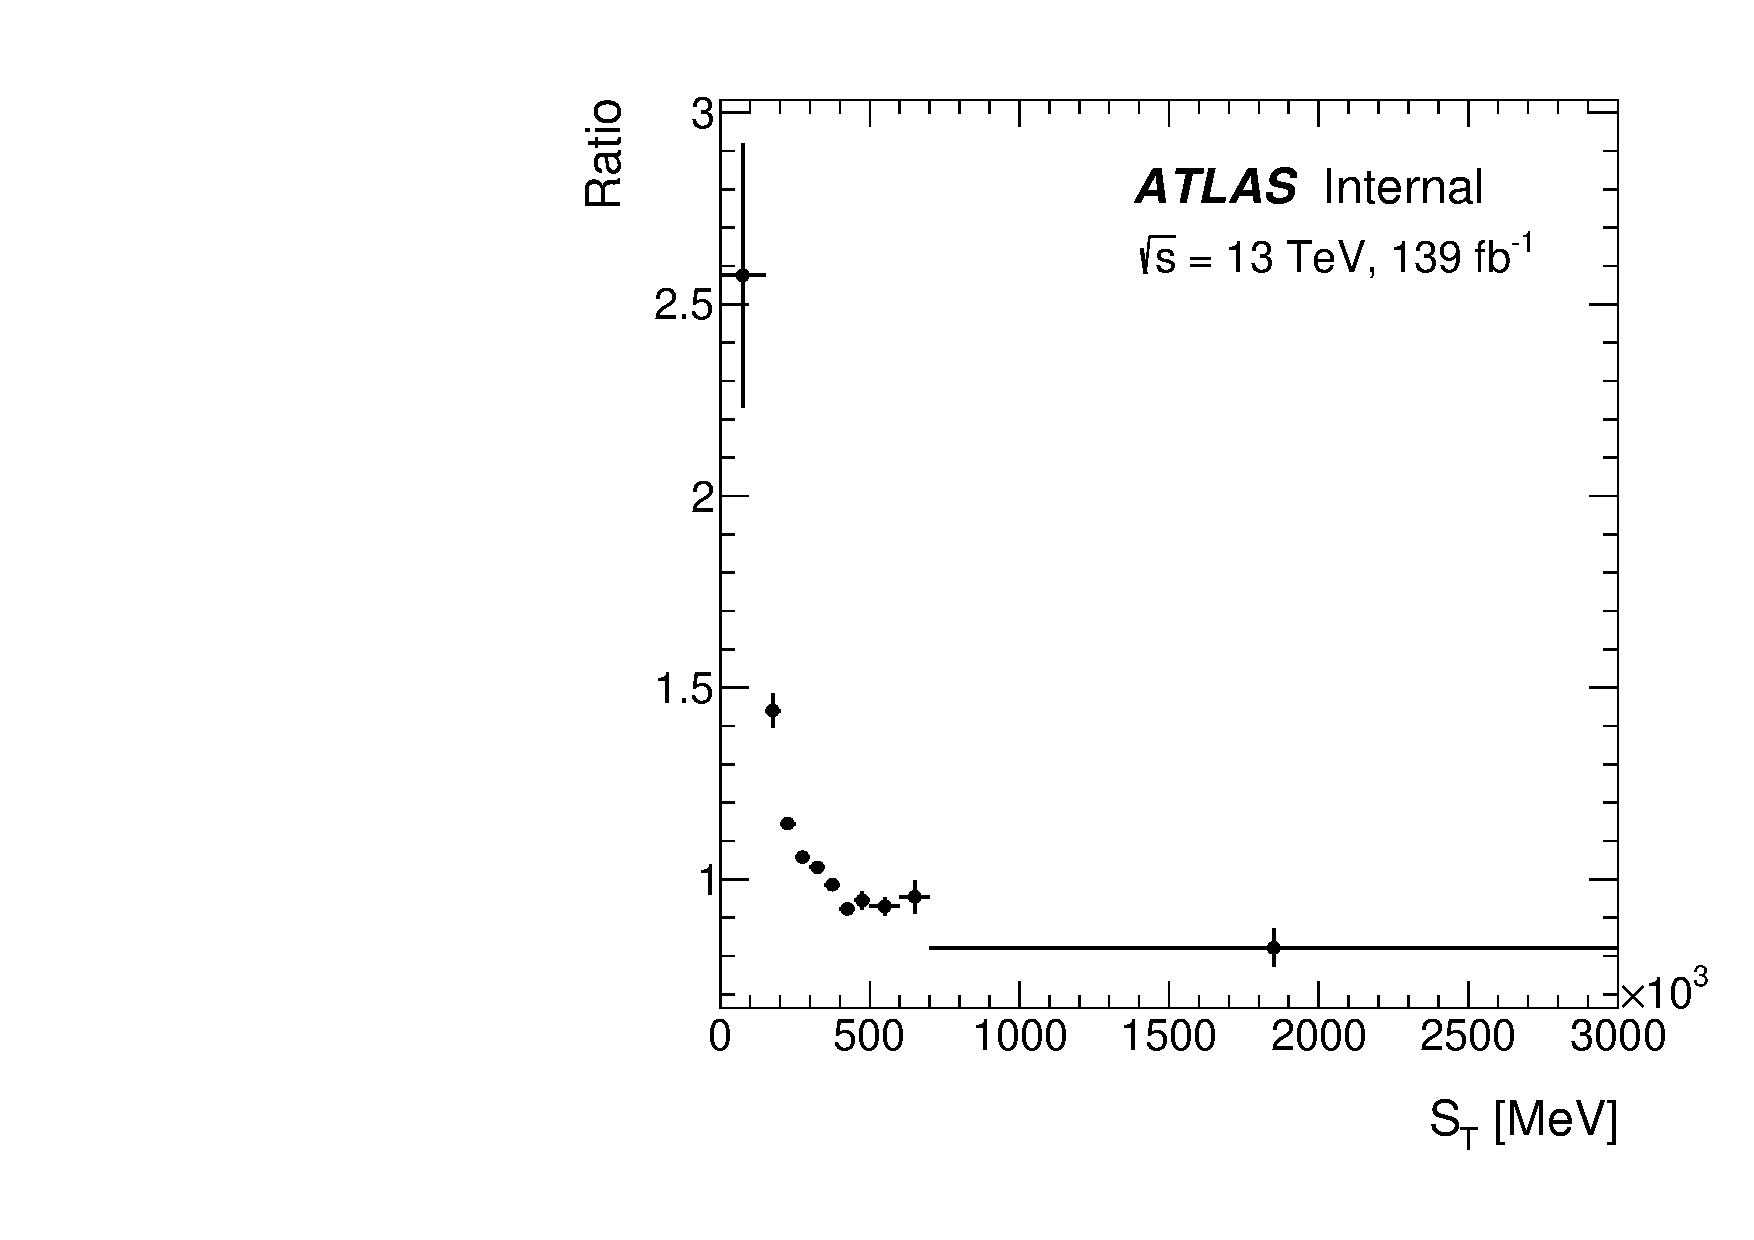
\includegraphics[width=.32\textwidth]{DiHiggs/plots/TtbarReweighting/wt1d_st_fr_os_2.pdf} }
  \subfloat[$N_{\text{jets}} = 3$] { 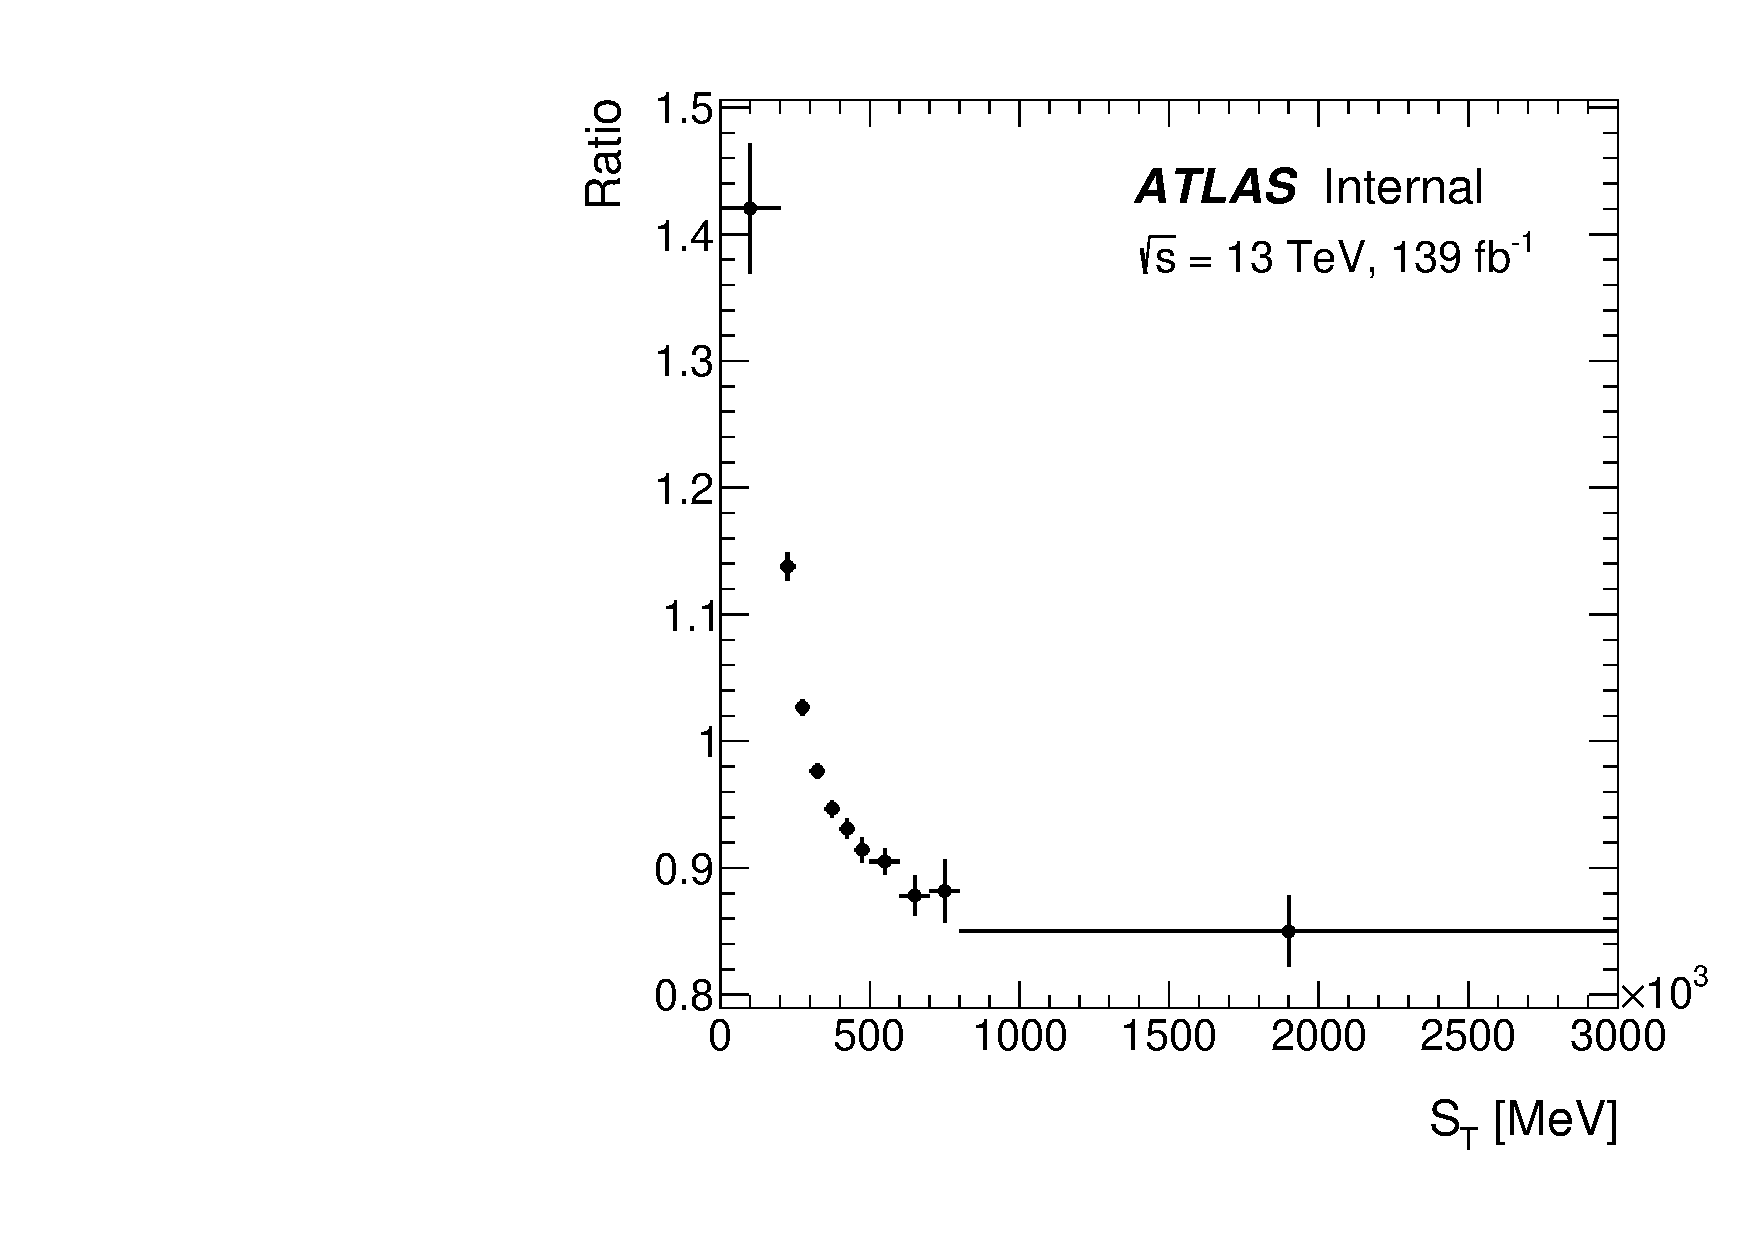
\includegraphics[width=.32\textwidth]{DiHiggs/plots/TtbarReweighting/wt1d_st_fr_os_3.pdf} }
  \subfloat[$N_{\text{jets}} = 4$] { 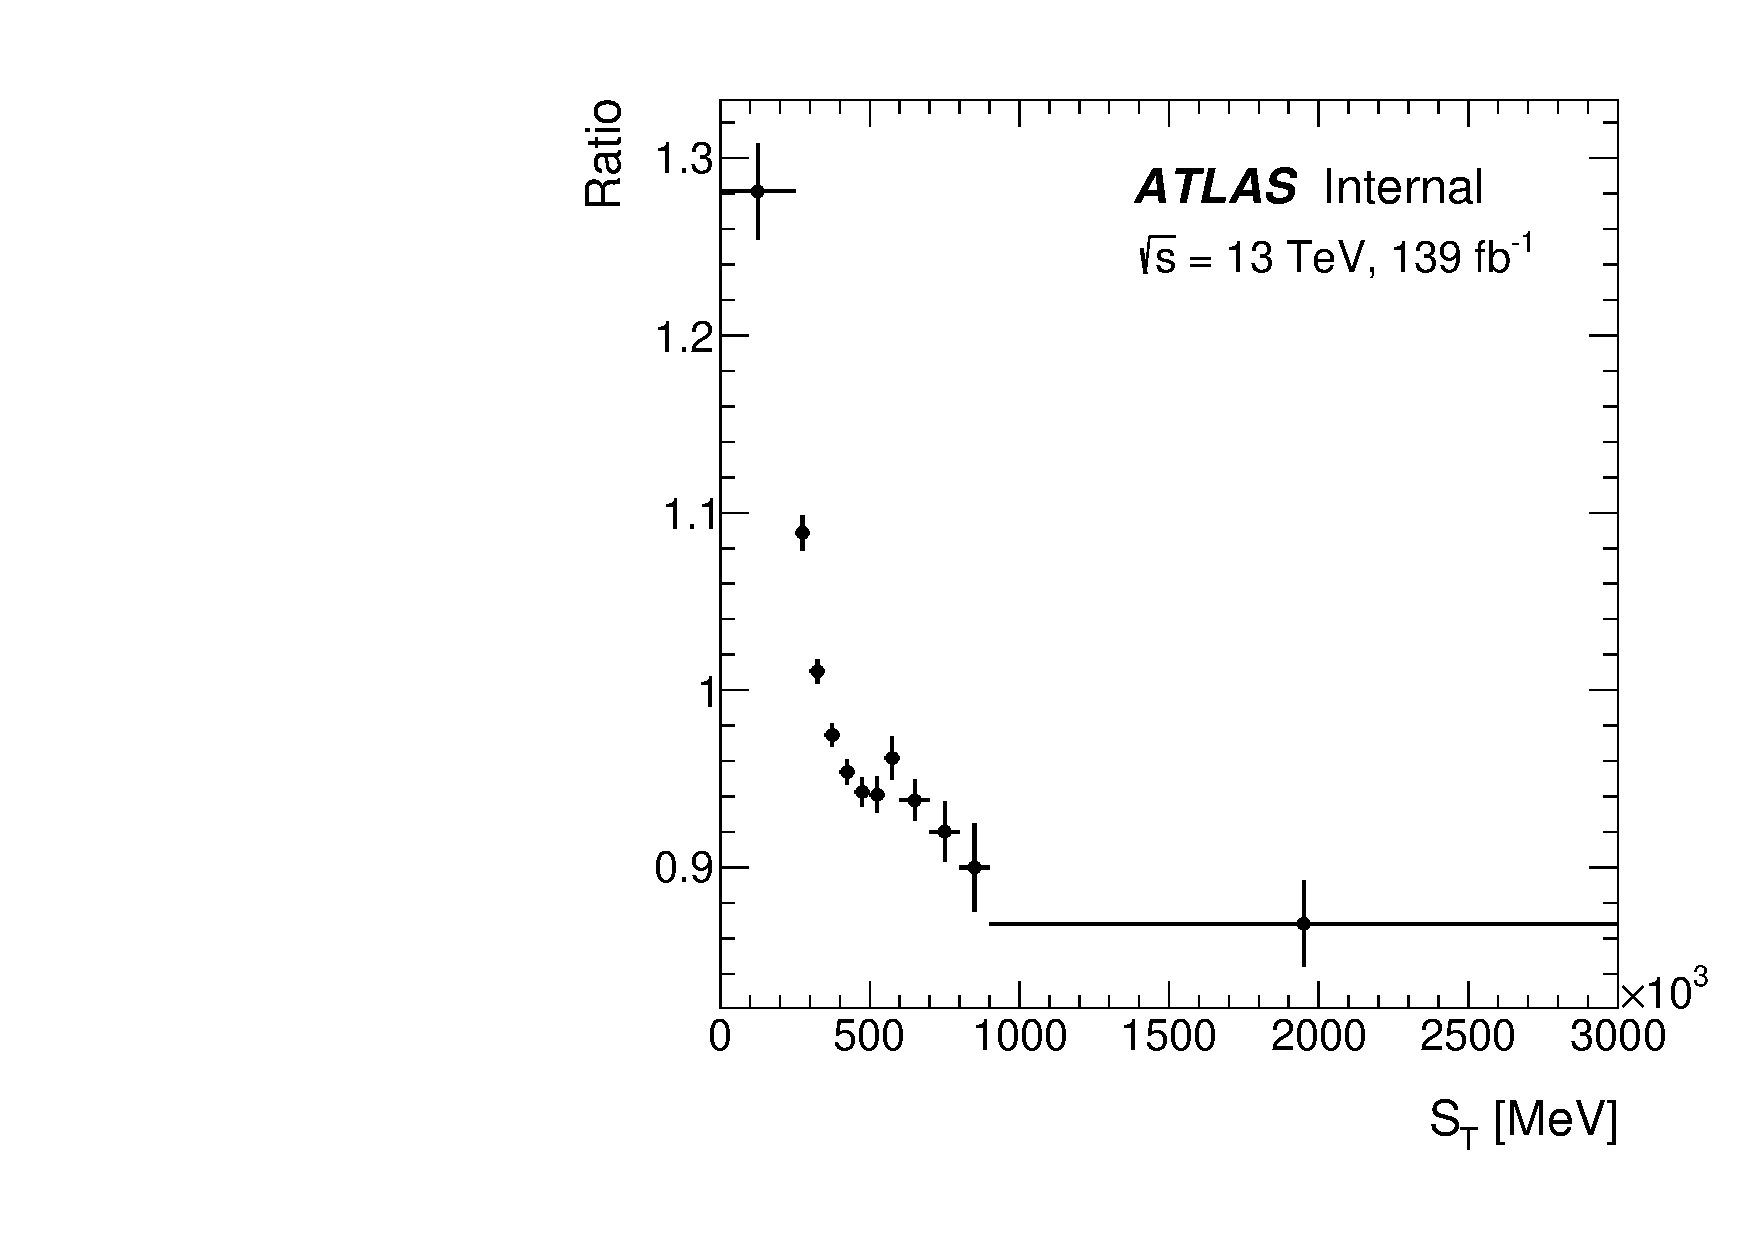
\includegraphics[width=.32\textwidth]{DiHiggs/plots/TtbarReweighting/wt1d_st_fr_os_4.pdf} } \\
  \subfloat[$N_{\text{jets}} = 5$] { 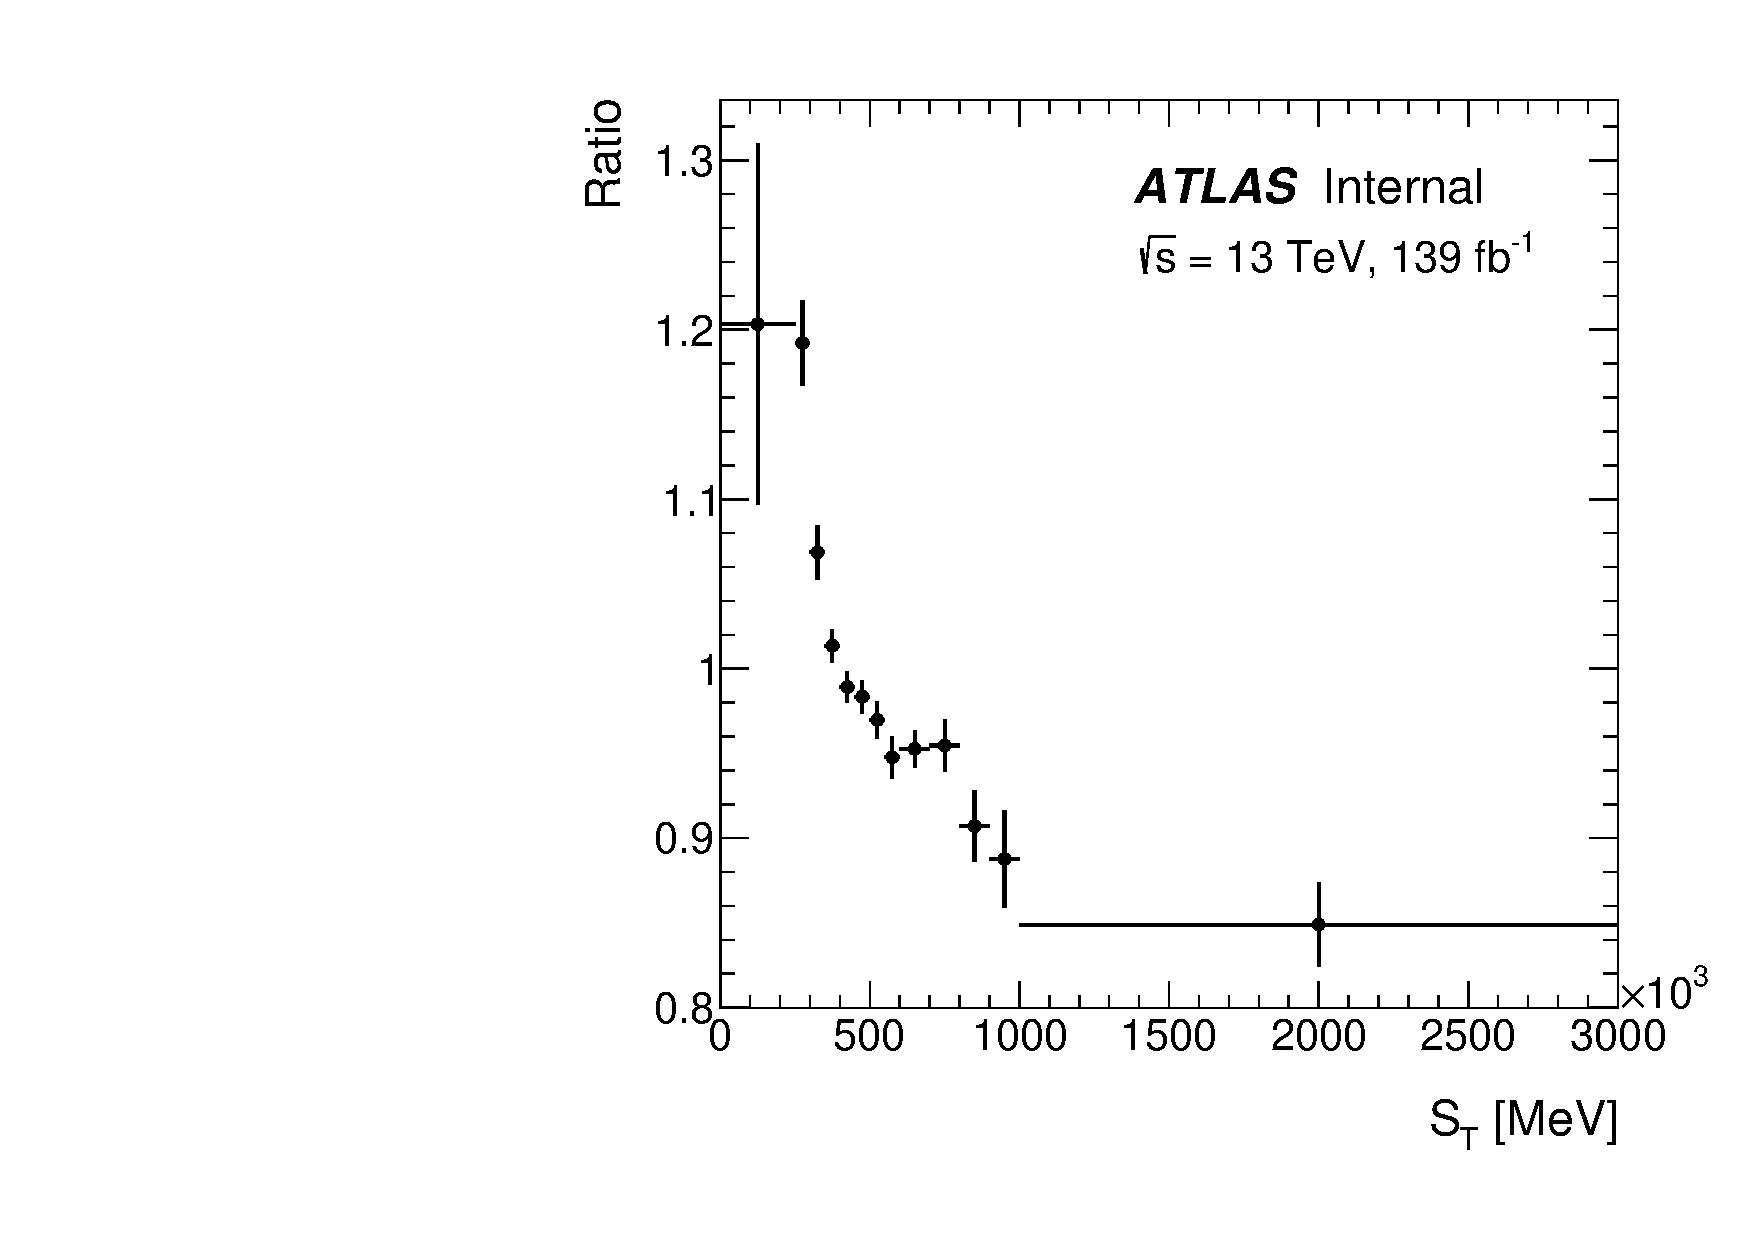
\includegraphics[width=.32\textwidth]{DiHiggs/plots/TtbarReweighting/wt1d_st_fr_os_5.pdf} }
  \subfloat[$N_{\text{jets}} = 6$] { 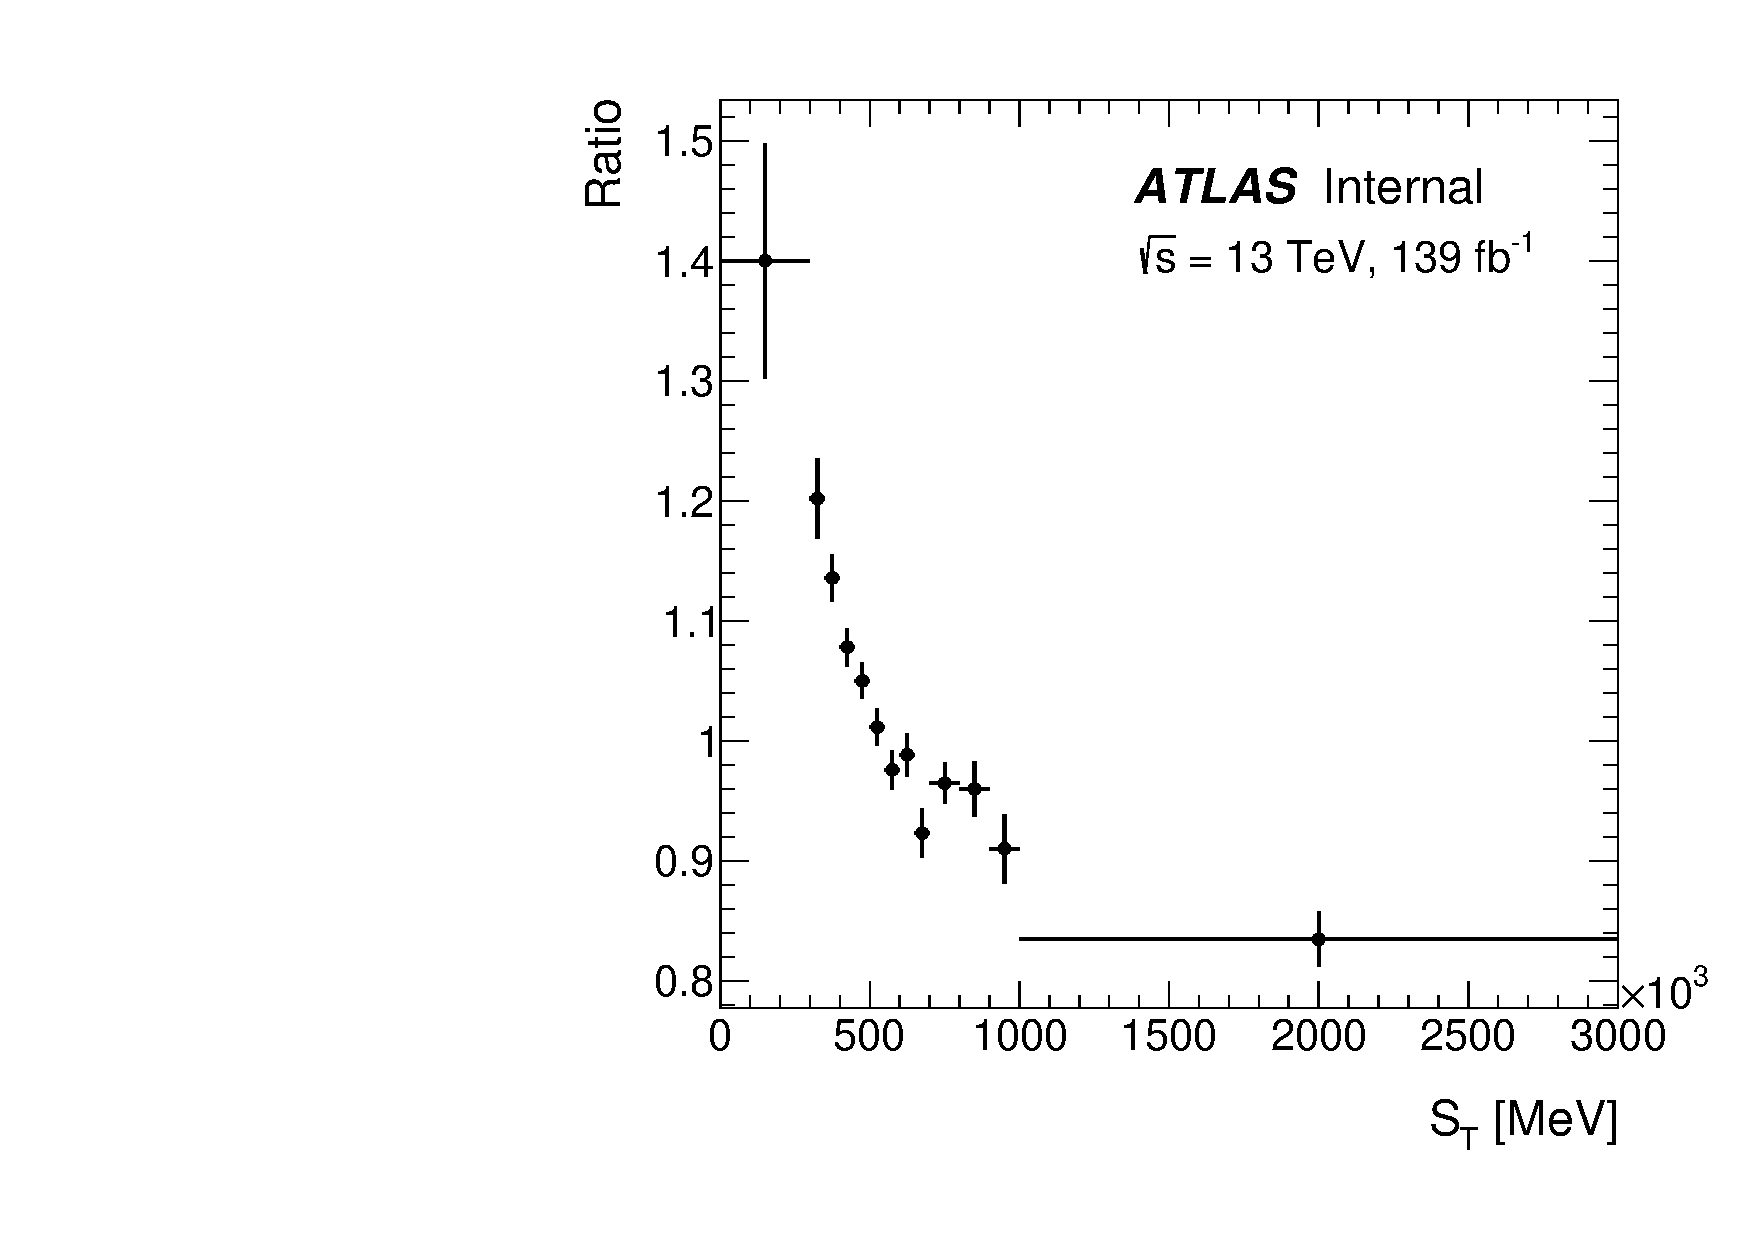
\includegraphics[width=.32\textwidth]{DiHiggs/plots/TtbarReweighting/wt1d_st_fr_os_6.pdf} }
  \subfloat[$N_{\text{jets}} = 7$] { 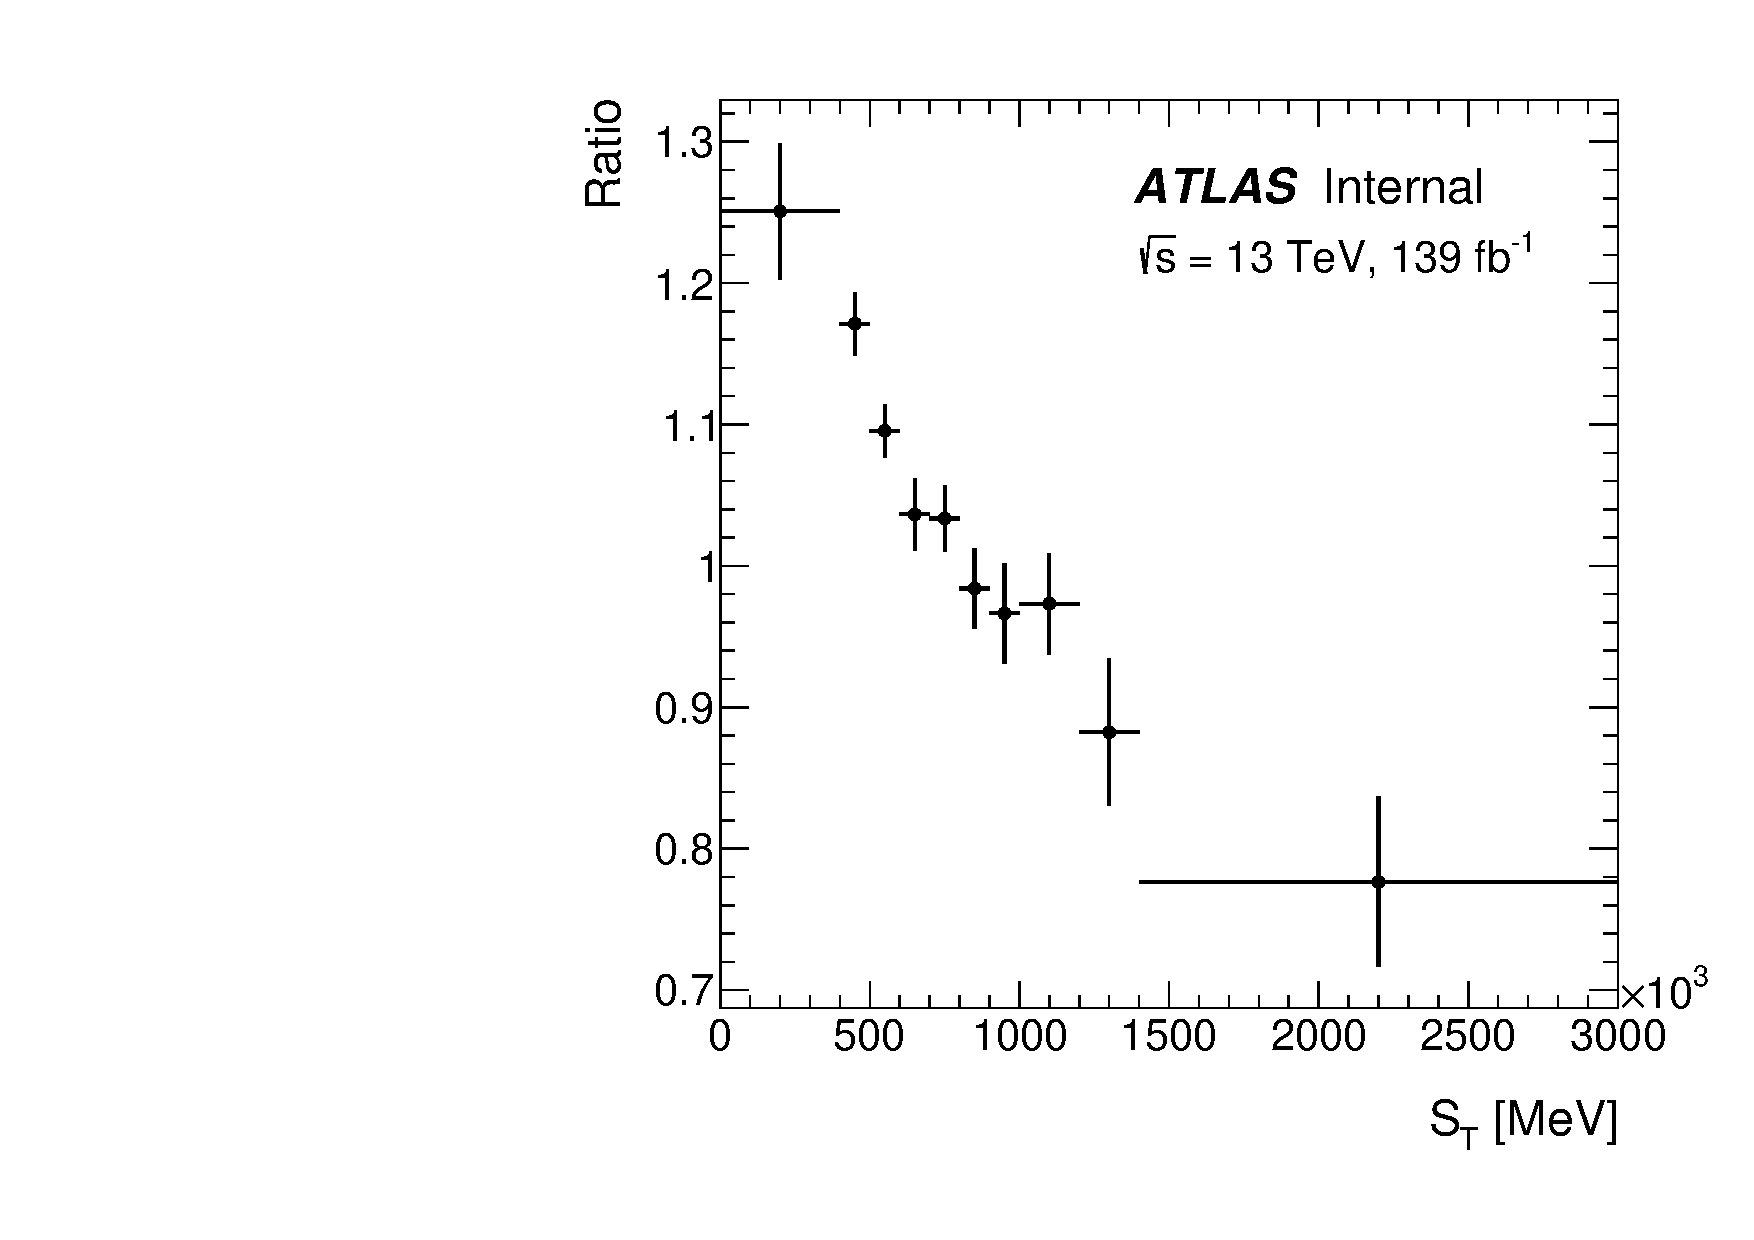
\includegraphics[width=.32\textwidth]{DiHiggs/plots/TtbarReweighting/wt1d_st_fr_os_7.pdf} } \\ 
  \subfloat[$N_{\text{jets}} = 8$] { 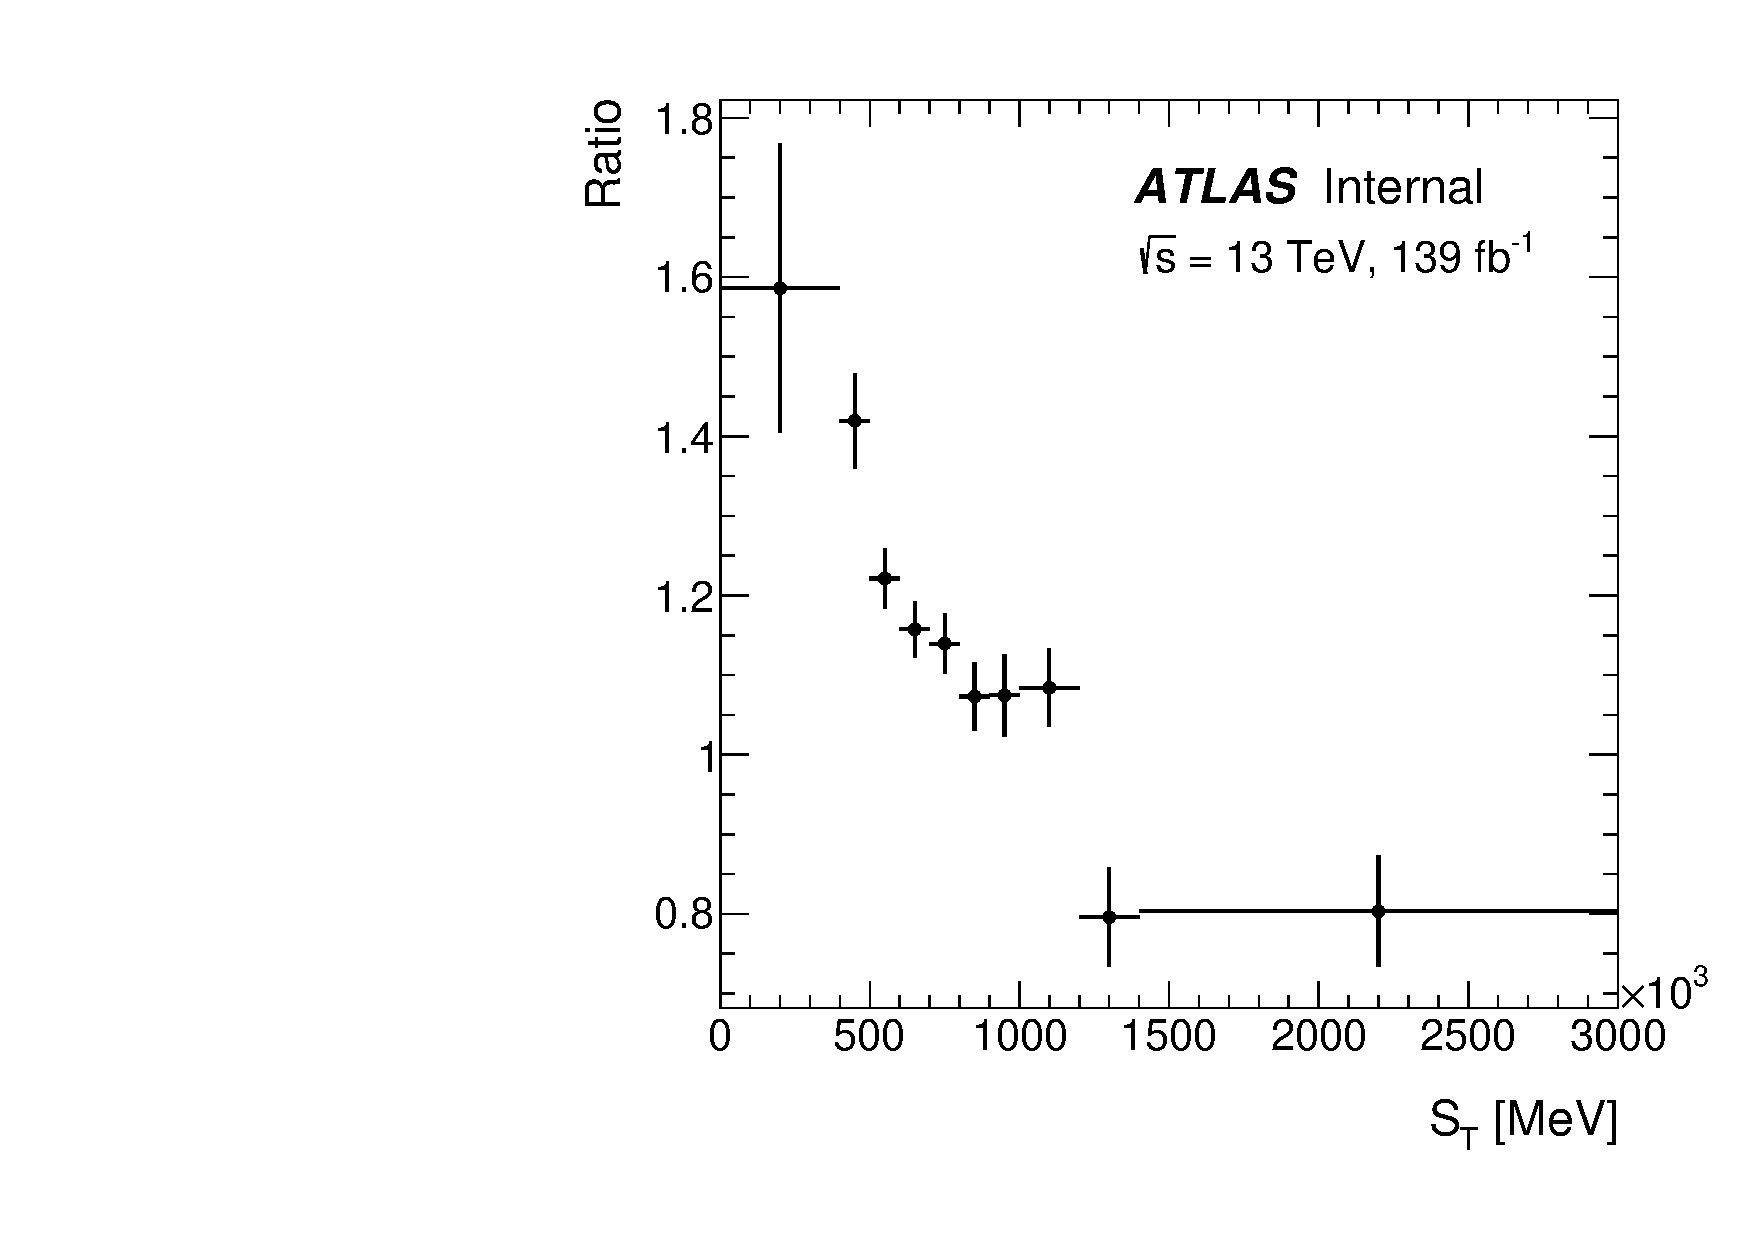
\includegraphics[width=.32\textwidth]{DiHiggs/plots/TtbarReweighting/wt1d_st_fr_os_8.pdf} }
  \subfloat[$N_{\text{jets}} = 9$] { 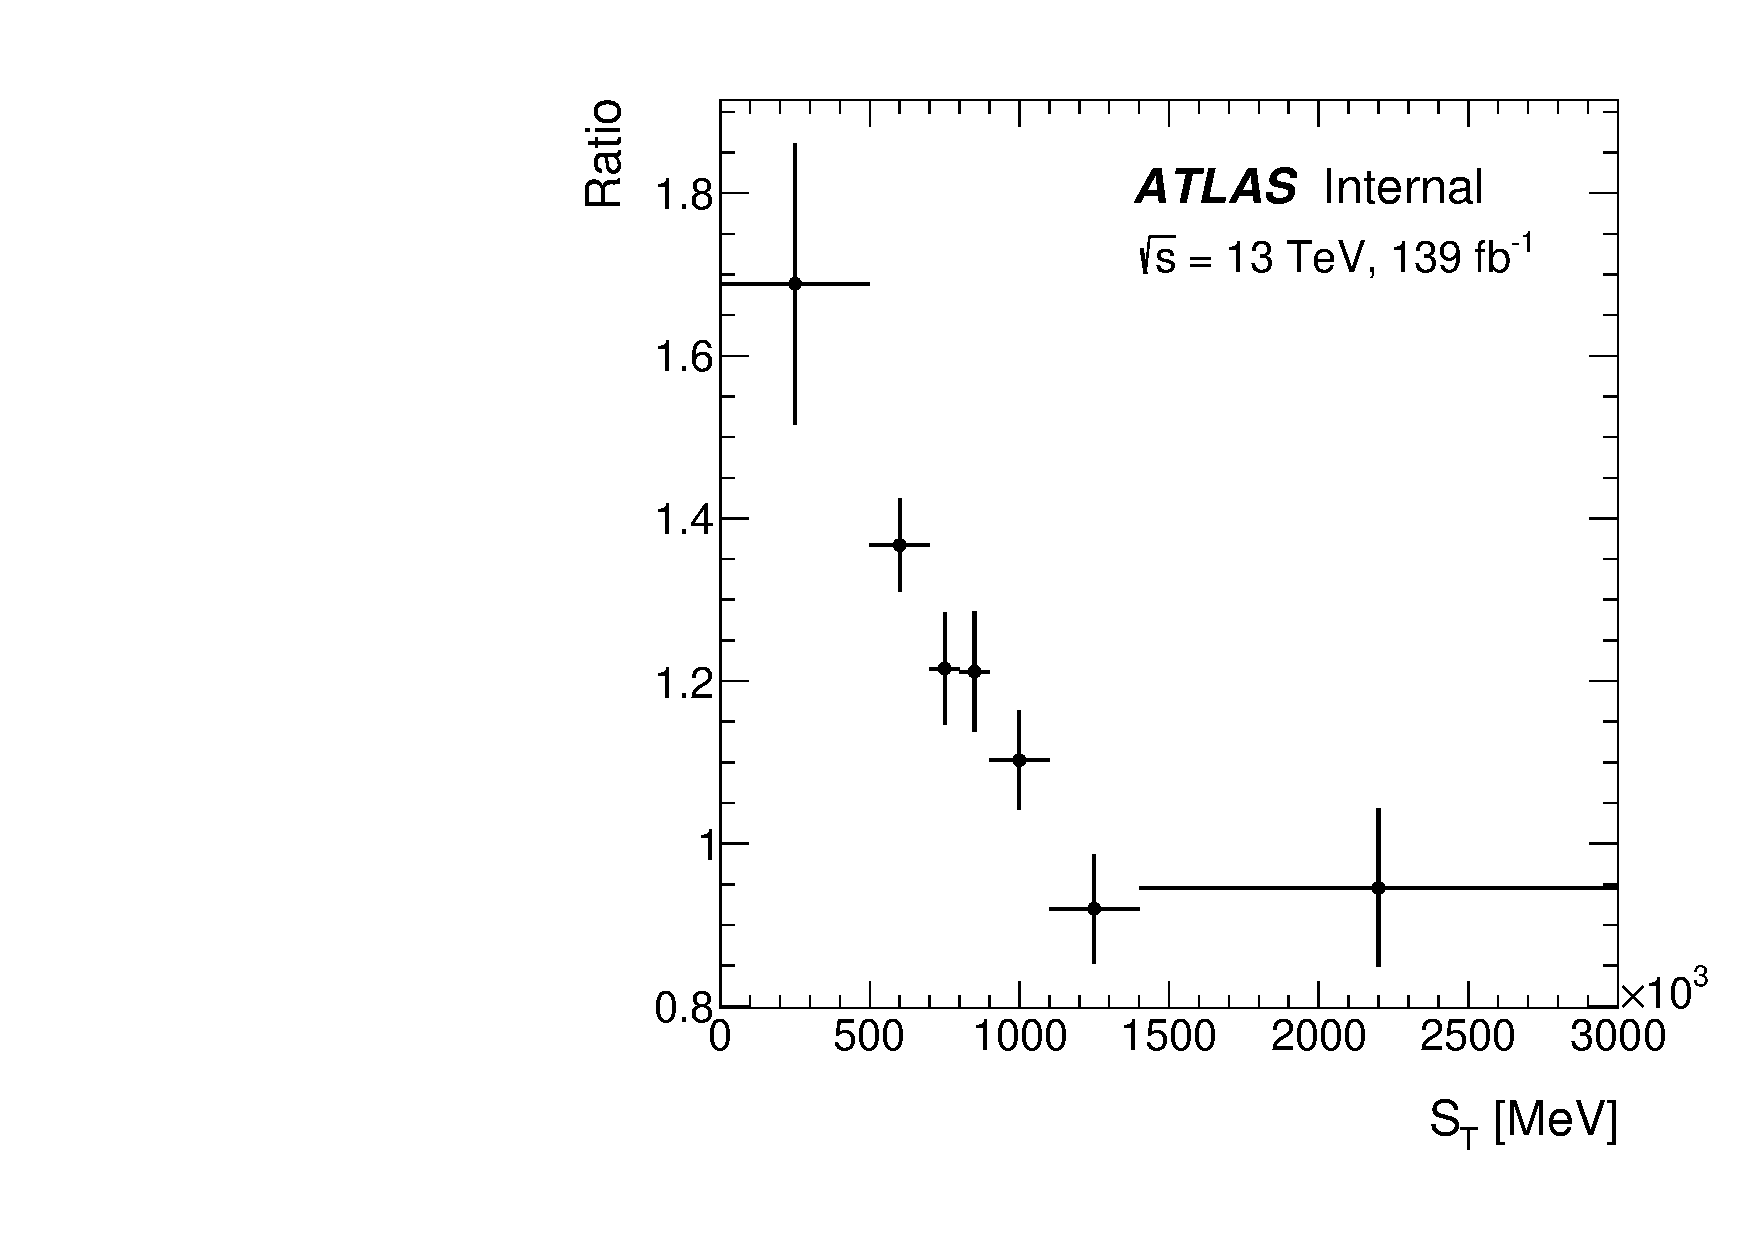
\includegraphics[width=.32\textwidth]{DiHiggs/plots/TtbarReweighting/wt1d_st_fr_os_9.pdf} }
  \subfloat[$N_{\text{jets}} \le 10$] { 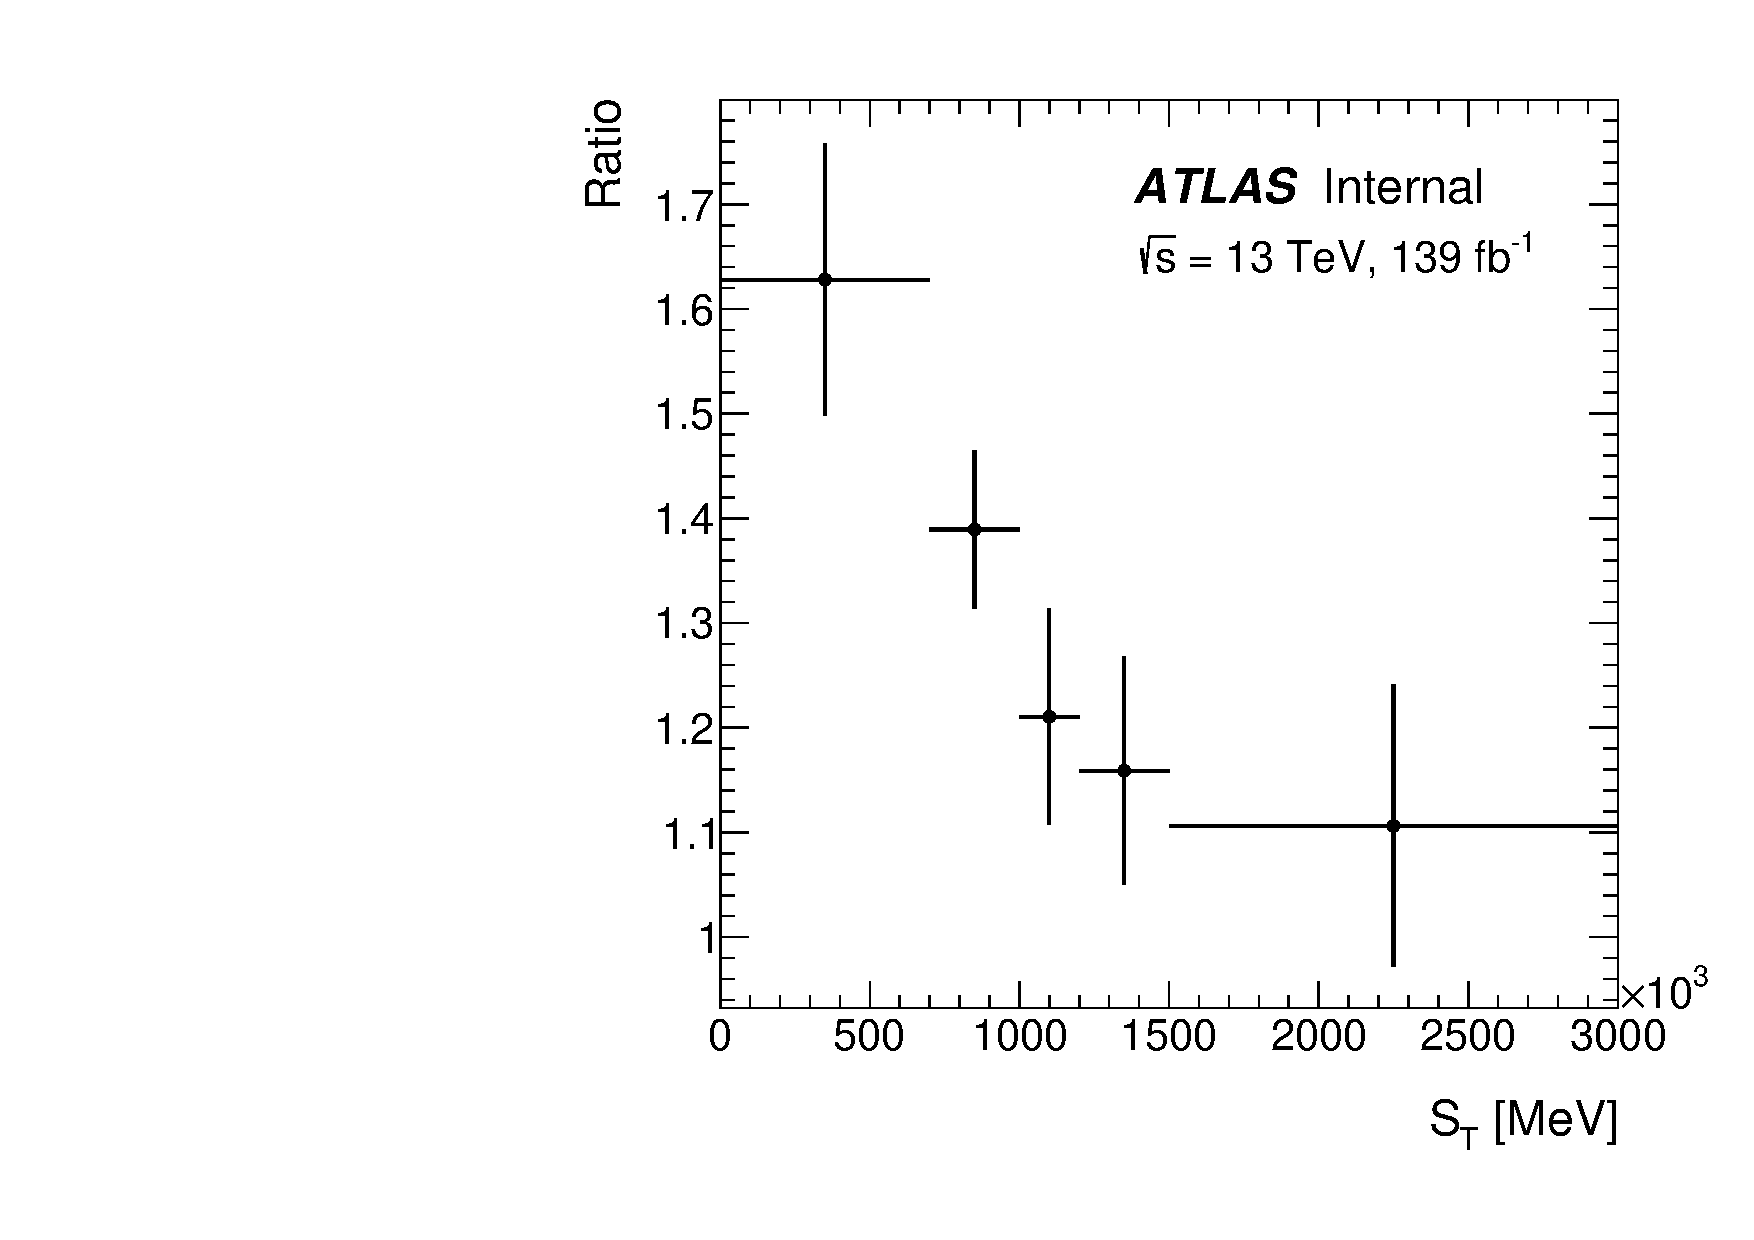
\includegraphics[width=.32\textwidth]{DiHiggs/plots/TtbarReweighting/wt1d_st_fr_os_10.pdf} }
  \caption{The \ttbar shape correction scale factor as functions of $H_{\text{T}}$ in different $N_{\text{jets}}$. 
  The error bars are calculated from the statistical uncertainties of data and simulated samples.
  Figures reproduced from analysis internal notes.}
  \label{fig:ttbarReweighting_parametrisations}
\end{figure}







\section{Additional material for MVA signal extraction}
\label{sec:appendix:mva}

The folloing figures are additional material for the MVA section.
\begin{figure}
    \centering
    \subfloat[]{\includegraphics[width=.45\textwidth]{diHiggs/plots/MVA/LephadOvertrainingPlots_10May21/SLT/NR/All/PNN.pdf}}\quad
    \subfloat[]{\includegraphics[width=.45\textwidth]{diHiggs/plots/MVA/LephadOvertrainingPlots_10May21/SLT/300/All/PNN300.pdf}}\quad\\
    \subfloat[]{\includegraphics[width=.45\textwidth]{diHiggs/plots/MVA/LephadOvertrainingPlots_10May21/SLT/500/All/PNN500.pdf}}\quad
    \subfloat[]{\includegraphics[width=.45\textwidth]{diHiggs/plots/MVA/LephadOvertrainingPlots_10May21/SLT/1000/All/PNN1000.pdf}}\quad
    \caption{(P)NN output distributions for (a) non-resonant signal, 
    and target signal masses of (b) 300~GeV, (c) 500~GeV, 
    and (d) 1000~GeV obtained evaluating the MVA with even-odd 
    events crossing or evaluating the MVA on the training datasets for the SLT category. 
    The ``OT'' histograms refer to the ``OverTraining'' check in 
    which the (P)NN is applied to the same data on which it was trained, 
    the other histograms are obtained evaluating the MVA with even-odd event crossing.
    Images reproced from analysis internal notes.}
    \label{fig:overfittingtestSLT}
  \end{figure}
  
  \begin{figure}
    \centering
    \subfloat[]{\includegraphics[width=.45\textwidth]{diHiggs/plots/MVA/LephadOvertrainingPlots_10May21/LTT/NR/All/PNN.pdf}}\quad
    \subfloat[]{\includegraphics[width=.45\textwidth]{diHiggs/plots/MVA/LephadOvertrainingPlots_10May21/LTT/300/All/PNN300.pdf}}\quad\\
    \subfloat[]{\includegraphics[width=.45\textwidth]{diHiggs/plots/MVA/LephadOvertrainingPlots_10May21/LTT/500/All/PNN500.pdf}}\quad
    \subfloat[]{\includegraphics[width=.45\textwidth]{diHiggs/plots/MVA/LephadOvertrainingPlots_10May21/LTT/1000/All/PNN1000.pdf}}\quad
    \caption{(P)NN output distributions for 
    (a) non-resonant signal, and target signal masses of 
    (b) 300~GeV, (c) 500~GeV, and (d) 1000~GeV obtained 
    evaluating the MVA with even-odd events crossing or 
    evaluating the MVA on the training datasets for the LTT category. 
    The ``OT'' histograms refer to the ``OverTraining'' check in which 
    the (P)NN is applied to the same data on which it was trained, 
    the other histograms are obtained evaluating the MVA with even-odd event crossing.
    Images reproced from analysis internal notes.}
    \label{fig:overfittingtestLTT}
  \end{figure}

  \begin{figure}
    \centering
    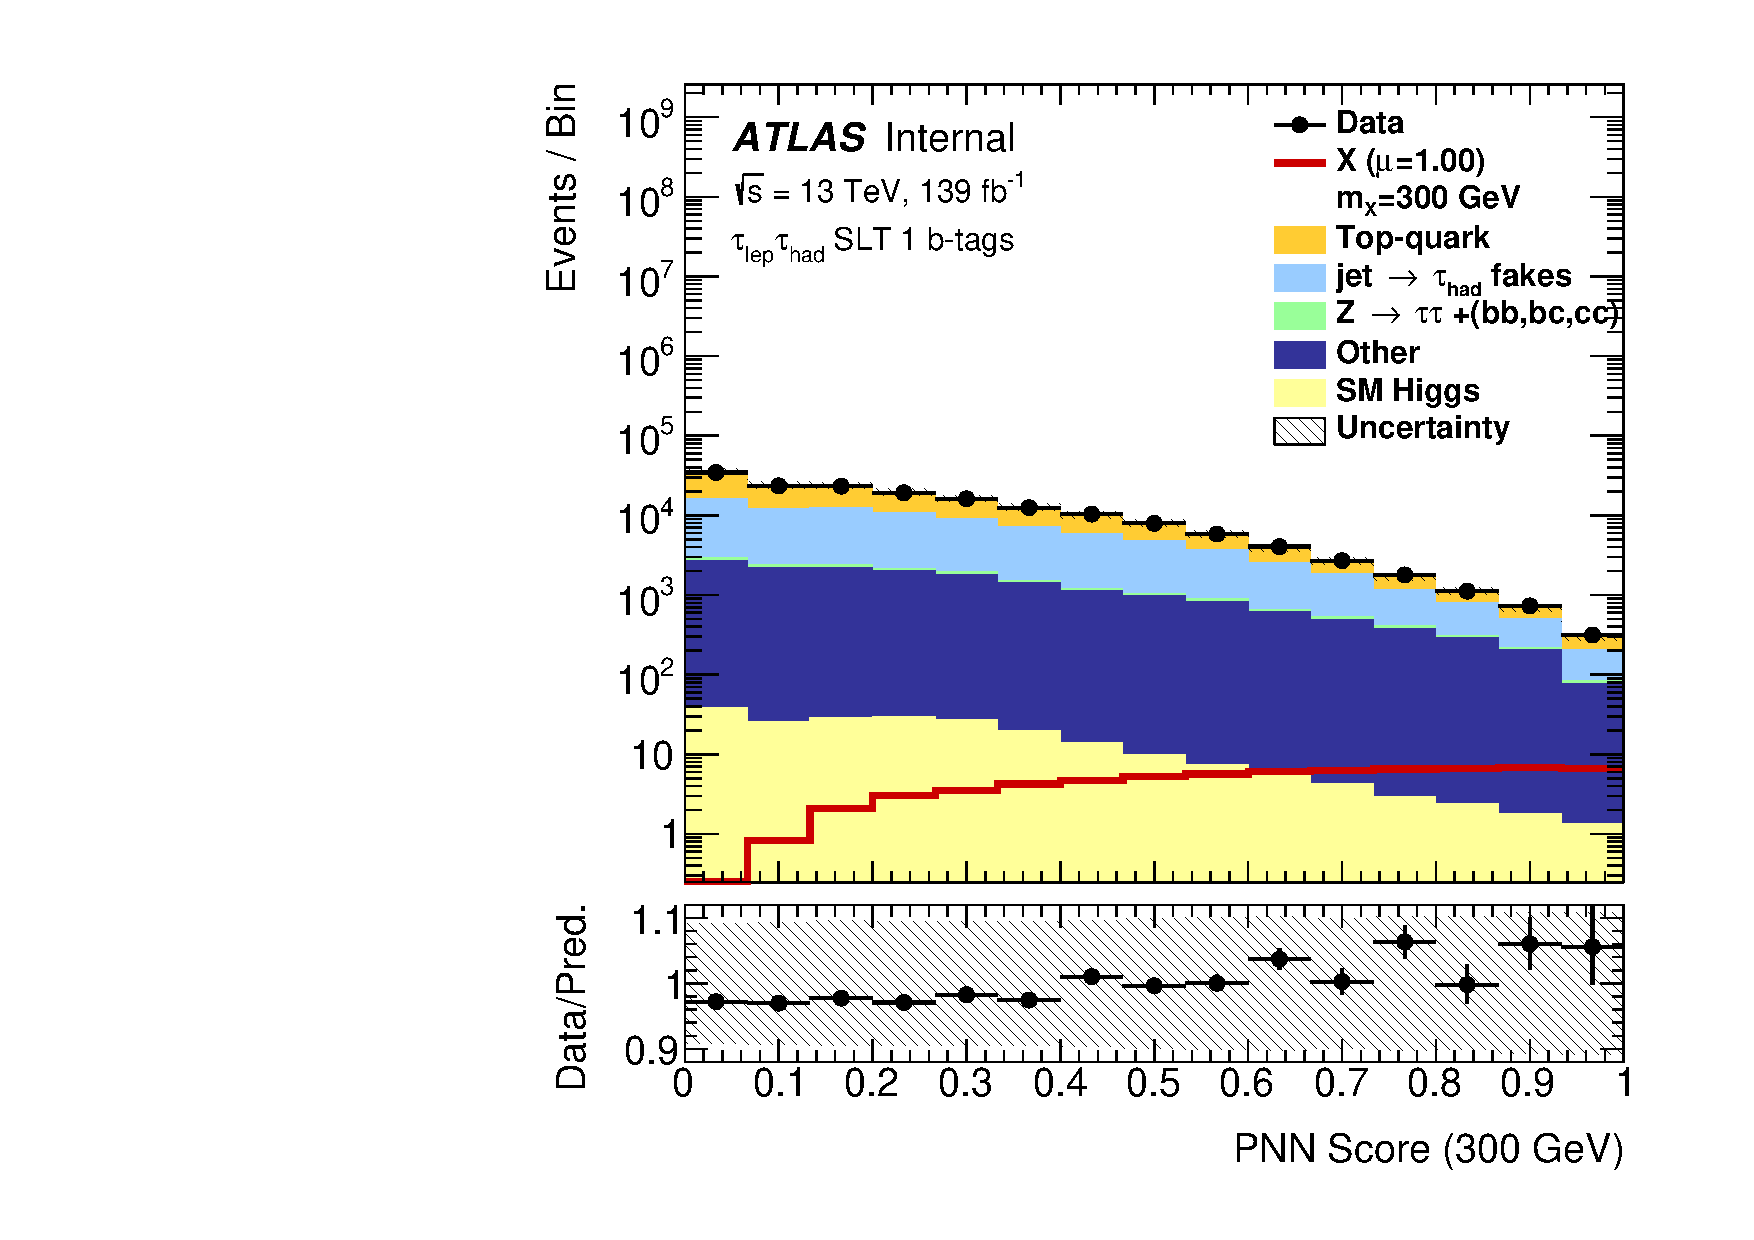
\includegraphics[width=.32\textwidth]{DiHiggs/plots/MVA/SLT/Region_BMin0_incJet1_dist300_J2_D2HDMPNN_T1_SpcTauLH_Y2015_LTT0_L1_Prefitlog.pdf}
    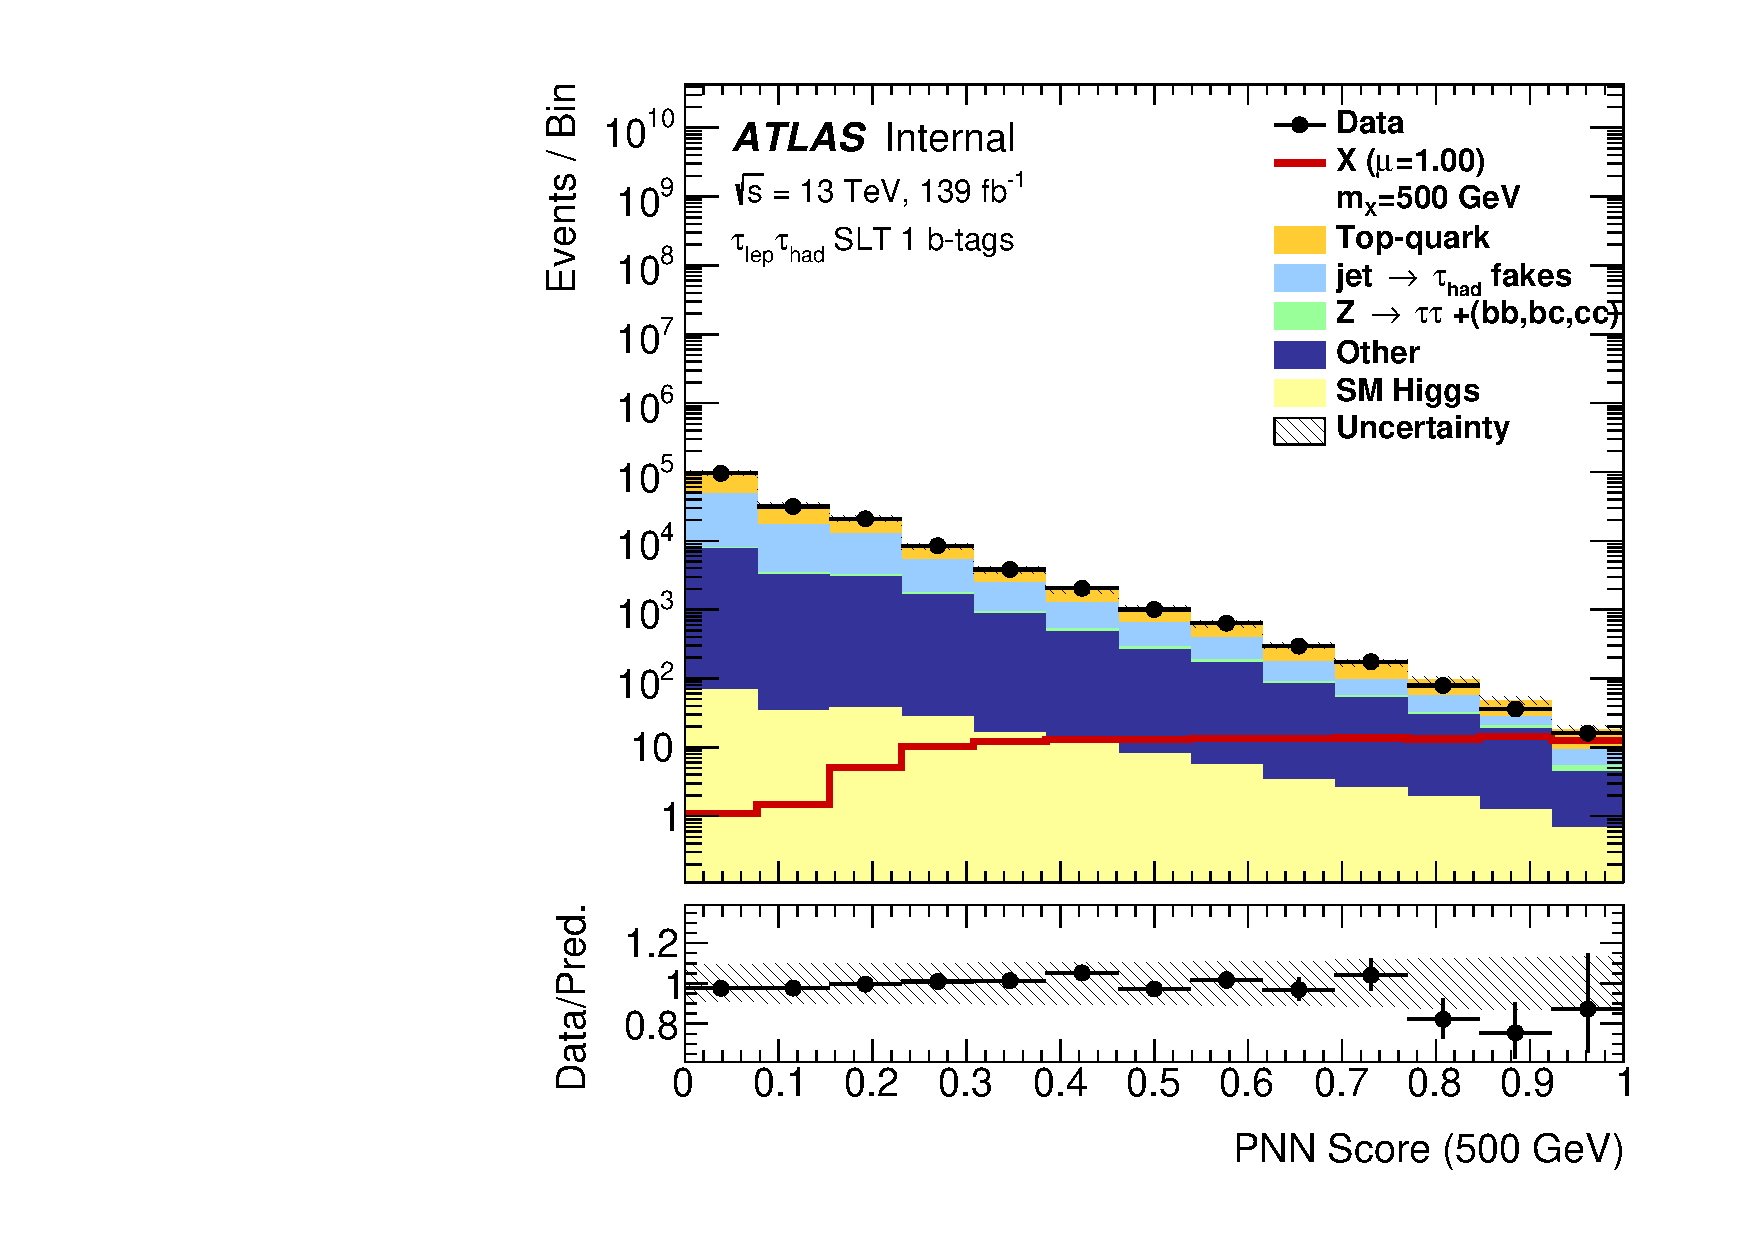
\includegraphics[width=.32\textwidth]{DiHiggs/plots/MVA/SLT/Region_BMin0_incJet1_dist500_J2_D2HDMPNN_T1_SpcTauLH_Y2015_LTT0_L1_Prefitlog.pdf}
    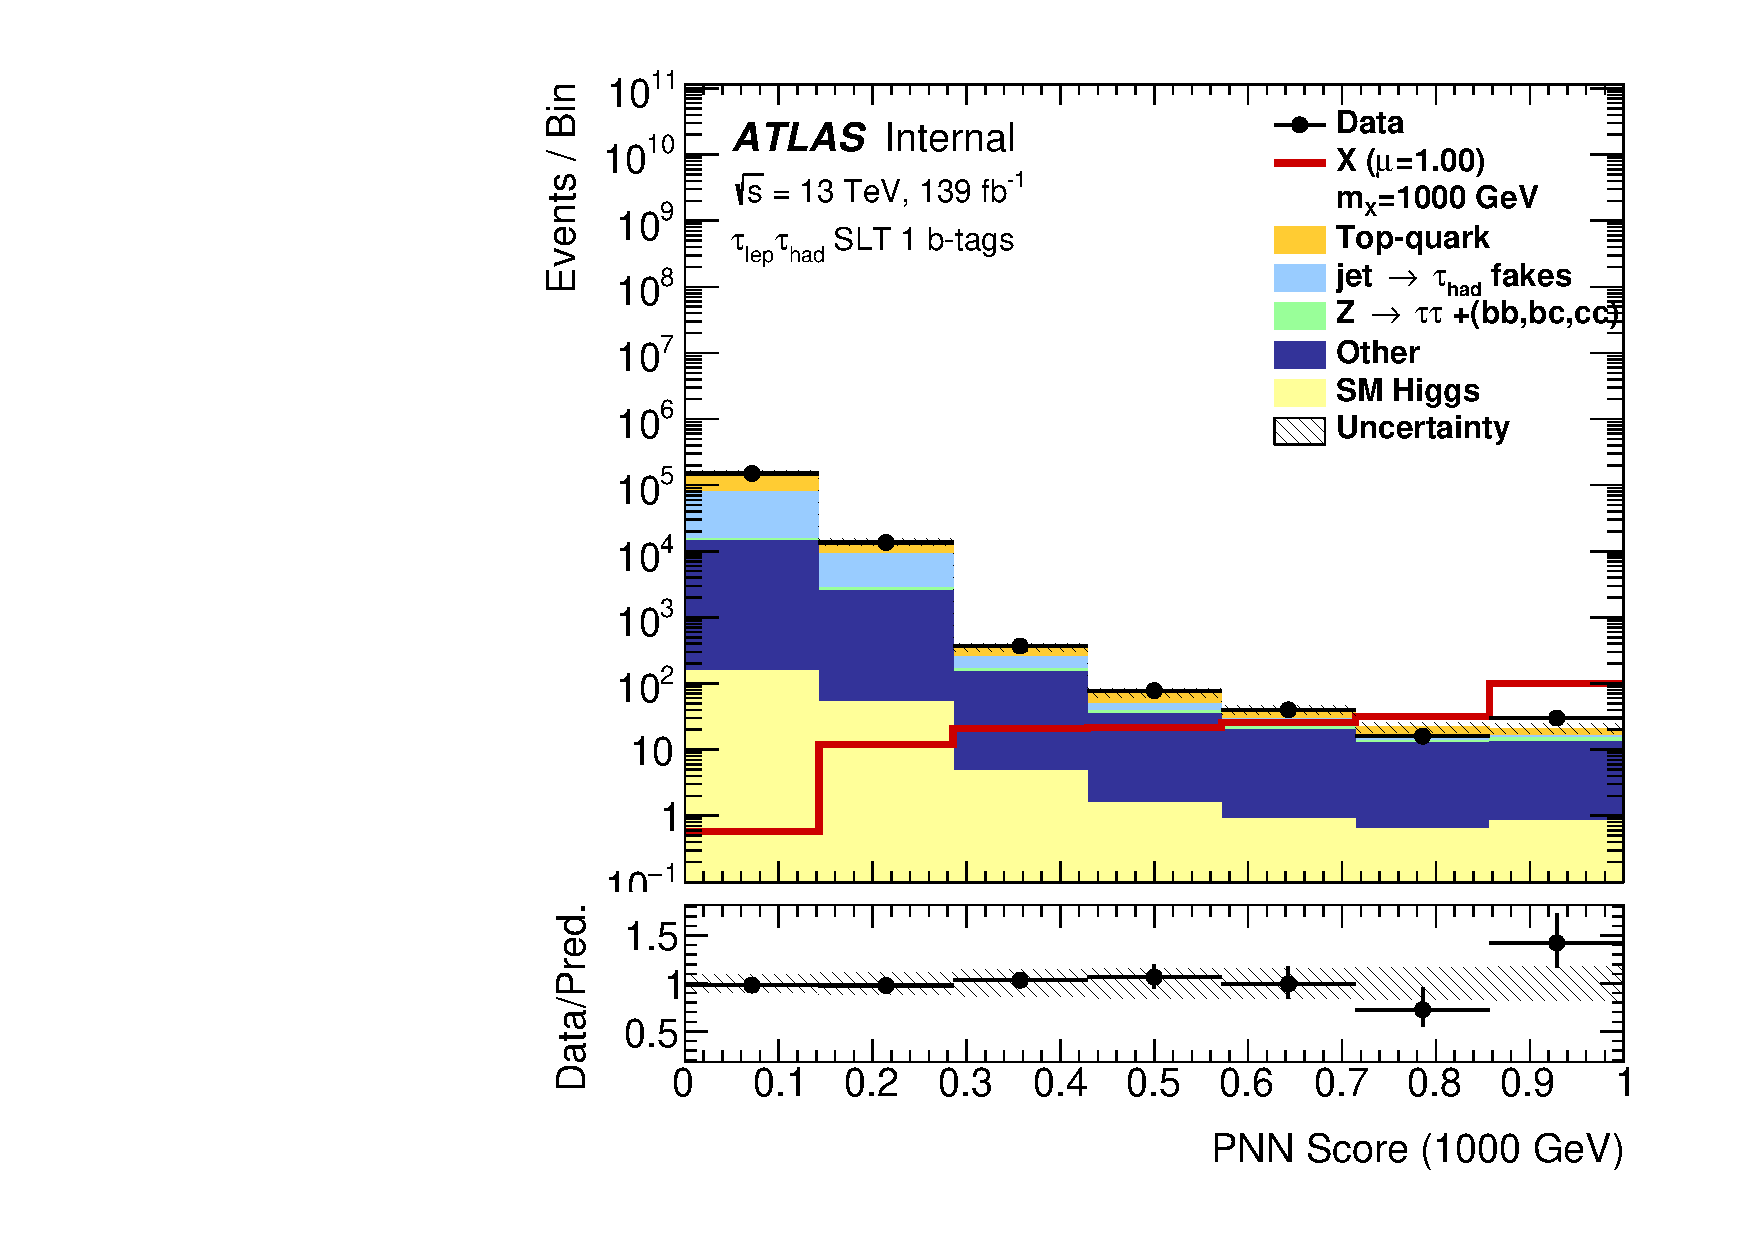
\includegraphics[width=.32\textwidth]{DiHiggs/plots/MVA/SLT/Region_BMin0_incJet1_dist1000_J2_D2HDMPNN_T1_SpcTauLH_Y2015_LTT0_L1_Prefitlog.pdf} \\
    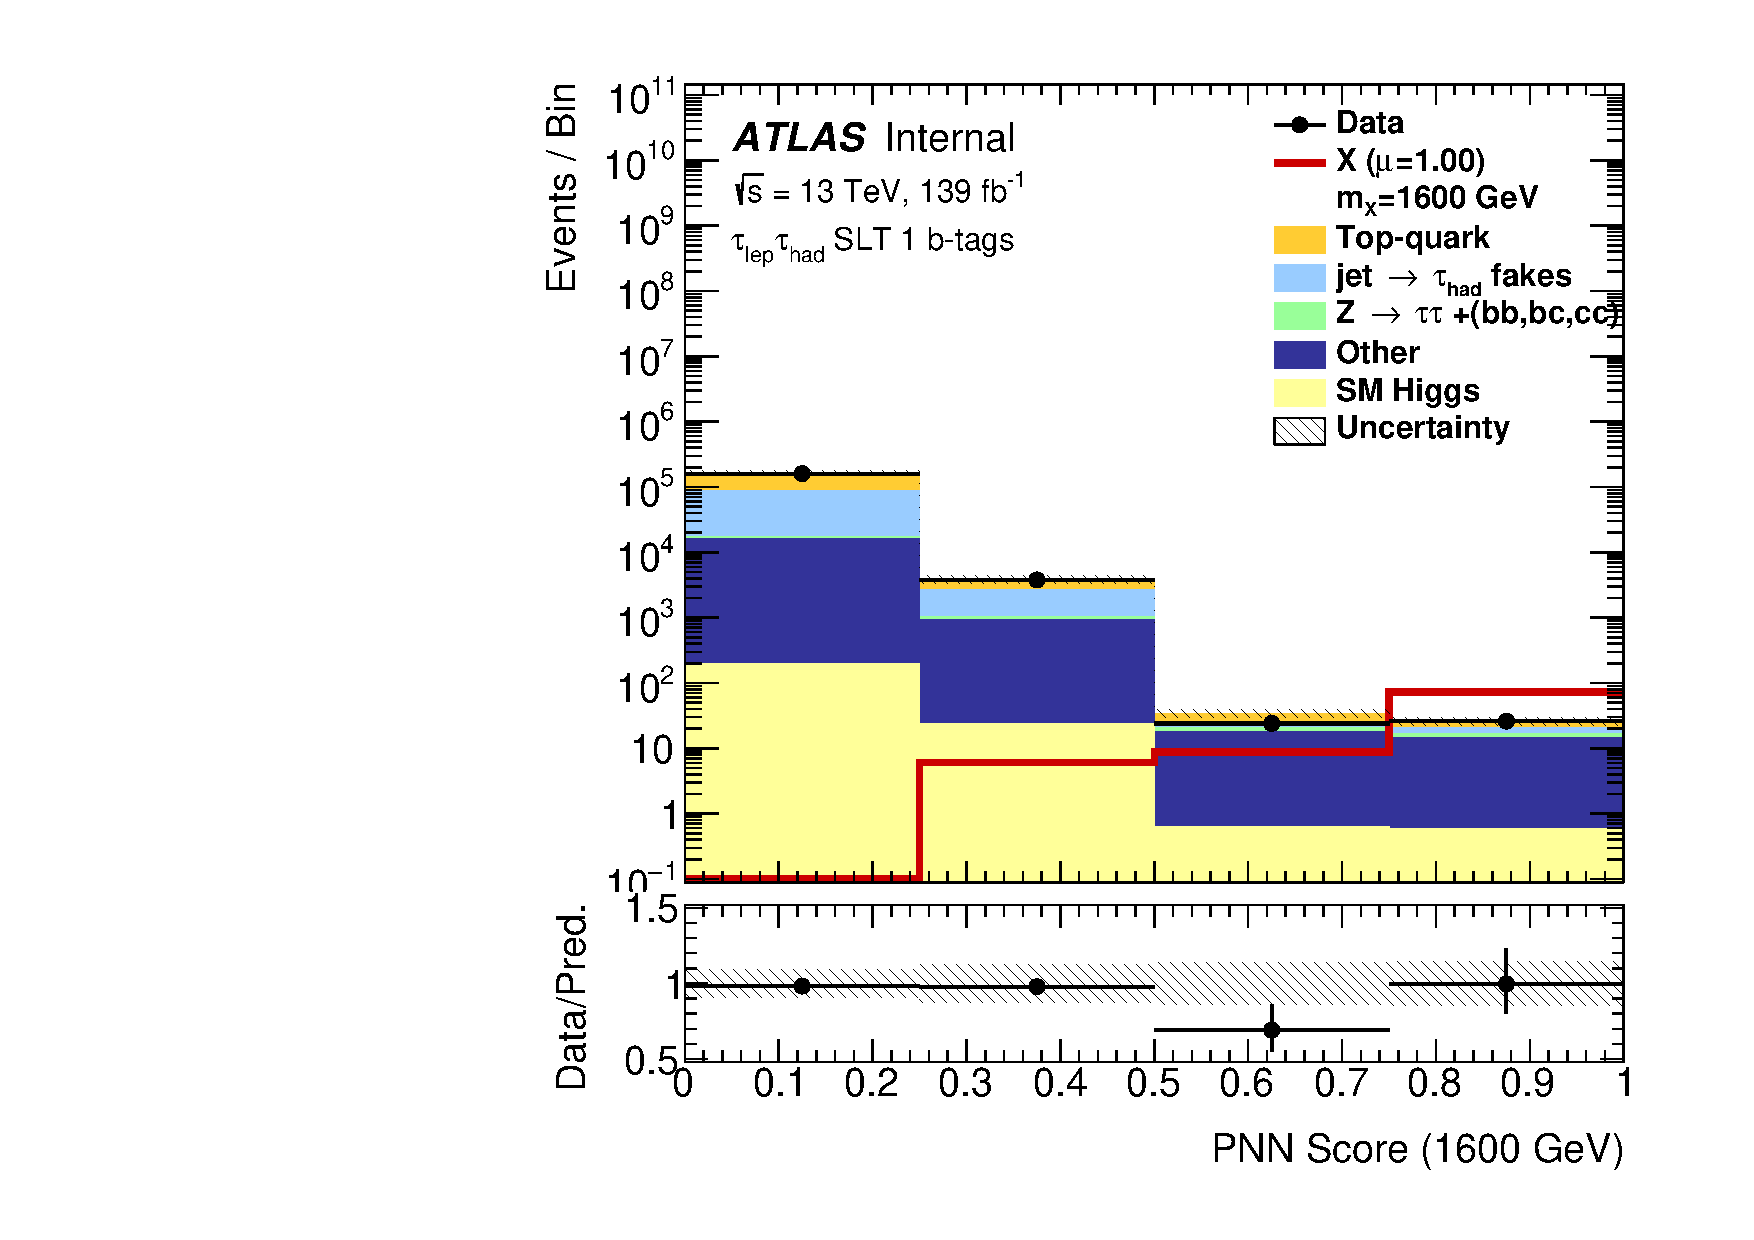
\includegraphics[width=.32\textwidth]{DiHiggs/plots/MVA/SLT/Region_BMin0_incJet1_dist1600_J2_D2HDMPNN_T1_SpcTauLH_Y2015_LTT0_L1_Prefitlog.pdf}
    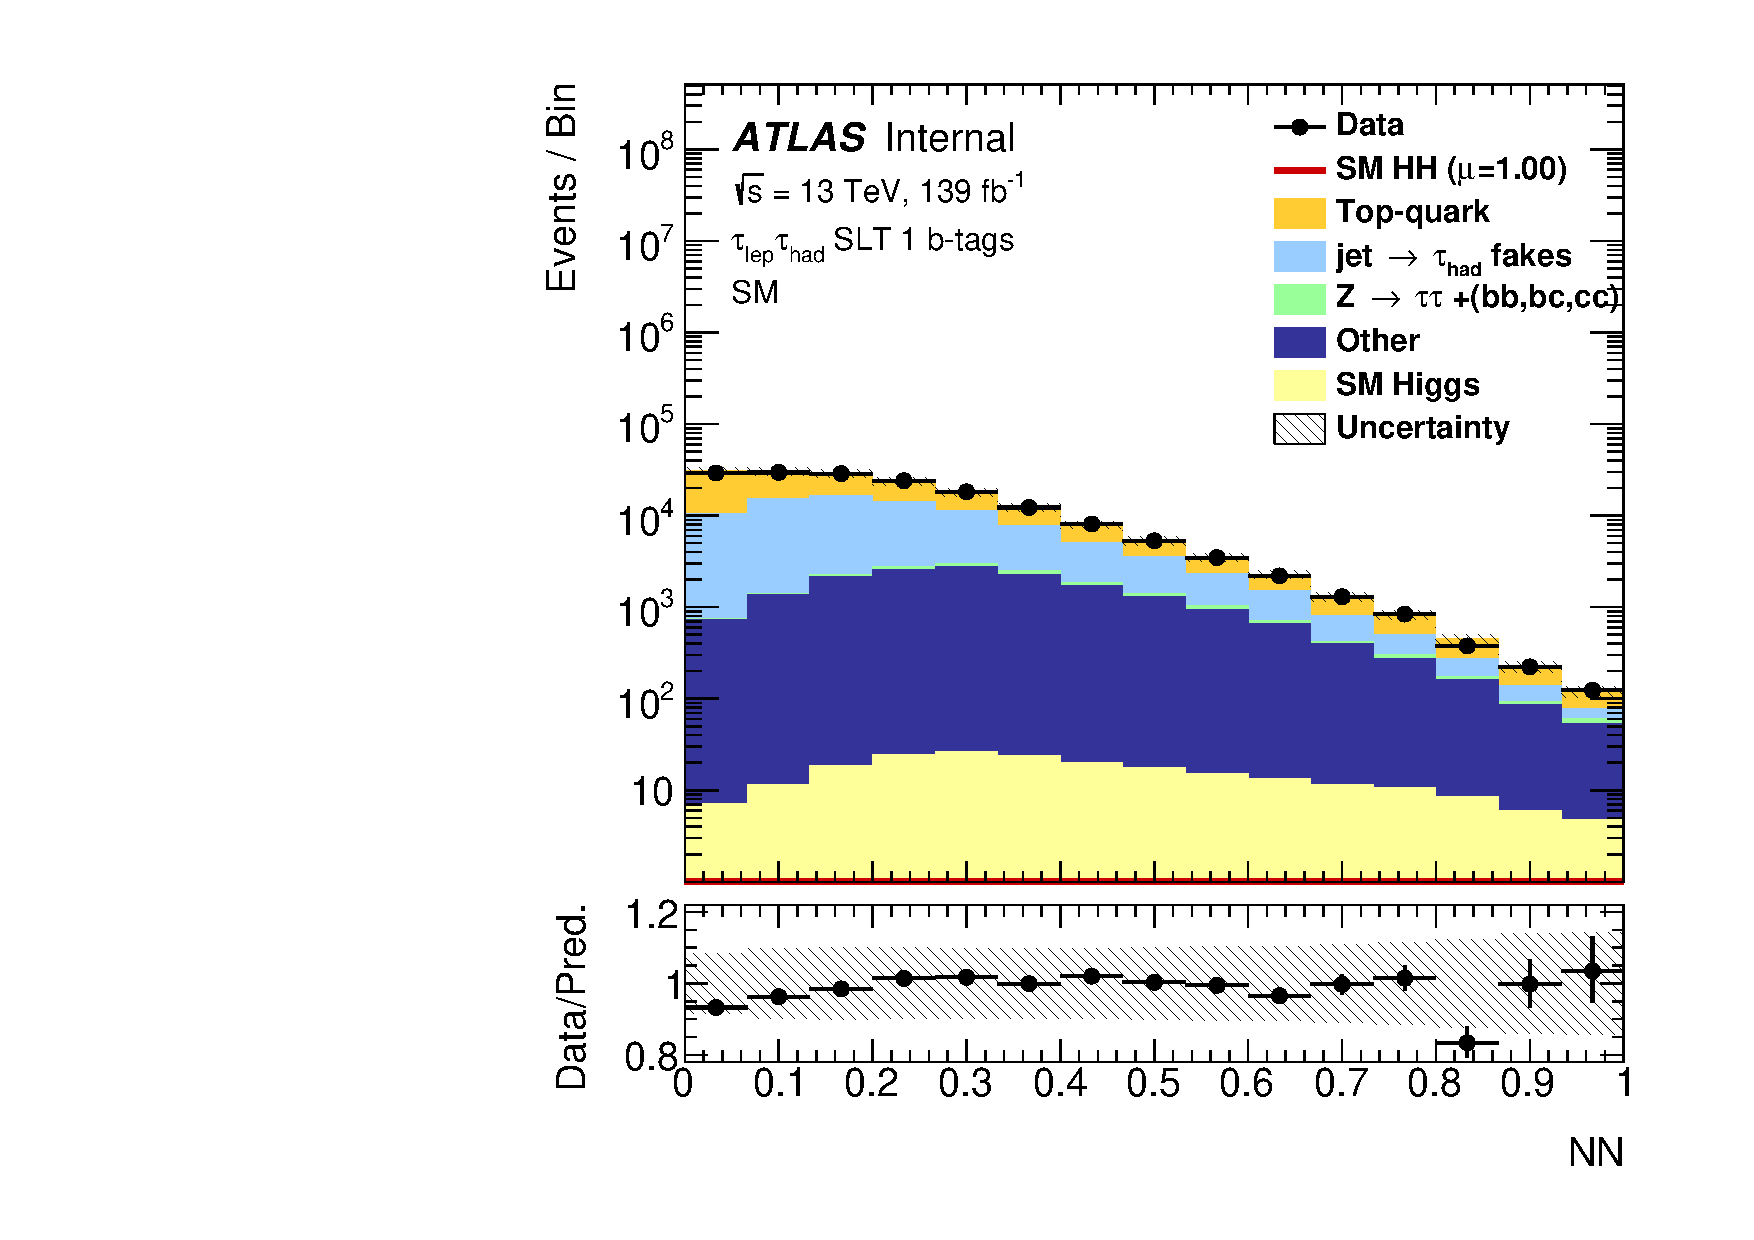
\includegraphics[width=.32\textwidth]{DiHiggs/plots/MVA/SLT/Region_BMin0_incJet1_distNN_J2_DSM_T1_SpcTauLH_Y2015_LTT0_L1_Prefitlog.pdf} \\
    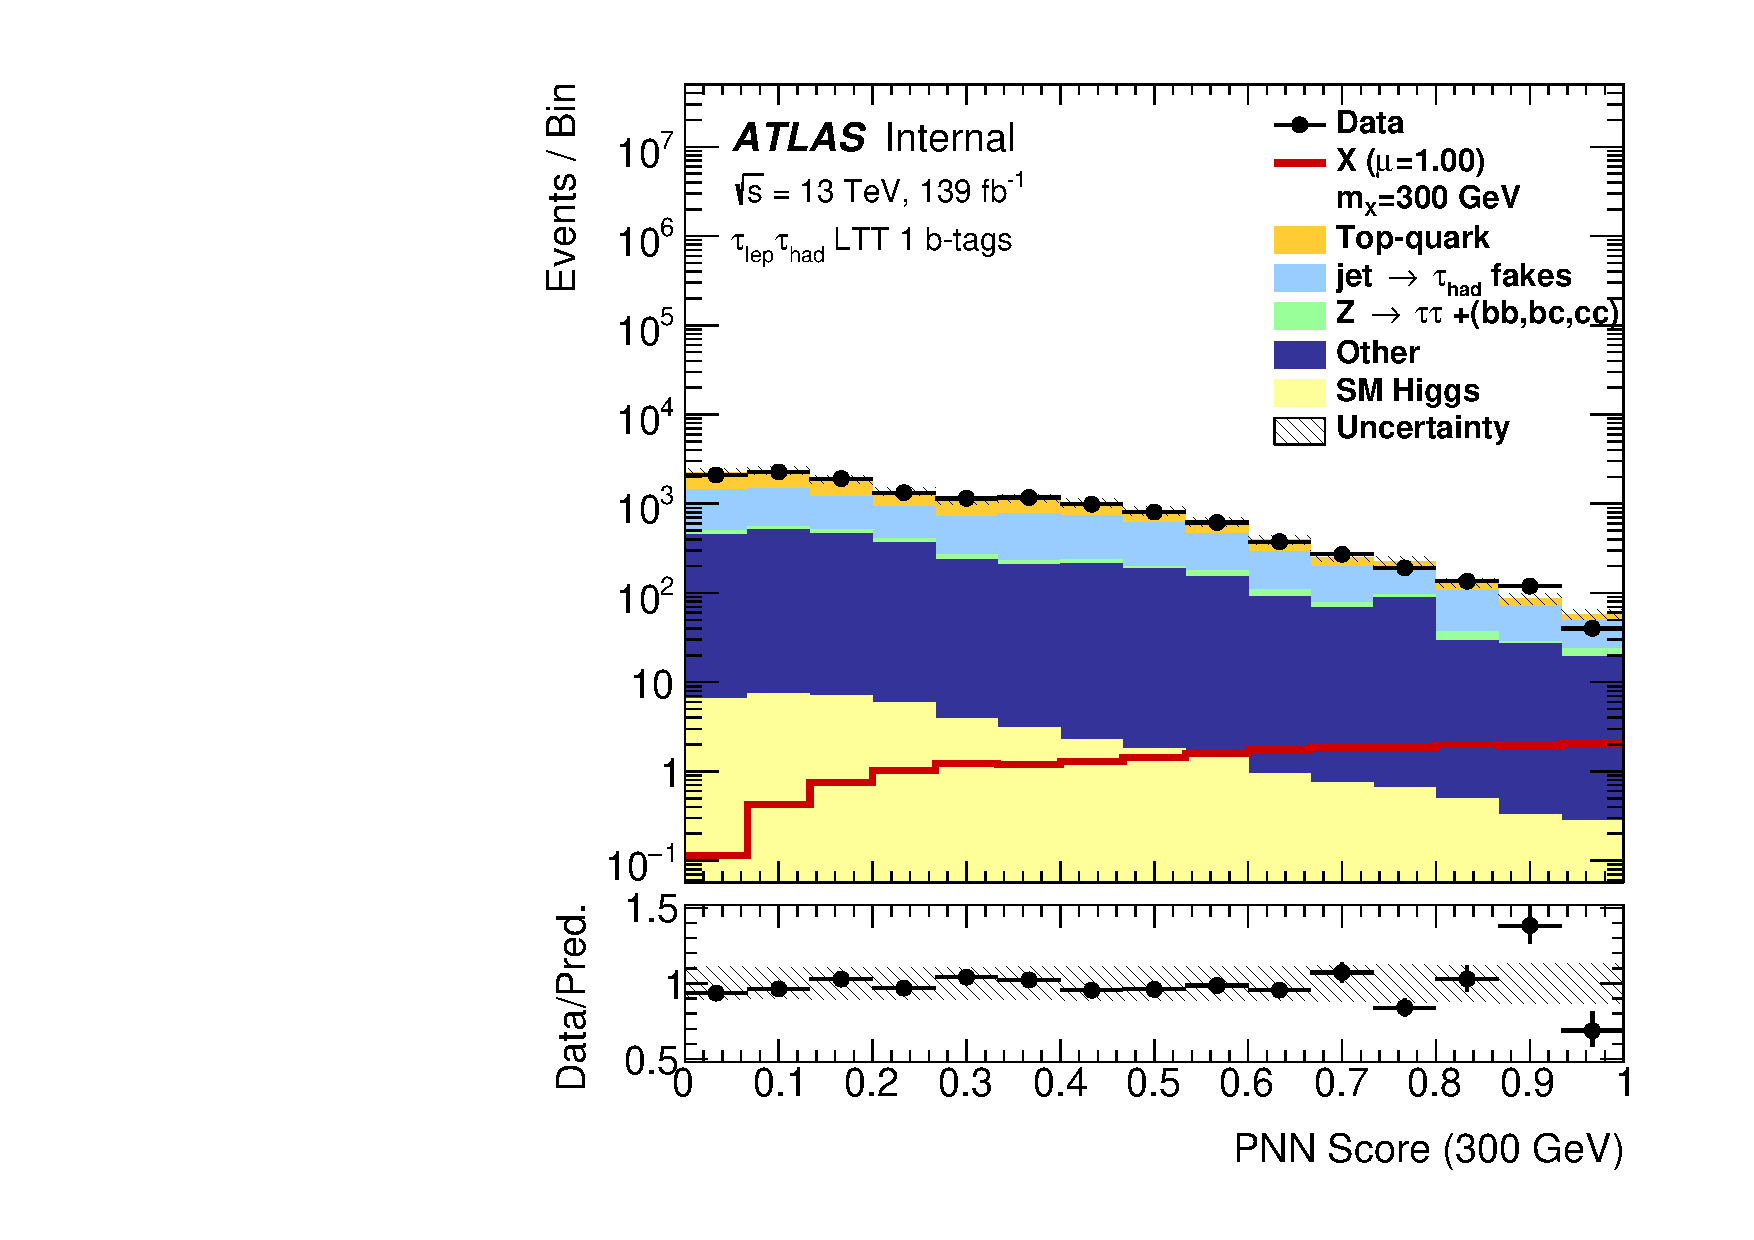
\includegraphics[width=.32\textwidth]{DiHiggs/plots/MVA/LTT/Region_BMin0_incJet1_dist300_J2_D2HDMPNN_T1_SpcTauLH_Y2015_LTT1_L1_Prefitlog.pdf}
    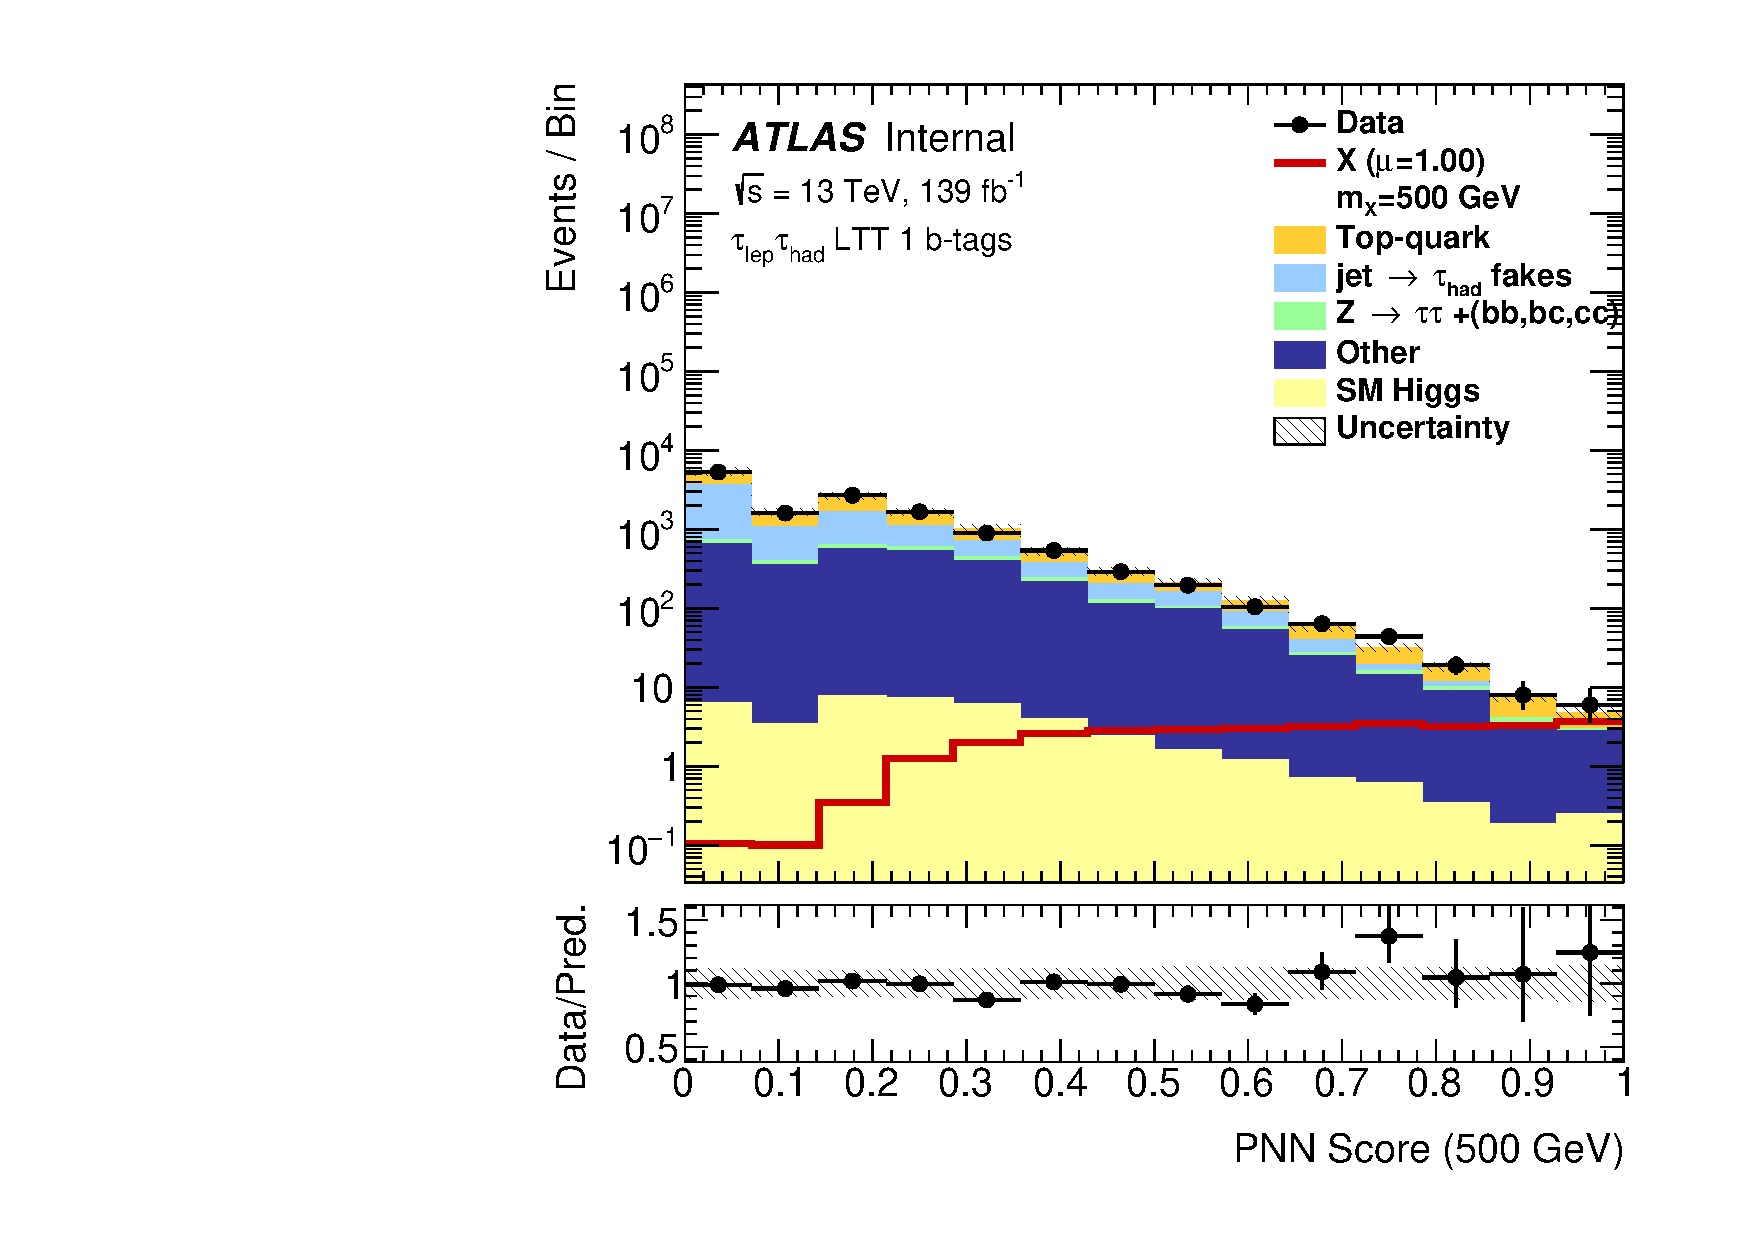
\includegraphics[width=.32\textwidth]{DiHiggs/plots/MVA/LTT/Region_BMin0_incJet1_dist500_J2_D2HDMPNN_T1_SpcTauLH_Y2015_LTT1_L1_Prefitlog.pdf}
    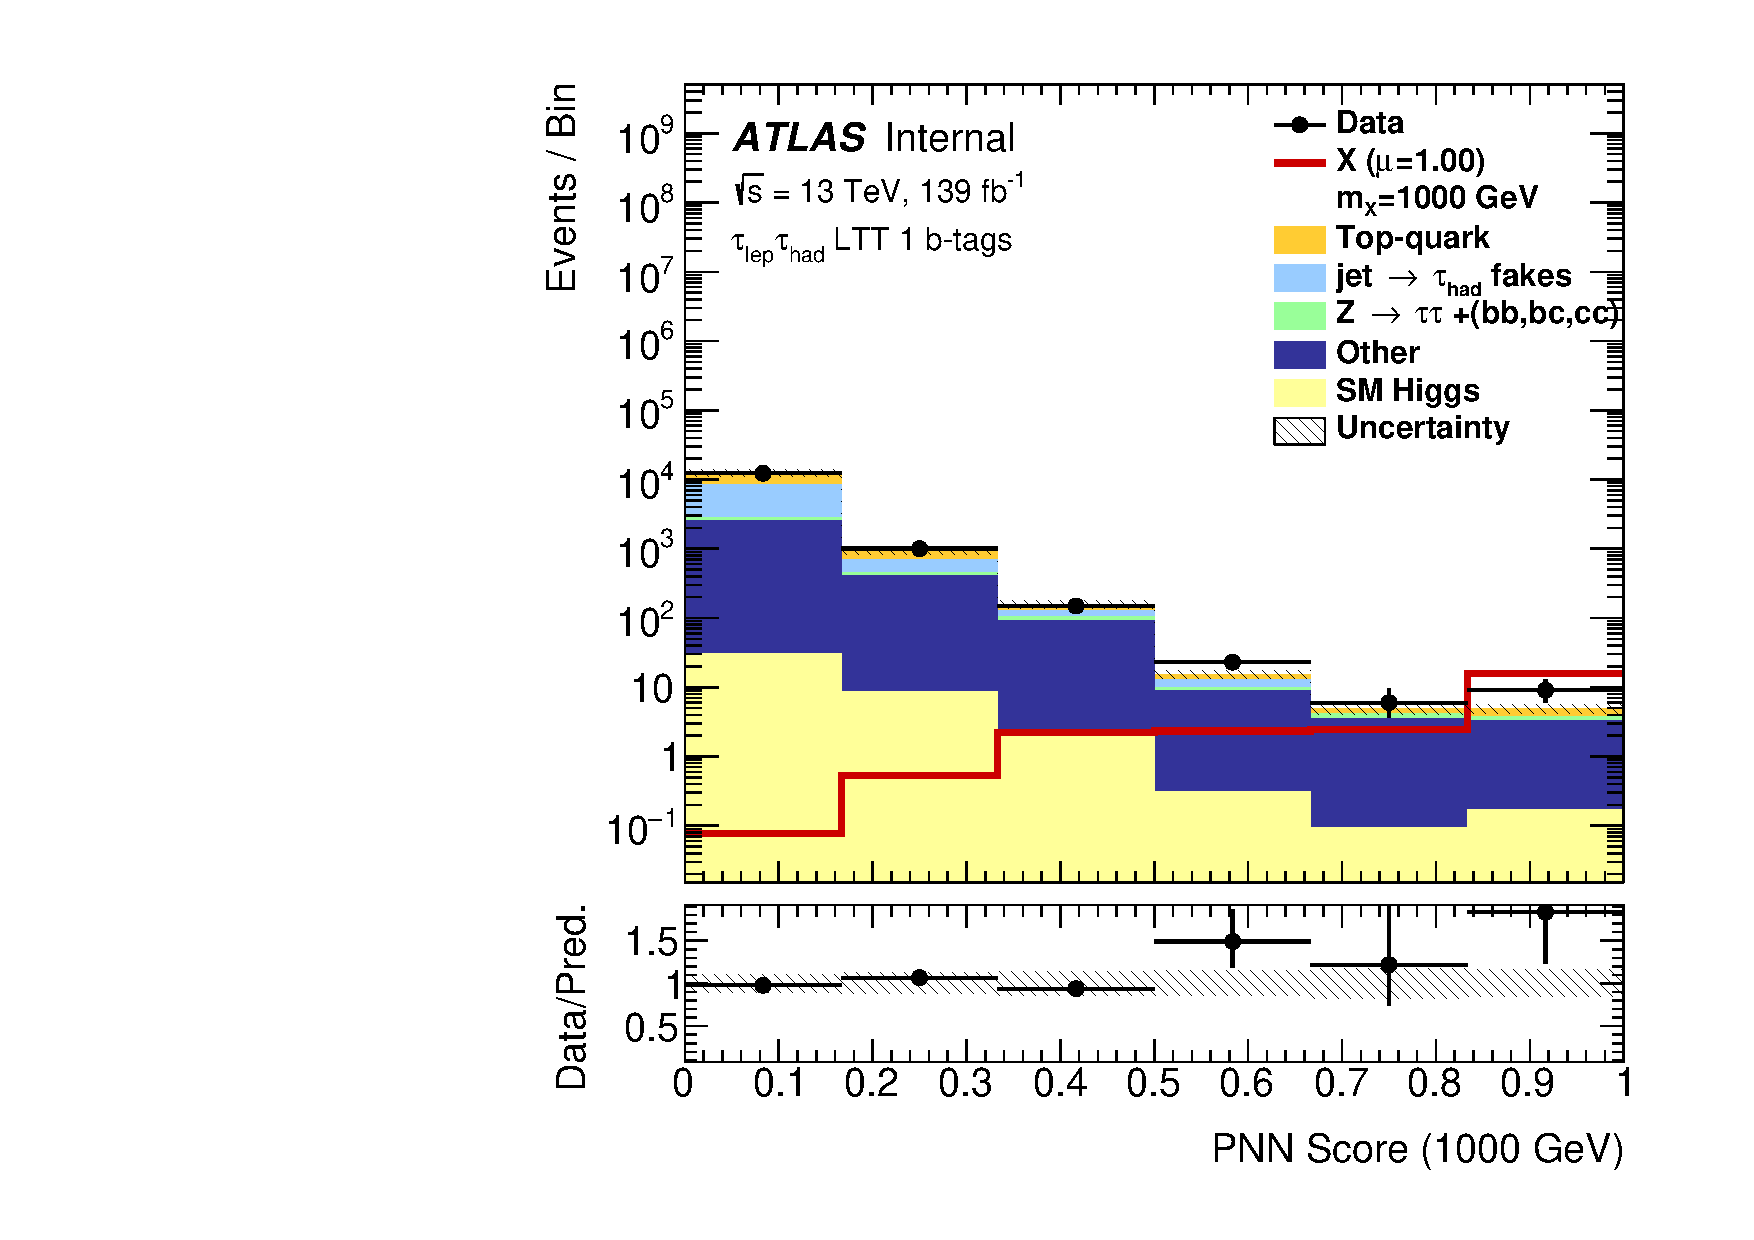
\includegraphics[width=.32\textwidth]{DiHiggs/plots/MVA/LTT/Region_BMin0_incJet1_dist1000_J2_D2HDMPNN_T1_SpcTauLH_Y2015_LTT1_L1_Prefitlog.pdf} \\
    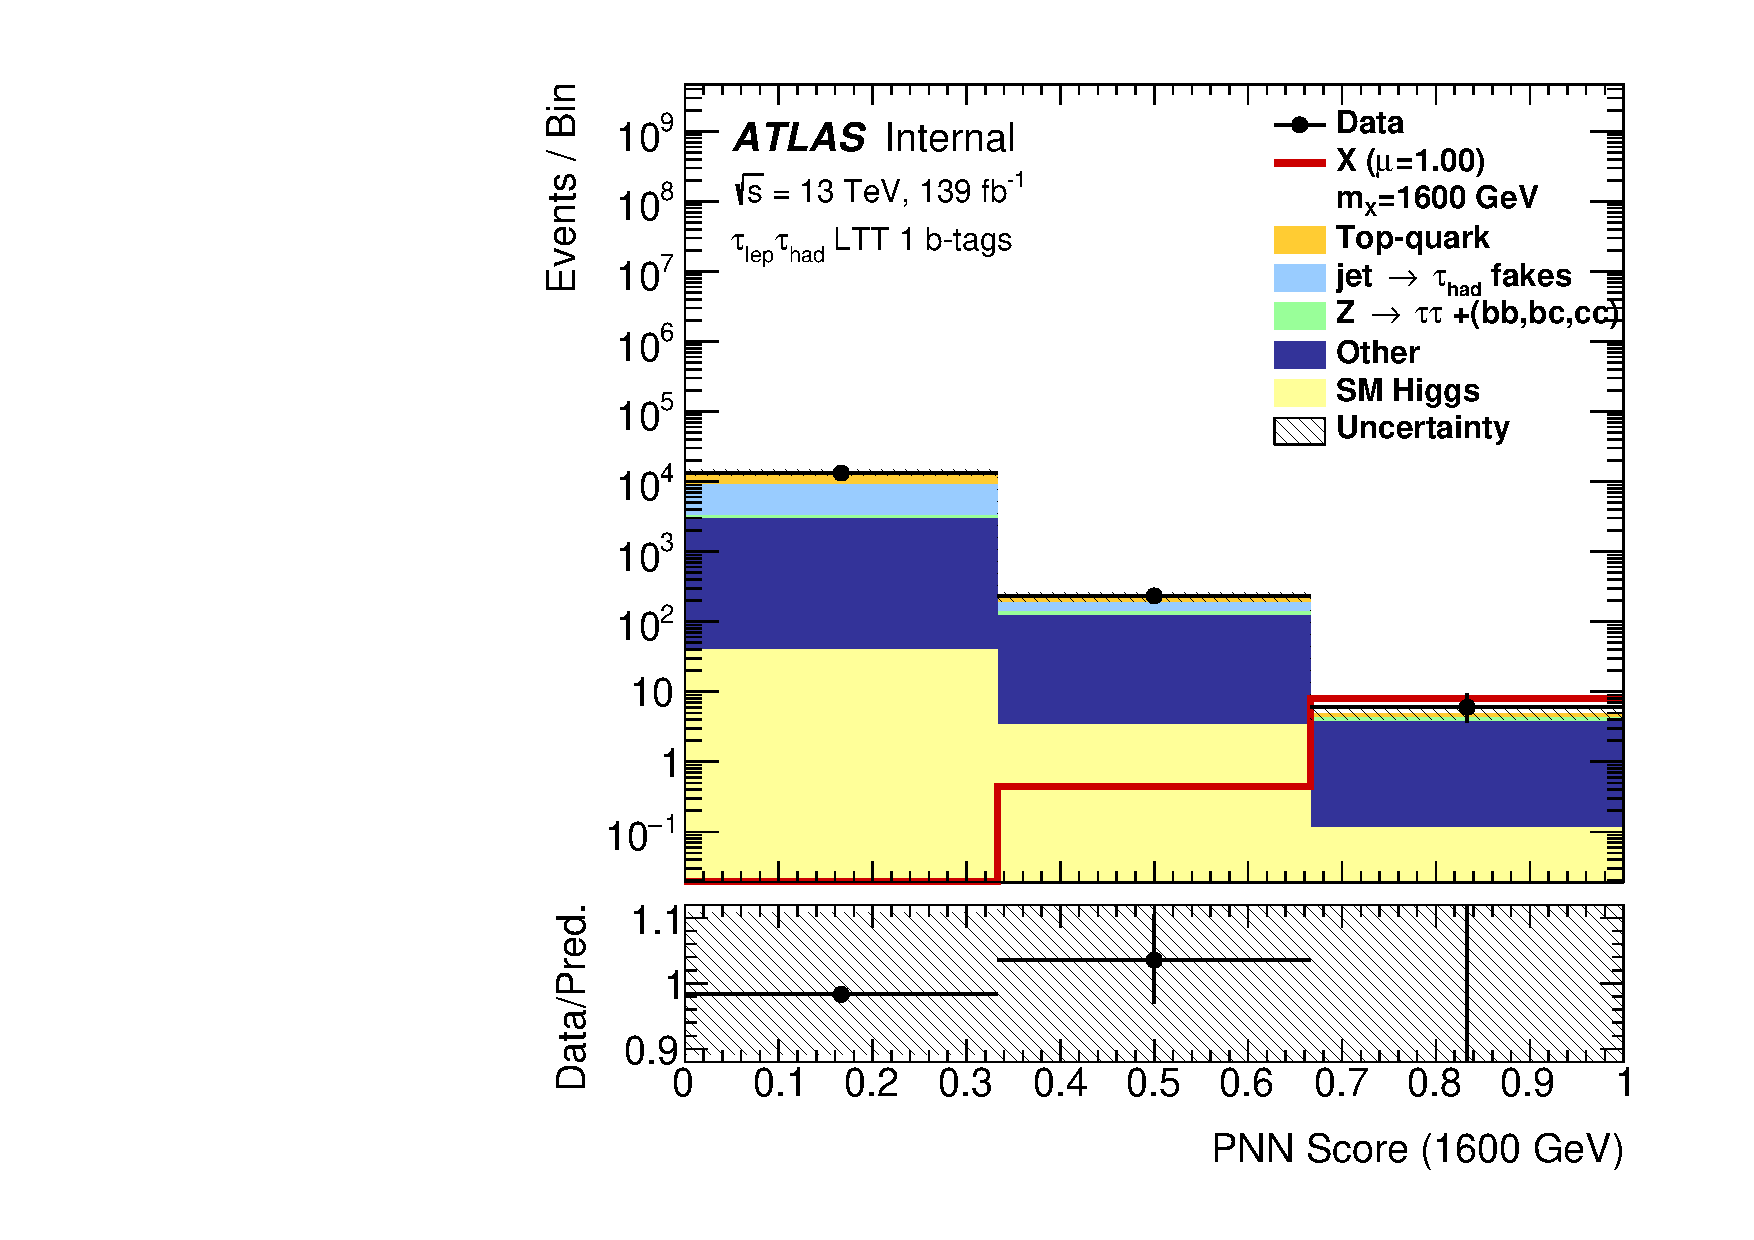
\includegraphics[width=.32\textwidth]{DiHiggs/plots/MVA/LTT/Region_BMin0_incJet1_dist1600_J2_D2HDMPNN_T1_SpcTauLH_Y2015_LTT1_L1_Prefitlog.pdf}
    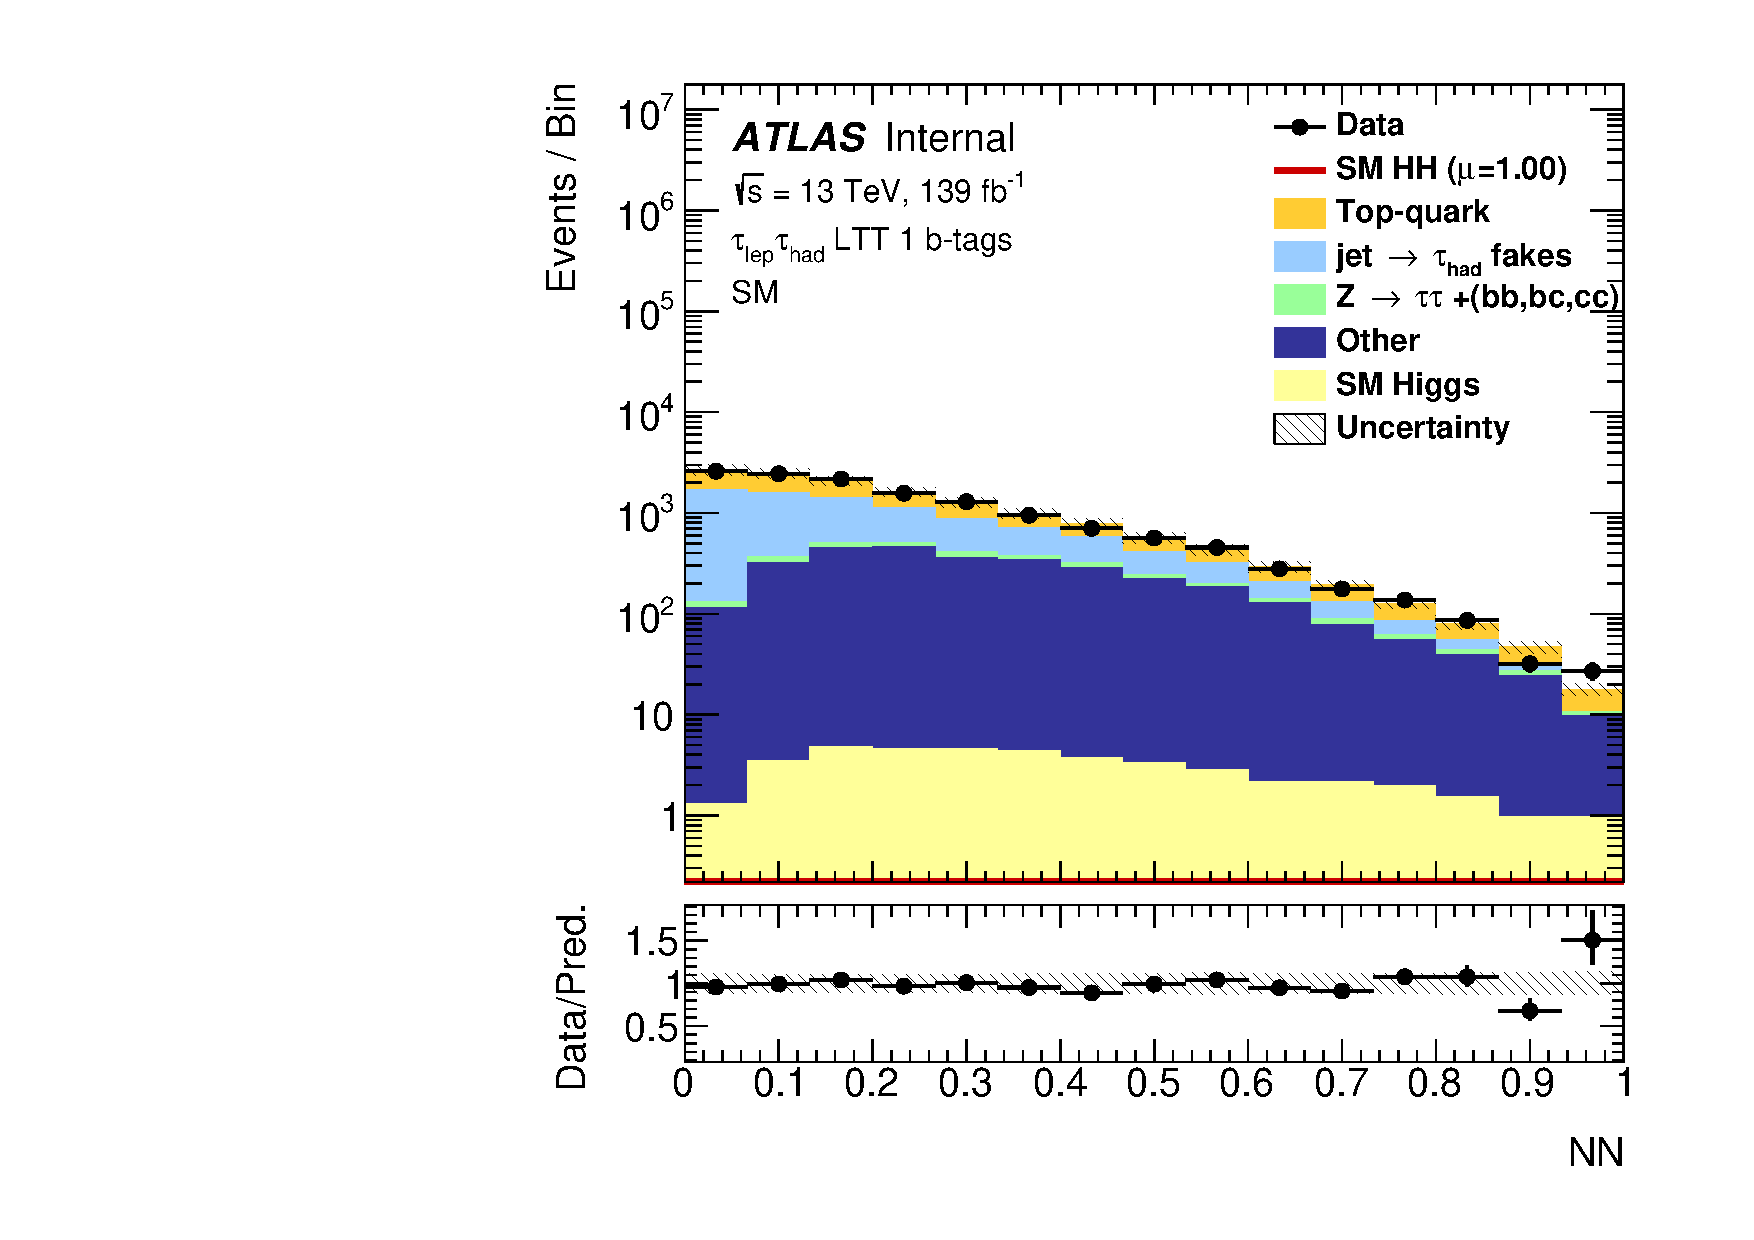
\includegraphics[width=.32\textwidth]{DiHiggs/plots/MVA/LTT/Region_BMin0_incJet1_distNN_J2_DSM_T1_SpcTauLH_Y2015_LTT1_L1_Prefitlog.pdf}
    \caption{Pre-fit PNN score distributions for the $300, 500, 1000, 1600$ 
    GeV mass points and non-resonant NN in the di-Higgs $bb\lephad$ SLT (top two rows) and LTT (bottom two rows) 1tag control regions.}
    \label{fig:lephadmvaCRoutput}
    \end{figure}


  \begin{table}
    \centering
    \footnotesize
    \begin{tabular}{|c|c|c|c|c|}
    \hline
    \multicolumn{5}{|c|}{Last bin}\\
    \hline
    Process & Last bin SM & Last bin 300 GeV & Last bin 500 GeV & Last bin 1000 GeV\\
    \hline
    ttbar &  $0.46 \pm 0.22$ &  $30.9 \pm 2$ &  $1.3 \pm 0.4$ &  $0.68 \pm 0.28$ \\
    Fake &  $1.2 \pm 0.7$ &  $16.7 \pm 2.4$ &  $1.1 \pm 0.6$ &  $0.8 \pm 0.6$ \\
    Stop &  $0.93 \pm 0.35$ &  $3 \pm 0.6$ &  $0.96 \pm 0.35$ &  $0.9 \pm 0.34$ \\
    ZHF &  $1.32 \pm 0.26$ &  $8.6 \pm 3.2$ &  $1.36 \pm 0.28$ &  $1.94 \pm 0.25$ \\
    ZLF &  $0.04 \pm 0.025$ &  $-0.25 \pm 0.25$ &  $0.029 \pm 0.029$ &  $0.27 \pm 0.18$ \\
    WHbb &  $0.0005 \pm 0.00035$ & 0 &  $0.0021 \pm 0.0012$ &  $0.0033 \pm 0.0013$ \\
    WHtautau & 0 & 0 &  $0.006 \pm 0.006$ & 0 \\
    qqZHbb &  $0.278 \pm 0.006$ &  $0.048 \pm 0.008$ &  $0.078 \pm 0.004$ &  $0.393 \pm 0.007$ \\
    ggZHbb &  $0.054 \pm 0.004$ &  $0.0008 \pm 0.0005$ &  $0.09 \pm 0.05$ &  $0.0342 \pm 0.0034$ \\
    qqZHtautau &  $0.28 \pm 0.04$ &  $0.059 \pm 0.016$ &  $0.084 \pm 0.023$ &  $0.158 \pm 0.028$ \\
    ggZHtautau &  $0.052 \pm 0.014$ &  $0.00016 \pm 0.00016$ &  $0.061 \pm 0.015$ &  $0.032 \pm 0.011$ \\
    ggFHtautau &  $0.25 \pm 0.05$ & 0 &  $0.111 \pm 0.034$ &  $0.15 \pm 0.04$ \\
    VBFHtautau &  $0.0047 \pm 0.0028$ &  $0.0025 \pm 0.0019$ &  $0.0018 \pm 0.0018$ &  $0.011 \pm 0.004$ \\
    ttH &  $0.221 \pm 0.019$ &  $0.09 \pm 0.012$ &  $0.166 \pm 0.016$ &  $0.082 \pm 0.012$ \\
    Wjets & 0 & 0 & 0 & 0 \\
    Diboson &  $0.2 \pm 0.09$ &  $0.24 \pm 0.09$ &  $0.15 \pm 0.09$ &  $0.53 \pm 0.13$ \\
    DY & 0 & 0 & 0 & 0 \\
     \hline 
    signal ggF &  $0.764 \pm 0.007$ &  $8.03 \pm 0.19$ &  $61.2 \pm 0.8$ &  $342.5 \pm 2.1$ \\
    signal VBF &  $0.00743 \pm 0.00024$  & NA  & NA  & NA  \\  
    \hline
    \multicolumn{5}{|c|}{Second-to-last bin}\\
    \hline
    Process & Last-1 bin SM & Last-1 bin 300 GeV & Last-1 bin 500 GeV & Last-1 bin 1000 GeV\\
      \hline
      ttbar &  $4.5 \pm 0.8$ &  $61.4 \pm 2.9$ &  $3.1 \pm 0.6$ &  $0.82 \pm 0.34$ \\
      Fake &  $1.9 \pm 0.8$ &  $25.4 \pm 3.2$ &  $0.8 \pm 0.6$ &  $1.4 \pm 0.8$ \\
      Stop &  $2.4 \pm 0.6$ &  $3 \pm 0.6$ &  $1.3 \pm 0.4$ &  $1.05 \pm 0.34$ \\
      ZHF &  $4 \pm 0.6$ &  $13 \pm 4$ &  $1.44 \pm 0.33$ &  $2.64 \pm 0.32$ \\
      ZLF &  $0.3 \pm 0.12$ &  $0.29 \pm 0.27$ &  $0.11 \pm 0.08$ &  $-0.03 \pm 0.08$ \\
      WHbb &  $0.0044 \pm 0.0015$ & 0 &  $0.0026 \pm 0.0015$ &  $0.0029 \pm 0.001$ \\
      WHtautau &  $0.013 \pm 0.009$ & 0 & 0 & 0 \\
      qqZHbb &  $0.448 \pm 0.008$ &  $0.086 \pm 0.01$ &  $0.075 \pm 0.004$ &  $0.232 \pm 0.005$ \\
      ggZHbb &  $0.16 \pm 0.05$ &  $0.0022 \pm 0.0008$ &  $0.0331 \pm 0.0034$ &  $0.06 \pm 0.04$ \\
      qqZHtautau &  $0.44 \pm 0.05$ &  $0.07 \pm 0.018$ &  $0.099 \pm 0.021$ &  $0.14 \pm 0.026$ \\
      ggZHtautau &  $0.126 \pm 0.022$ & 0 &  $0.059 \pm 0.015$ &  $0.017 \pm 0.008$ \\
      ggFHtautau &  $0.25 \pm 0.05$ &  $0.069 \pm 0.029$ &  $0.093 \pm 0.034$ &  $0.17 \pm 0.04$ \\
      VBFHtautau &  $0.012 \pm 0.005$ &  $0.009 \pm 0.004$ &  $0.0031 \pm 0.0022$ &  $0.01 \pm 0.004$ \\
      ttH &  $0.27 \pm 0.021$ &  $0.11 \pm 0.012$ &  $0.128 \pm 0.014$ &  $0.07 \pm 0.01$ \\
      Wjets & 0 & 0 & 0 & 0 \\
      Diboson &  $0.56 \pm 0.17$ &  $0.55 \pm 0.2$ &  $0.12 \pm 0.07$ &  $0.82 \pm 0.18$ \\
      DY & 0 & 0 & 0 & 0 \\
      \hline 
      signal ggF &  $0.599 \pm 0.006$ &  $7.53 \pm 0.18$ &  $21 \pm 0.5$ &  $42 \pm 0.7$ \\
      signal VBF &  $0.00869 \pm 0.00027$ & NA  & NA  & NA  \\    
      \hline
      \multicolumn{5}{|c|}{Third-to-last bin}\\
      \hline
      Process & Last-2 bin SM & Last-2 bin 300 GeV & Last-2 bin 500 GeV & Last-2 bin 1000 GeV\\
      \hline
      ttbar &  $9.1 \pm 1.1$ &  $88 \pm 3.4$ &  $5.2 \pm 0.9$ &  $209 \pm 5$ \\ 
      Fake &  $4.7 \pm 1.5$ &  $44 \pm 4$ &  $3.6 \pm 1.2$ &  $395 \pm 13$ \\ 
      Stop &  $5.3 \pm 0.8$ &  $4.3 \pm 0.7$ &  $1.2 \pm 0.4$ &  $104 \pm 4$ \\ 
      ZHF &  $7.1 \pm 0.7$ &  $11 \pm 4$ &  $3.3 \pm 0.7$ &  $212 \pm 6$ \\ 
      ZLF &  $0.54 \pm 0.28$ &  $0.9 \pm 0.7$ &  $0.04 \pm 0.11$ &  $21.9 \pm 2.9$ \\ 
      WHbb &  $0.021 \pm 0.004$ &  $0.013 \pm 0.008$ &  $0.0053 \pm 0.002$ &  $0.511 \pm 0.018$ \\ 
      WHtautau & 0 & 0 &  $0.005 \pm 0.005$ &  $0.101 \pm 0.029$ \\ 
      qqZHbb &  $0.677 \pm 0.011$ &  $0.123 \pm 0.012$ &  $0.121 \pm 0.006$ &  $3.355 \pm 0.022$ \\ 
      ggZHbb &  $0.24 \pm 0.06$ &  $0.0024 \pm 0.0009$ &  $0.043 \pm 0.004$ &  $1.31 \pm 0.11$ \\ 
      qqZHtautau &  $0.45 \pm 0.05$ &  $0.063 \pm 0.018$ &  $0.159 \pm 0.028$ &  $1.71 \pm 0.09$ \\ 
      ggZHtautau &  $0.161 \pm 0.024$ & 0 &  $0.059 \pm 0.015$ &  $0.57 \pm 0.05$ \\ 
      ggFHtautau &  $0.41 \pm 0.07$ &  $0.089 \pm 0.033$ &  $0.092 \pm 0.031$ &  $4.23 \pm 0.22$ \\ 
      VBFHtautau &  $0.033 \pm 0.008$ &  $0.009 \pm 0.004$ &  $0.01 \pm 0.004$ &  $0.402 \pm 0.026$ \\ 
      ttH &  $0.482 \pm 0.028$ &  $0.159 \pm 0.015$ &  $0.188 \pm 0.017$ &  $4.45 \pm 0.08$ \\ 
      Wjets &  $0.08 \pm 0.08$ &  $0.07 \pm 0.07$ & 0 &  $6 \pm 0.9$ \\ 
      Diboson &  $1.03 \pm 0.19$ &  $0.95 \pm 0.22$ &  $0.26 \pm 0.08$ &  $22.2 \pm 1.5$ \\ 
      DY & 0 & 0 & 0 &  $0.7 \pm 0.4$ \\ 
      \hline  
      signal ggF &  $0.596 \pm 0.006$ &  $7.36 \pm 0.18$ &  $20.6 \pm 0.5$ &  $40.5 \pm 0.7$ \\ 
      signal VBF &  $0.00997 \pm 0.00029$  & NA  & NA  & NA  \\ 
      \hline
    \end{tabular}
    \caption{Pre-fit event yields in the last, second-to-last and
    third-to-last MVA bin of the di-Higgs \lephad SLT channel.}
    \label{tab:yields_LastMVABin_LepHad_SLT}
    \end{table}
   
  
  
  
  \begin{table}
    \centering
    \footnotesize
    \begin{tabular}{|c|c|c|c|c|}
    \hline
    \multicolumn{5}{|c|}{Last bin}\\
    \hline
    Process & Last bin SM & Last bin 300 GeV & Last bin 500 GeV & Last bin 1000 GeV\\
    \hline
    ttbar &  $0.76 \pm 0.31$ &  $5 \pm 0.8$ &  $2.3 \pm 0.6$ &  $0.57 \pm 0.29$  \\
    Fake &  $2.6 \pm 1.4$ &  $3.7 \pm 1.7$ &  $1 \pm 0.8$ &  $0.9 \pm 0.9$  \\
    Stop &  $0.32 \pm 0.19$ &  $0.14 \pm 0.14$ &  $0.17 \pm 0.12$ &  $0.47 \pm 0.25$  \\
    ZHF &  $1.03 \pm 0.23$ &  $3.3 \pm 2.2$ &  $1.3 \pm 0.4$ &  $2.1 \pm 0.5$  \\
    ZLF &  $0.07 \pm 0.07$ & 0 &  $0.05 \pm 0.09$ &  $0.52 \pm 0.24$  \\
    WHbb &  $0.0013 \pm 0.0009$ & 0 & 0 &  $0.004 \pm 0.004$  \\
    WHtautau & 0 & 0 & 0 & 0  \\
    qqZHbb &  $0.0656 \pm 0.0032$ &  $0.0073 \pm 0.0028$ &  $0.0416 \pm 0.0027$ &  $0.0785 \pm 0.0032$  \\
    ggZHbb &  $0.0191 \pm 0.0026$ &  $0.0004 \pm 0.0004$ &  $0.0182 \pm 0.0024$ &  $0.0063 \pm 0.0014$  \\
    qqZHtautau &  $0.065 \pm 0.018$ &  $0.019 \pm 0.01$ &  $0.051 \pm 0.016$ &  $0.052 \pm 0.018$  \\
    ggZHtautau &  $0.02 \pm 0.009$ & 0 &  $0.022 \pm 0.009$ & 0  \\
    ggFHtautau &  $0.076 \pm 0.034$ & 0 &  $0.076 \pm 0.03$ &  $0.11 \pm 0.04$  \\
    VBFHtautau &  $0.005 \pm 0.0029$ & 0 &  $0.0018 \pm 0.0018$ &  $0.0035 \pm 0.0025$  \\
    ttH &  $0.044 \pm 0.008$ &  $0.014 \pm 0.005$ &  $0.065 \pm 0.01$ &  $0.031 \pm 0.007$  \\
    Wjets & 0 & 0 & 0 & 0  \\
    Diboson &  $-0.01 \pm 0.05$ &  $-0.05 \pm 0.04$ &  $0.03 \pm 0.04$ &  $0.44 \pm 0.14$  \\
    DY & 0 & 0 & 0 & 0  \\
    \hline   
   signal ggF &  $0.1977 \pm 0.0035$ &  $2.61 \pm 0.11$ &  $20.8 \pm 0.5$ &  $45.1 \pm 0.8$  \\
   signal VBF &  $0.00344 \pm 0.00017$ & NA  & NA  & NA  \\
    \hline
    \multicolumn{5}{|c|}{Second-to-last bin}\\
    \hline
    Process & Last-1 bin SM & Last-1 bin 300 GeV & Last-1 bin 500 GeV & Last-1 bin 1000 GeV\\
      \hline
      ttbar &  $3.8 \pm 0.7$ &  $8.5 \pm 1.1$ &  $2.5 \pm 0.6$ &  $108 \pm 4$ \\
      Fake &  $2 \pm 1.4$ &  $1.4 \pm 1.1$ &  $1.7 \pm 1.2$ &  $84 \pm 9$ \\
      Stop &  $0.37 \pm 0.21$ &  $0.45 \pm 0.24$ &  $0.08 \pm 0.08$ &  $18 \pm 1.7$ \\
      ZHF &  $1.6 \pm 0.4$ &  $2.5 \pm 1.1$ &  $0.82 \pm 0.19$ &  $86.4 \pm 3.4$ \\
      ZLF &  $0.15 \pm 0.1$ &  $0.07 \pm 0.07$ & 0 &  $11 \pm 4$ \\
      WHbb & 0 &  $0.0027 \pm 0.0027$ &  $0.0016 \pm 0.0011$ &  $0.0074 \pm 0.002$ \\
      WHtautau & 0 & 0 & 0 &  $0.047 \pm 0.021$ \\
      qqZHbb &  $0.083 \pm 0.004$ &  $0.022 \pm 0.005$ &  $0.0384 \pm 0.0033$ &  $0.826 \pm 0.013$ \\
      ggZHbb &  $0.0262 \pm 0.0029$ &  $0.00022 \pm 0.00016$ &  $0.0154 \pm 0.0023$ &  $0.44 \pm 0.06$ \\
      qqZHtautau &  $0.088 \pm 0.021$ &  $0.011 \pm 0.008$ &  $0.06 \pm 0.018$ &  $0.57 \pm 0.05$ \\
      ggZHtautau &  $0.027 \pm 0.01$ & 0 &  $0.028 \pm 0.01$ &  $0.212 \pm 0.028$ \\
      ggFHtautau &  $0.094 \pm 0.032$ &  $0.015 \pm 0.011$ &  $0.022 \pm 0.015$ &  $1.48 \pm 0.14$ \\
      VBFHtautau &  $0.005 \pm 0.0029$ &  $0.0025 \pm 0.0024$ &  $0.0043 \pm 0.0027$ &  $0.12 \pm 0.014$ \\
      ttH &  $0.062 \pm 0.01$ &  $0.02 \pm 0.005$ &  $0.046 \pm 0.009$ &  $1.45 \pm 0.05$ \\
      Wjets & 0 & 0 & 0 &  $0.83 \pm 0.31$ \\
      Diboson &  $0.14 \pm 0.08$ &  $0.1 \pm 0.09$ &  $0 \pm 0.04$ &  $3.7 \pm 0.4$ \\
      DY & 0 & 0 &  $0.15 \pm 0.15$ &  $0.15 \pm 0.15$ \\
       \hline 
      signal ggF&  $0.1402 \pm 0.0028$ &  $2.72 \pm 0.11$ &  $5.87 \pm 0.25$ &  $2.28 \pm 0.17$ \\
      signal VBF&  $0.00294 \pm 0.00016$ & NA  & NA  & NA  \\
      \hline
      \multicolumn{5}{|c|}{Third-to-last bin}\\
      \hline
      Process & Last-2 bin SM & Last-2 bin 300 GeV & Last-2 bin 500 GeV & Last-2 bin 1000 GeV\\
      \hline
      ttbar &  $6.3 \pm 0.9$ &  $9.7 \pm 1.2$ &  $3.4 \pm 0.7$ &  $4104 \pm 24$ \\
      Fake &  $1.4 \pm 1.3$ &  $6.6 \pm 2.4$ &  $2.4 \pm 1.3$ &  $2060 \pm 40$ \\
      Stop &  $0.85 \pm 0.34$ &  $0.3 \pm 0.21$ &  $0.47 \pm 0.25$ &  $179 \pm 5$ \\
      ZHF &  $4.8 \pm 0.9$ &  $2.6 \pm 1.1$ &  $2.1 \pm 0.4$ &  $368 \pm 14$ \\
      ZLF &  $0.18 \pm 0.09$ &  $0.25 \pm 0.2$ &  $0.05 \pm 0.04$ &  $37 \pm 9$ \\
      WHbb &  $0.0012 \pm 0.0008$ & 0 &  $0.001 \pm 0.0007$ &  $0.162 \pm 0.026$ \\
      WHtautau & 0 &  $0.006 \pm 0.006$ & 0 &  $0.131 \pm 0.033$ \\
      qqZHbb &  $0.124 \pm 0.006$ &  $0.041 \pm 0.007$ &  $0.0457 \pm 0.0032$ &  $2.95 \pm 0.05$ \\
      ggZHbb &  $0.0323 \pm 0.0032$ &  $0.0013 \pm 0.0006$ &  $0.0221 \pm 0.0026$ &  $1.01 \pm 0.13$ \\
      qqZHtautau &  $0.129 \pm 0.026$ &  $0.015 \pm 0.009$ &  $0.052 \pm 0.016$ &  $1.56 \pm 0.09$ \\
      ggZHtautau &  $0.039 \pm 0.012$ &  $0.004 \pm 0.004$ &  $0.028 \pm 0.01$ &  $0.53 \pm 0.04$ \\
      ggFHtautau &  $0.098 \pm 0.029$ &  $0.005 \pm 0.005$ &  $0.085 \pm 0.035$ &  $2.98 \pm 0.2$ \\
      VBFHtautau &  $0.014 \pm 0.005$ &  $0.0019 \pm 0.0019$ &  $0.0033 \pm 0.0023$ &  $0.248 \pm 0.02$ \\
      ttH &  $0.111 \pm 0.013$ &  $0.024 \pm 0.006$ &  $0.043 \pm 0.008$ &  $9.52 \pm 0.11$ \\
      Wjets & 0 & 0 & 0 &  $3.2 \pm 1$ \\
      Diboson &  $0.18 \pm 0.08$ &  $0 \pm 0.08$ &  $0.09 \pm 0.07$ &  $16.3 \pm 1$ \\
      DY & 0 & 0 & 0 &  $0.68 \pm 0.29$ \\
       \hline 
      signal ggF &  $0.1382 \pm 0.0028$ &  $2.61 \pm 0.11$ &  $4.93 \pm 0.23$ &  $0.009 \pm 0.009$ \\
      signal VBF &  $0.00331 \pm 0.00017$  & NA  & NA  & NA  \\    
      \hline
    \end{tabular}
    \caption{Pre-fit event yields in the last, second-to-last and
    third-to-last MVA bin of the di-Higgs \lephad LTT channel.}
    \label{tab:yields_LastMVABin_LepHad_LTT}
    \end{table}
     
\section{Addional material for systematics uncertainties }

  
\label{sec:appendix:systs}


  
\begin{table}
  \centering
  \tiny
  \begin{tabular}{|c|c|c|c|c|}
  \hline
  Process & Name & LepHad SLT  & LepHad LTT  & Comment\\
  \hline
  ttbar	&	THEO\textunderscore ACC \textunderscore TTBAR\textunderscore ME		&	N: +0.0026, -0.0026, S	&	N: -0.009, +0.009	&	Matrix element acceptance \\		
  ttbar	&	THEO\textunderscore ACC \textunderscore TTBAR\textunderscore PS		&	N: -0.072, +0.072, S	&	N: -0.088, +0.088	&	Parton shower acceptance\\		
  ttbar	&	THEO\textunderscore ACC \textunderscore TTBAR\textunderscore ISR		&	N: +0.0005, -0.0081	&	N:-0.0052, +0.013	&	ISR acceptance \\		
  ttbar	&	THEO\textunderscore ACC \textunderscore TTBAR\textunderscore FSR		&	N: +0.014, -0.0097	&	N: +0.0096, -0.032	&	FSR acceptance \\		
  ttbar	&	THEO\textunderscore ACC \textunderscore TTBAR\textunderscore PDFalphas		&	N: -0.006, +0.006	&	N: -0.0011, +0.0011	&	PDF+$\alpha_s$ acceptance \\		
  Z+hf	&	THEO\textunderscore ACC\textunderscore Zhf\textunderscore GENERATOR		&	N: +0.021, -0.021	&	N: +0.10, -0.10	&	Matrix element acceptance\\		
  Z+hf	&	THEO\textunderscore ACC\textunderscore Zhf\textunderscore SCALE		&	N: -0.029, +0.053, S	&	N: -0.054, +0.085, S	&	Scale acceptance\\		
  Z+hf	&	THEO\textunderscore ACC\textunderscore Zhf\textunderscore CKKW		&	N: +0.07, -0.07	&	N: +0.071, -0.071	&	CKKW acceptance\\		
  Z+hf	&	THEO\textunderscore ACC\textunderscore Zhf\textunderscore QSF		&	N: -0.016, +0.016	&	N: -0.016 , +0.016	&	QSF acceptance\\		
  Z+hf	&	THEO\textunderscore ACC\textunderscore Zhf\textunderscore PDFalphas		&	N: -0.0026, +0.0026	&	N: -0.0033 , +0.0033	&	PDF+$\alpha_s$ acceptance\\		
  Z+hf	&	THEO\textunderscore ACC\textunderscore Zhf\textunderscore PDFChoice		&	N: -0.0097, +0.0097	&	N: -0.011, +0.011	&	PDF choice acceptance\\		
  stopWt	&	THEO\textunderscore XS\textunderscore Stop		&	N: -0.054, +0.054	&	N: -0.054, +0.054	&	cross section\\		
  stopWt	&	THEO\textunderscore ACC\textunderscore StopWt\textunderscore ME		&	N: - 0.022, +0.022	&	N: -0.15, 0.15	&	Matrix element acceptance\\		
  stopWt	&	THEO\textunderscore ACC\textunderscore StopWt\textunderscore PS		&	N: +0.077, -0.077	&	N: -0.093, +0.093	&	Parton shower acceptance\\		
  stopWt	&	THEO\textunderscore ACC\textunderscore StopWt\textunderscore ISR		&	N: -0.047, +0.064	&	N: -0.045, +0.062	&	ISR acceptance\\		
  stopWt	&	THEO\textunderscore ACC\textunderscore StopWt\textunderscore FSR		&	N: -0.054, +0.043	&	N: -0.069, +0.035	&	FSR acceptance\\		
  stopWt	&	THEO\textunderscore ACC\textunderscore StopWt\textunderscore PDF		&	N: -0.032, +0.032	&	N: -0.032, +0.032	&	PDF acceptance\\		
  stopWt	&	THEO\textunderscore ACC\textunderscore StopWt\textunderscore TopInterference		&	N: +0.078, -0.078, S	&	N: +0.11, +0.11, S	&	top interference acceptance\\		
  ttH	&	THEO\textunderscore XS\textunderscore SCALE\textunderscore ttH		&	N: -0.092, +0.058	&	N: -0.092, +0.058	&	Scale cross section\\		
  ttH	&	THEO\textunderscore XS\textunderscore PDFalphas\textunderscore ttH		&	N: -0.036, +0.036	&	N: -0.036, +0.036	&	PDF+$\alpha_s$ cross section\\		
  ttH	&	THEO\textunderscore ACC\textunderscore GEN\textunderscore ttH		&	-	&	N: -0.019, +0.019	&	Matrix element acceptance\\		
  ttH	&	THEO\textunderscore ACC\textunderscore PS\textunderscore ttH		&	N: -0.013, +0.013	&	N: -0.067, +0.067	&	Parton shower acceptance\\		
  ttH	&	THEO\textunderscore ACC\textunderscore SCALE\textunderscore ttH		&	-	&	-	&	Scale acceptance\\		
  ttH	&	THEO\textunderscore ACC\textunderscore ISR\textunderscore ttH		&	-	&	N: -0.01, +0.01	&	ISR acceptance\\		
  ttH	&	THEO\textunderscore ACC\textunderscore FSR\textunderscore ttH		&	N: -0.051, +0.032,	&	N: -0.15 , +0.055	&	FSR acceptance\\		
  ggFHtautau	&	THEO\textunderscore XS\textunderscore SCALE\textunderscore ggFH		&	N: -0.039, +0.039	&	N: -0.039, +0.039	&	Scale cross section\\		
  ggFHtautau	&	THEO\textunderscore XS\textunderscore PDFalphas\textunderscore ggFH		&	N: -0.032, +0.032	&	N: -0.032, +0.032	&	PDF+$\alpha_s$ section\\		
  ggF, ZH, WH, VBFH with Htautau	&	THEO\textunderscore BR\textunderscore Htautau		&	N: -0.02, +0.02	&	N: -0.02, +0.02	&	Htautau BR\\		
  ggFHtautau	&	THEO\textunderscore ACC\textunderscore HF\textunderscore ggFH		&	N: -1.0, +1.0	&	N: -1.0, +1.0	&	Higgs + HF mod unc\\		
  qqZHbb, qqZHtautau	&	THEO\textunderscore XS\textunderscore SCALE\textunderscore qqZH		&	N: -0.006,+0.005,	&	-0.006, +0.005	&	Scale cross section\\		
  qqZHbb, qqZHtautau	&	THEO\textunderscore XS\textunderscore PDFalphas\textunderscore qqZH		&	N: -0.019, +0.019	&	N: -0.019, +0.019	&	PDF+$\alpha_s$ cross section\\		
  ggZHbb, ggZHtautau	&	THEO\textunderscore XS\textunderscore SCALE\textunderscore ggZH		&	N: -0.19 +0.25,	&	N: -0.19 , +0.25	&	Scale cross section\\		
  ggZHbb, ggZHtautau	&	THEO\textunderscore XS\textunderscore PDFalphas\textunderscore qqZH		&	N: -0.024, +0.024	&	N: -0.024, +0.024	&	PDF+$\alpha_s$ cross section\\		
  ZHbb, WHbb	&	THEO\textunderscore BR\textunderscore Hbb		&	N: -0.013, +0.013	&	N: -0.013, +0.013	&	Hbb BR\\		
  ZHbb	&	THEO\textunderscore ACC\textunderscore PS\textunderscore ZHbb		&	N: -0.11, +0.11	&	N: -0.037, +0.037	&	Parton shower acceptance\\		
  ZHbb	&	THEO\textunderscore ACC\textunderscore SCALE\textunderscore ZHbb		&	N: -0.030, +0.030	&	N: -0.025, +0.025	&	Scale acceptance\\		
  ZHtautau	&	THEO\textunderscore ACC\textunderscore PS\textunderscore ZHtautau		&	N: -0.055, +0.055	&	N: -0.15, +0.15	&	Parton shower acceptance\\		
  ZHtautau	&	THEO\textunderscore ACC\textunderscore PDFalphas\textunderscore ZHtautau		&	-	&	N: -0.012, +0.012	&	PDF+$\alpha_s$ acceptance\\		
  ZHtautau	&	THEO\textunderscore ACC\textunderscore SCALE\textunderscore ZHtautau		&	N: -0.022, +0.022	&	N: -0.028, +0.028	&	Scale acceptance\\		
  WHbb, WHtautau	&	THEO\textunderscore XS\textunderscore SCALE\textunderscore WH		&	N: -0.007, +0.005	&	N: -0.007 , +0.005	&	Scale cross section\\		
  WHbb, WHtautau	&	THEO\textunderscore XS\textunderscore PDFalphas\textunderscore WH		&	N: -0.019, +0.019	&	N: -0.019, +0.019	&	PDF+$\alpha_s$ cross section\\		
  WHtautau	&	THEO\textunderscore ACC\textunderscore HF\textunderscore WH		&	N: -1.0, +1.0	&	N: -1.0, +1.0	&	Higgs + HF mod unc\\		
  VBFHtautau	&	THEO\textunderscore XS\textunderscore SCALE\textunderscore VBFH		&	N: -0.003, +0.004	&	-0.003, +0.004	&	Scale cross section \\		
  VBFHtautau	&	THEO\textunderscore XS\textunderscore PDFalphas\textunderscore VBFH		&	N: -0.021, +0.021	&	N: -0.021, +0.021	&	PDF+$\alpha_s$ cross section \\		
  VBFHtautau	&	THEO\textunderscore ACC\textunderscore HF\textunderscore VBFH		&	N: -1.0, +1.0	&	N: -1.0, +1.0	&	Higgs + HF mod unc\\		
  \hline
  \end{tabular}
  \caption{List of MC background uncertainties for major backgrounds. 
  The table shows the process, the name of the uncertainty, 
  the relative size of the normalisation uncertainty (N) and 
  whether the uncertainty includes also a shape variation (S) in the different SRs. }
  \label{sec:systs:tab:systematics_normalisations_list_Major}
  \end{table}
  
  \begin{table}
  \centering
  \tiny
  \begin{tabular}{|c|c|c|c|}
  \hline
  Process & Name & Size & Comment\\
  \hline
  V+jets & THEO\textunderscore XS\textunderscore V & -0.05, +0.05 & cross section\\
  Z+lf & THEO\textunderscore ACC\textunderscore Zlf & -0.23, +0.23 & Acceptance from VHbb\\
  W+jets & THEO\textunderscore ACC\textunderscore W & -0.37, +0.37 & Acceptance from VHbb in LepHad SRs\\
  W+jets & THEO\textunderscore ACC\textunderscore W & -0.50, +0.50 &  Acceptance inflated from VHbb analysis for tau fakes in HadHad SR\\
  WW, WZ, ZZ & THEO\textunderscore XS\textunderscore Diboson & -0.06, +0.06 & cross section\\ 
  WW & THEO\textunderscore ACC\textunderscore Diboson & -0.25, +0.25 & Acceptance from VHbb\\
  WZ &  THEO\textunderscore ACC\textunderscore Diboson & -0.26, +0.26 & Acceptance from VHbb\\
  ZZ & THEO\textunderscore ACC\textunderscore Diboson & -0.20, +0.20 & Acceptance from VHbb\\
  \hline
  \end{tabular}
  \caption{List of MC background uncertainties for minor backgrounds. The table shows the process,
   the name of the uncertainty, the relative size of the normalisation uncertainty (N).
   Table reproduced from analysis internal notes. }
  \label{sec:systs:tab:systematics_normalisations_list_Minor}
  \end{table}



In the following plots, the parametrisation of different MVA scores are shown. 
In Fig.~\ref{fig:ttbarsyst_lephad_PS_SLT_PNN} (\ref{fig:ttbarsyst_lephad_ME_SLT_PNN}),
the shape only ratio of the PS (ME) variation sample 
to the nominal sample (both AF2) in the final 
fit binning is shown. This ratio is applied on the full sim nominal sample to mimic the 
effect from the systematic varations. 

\begin{figure}
\centering
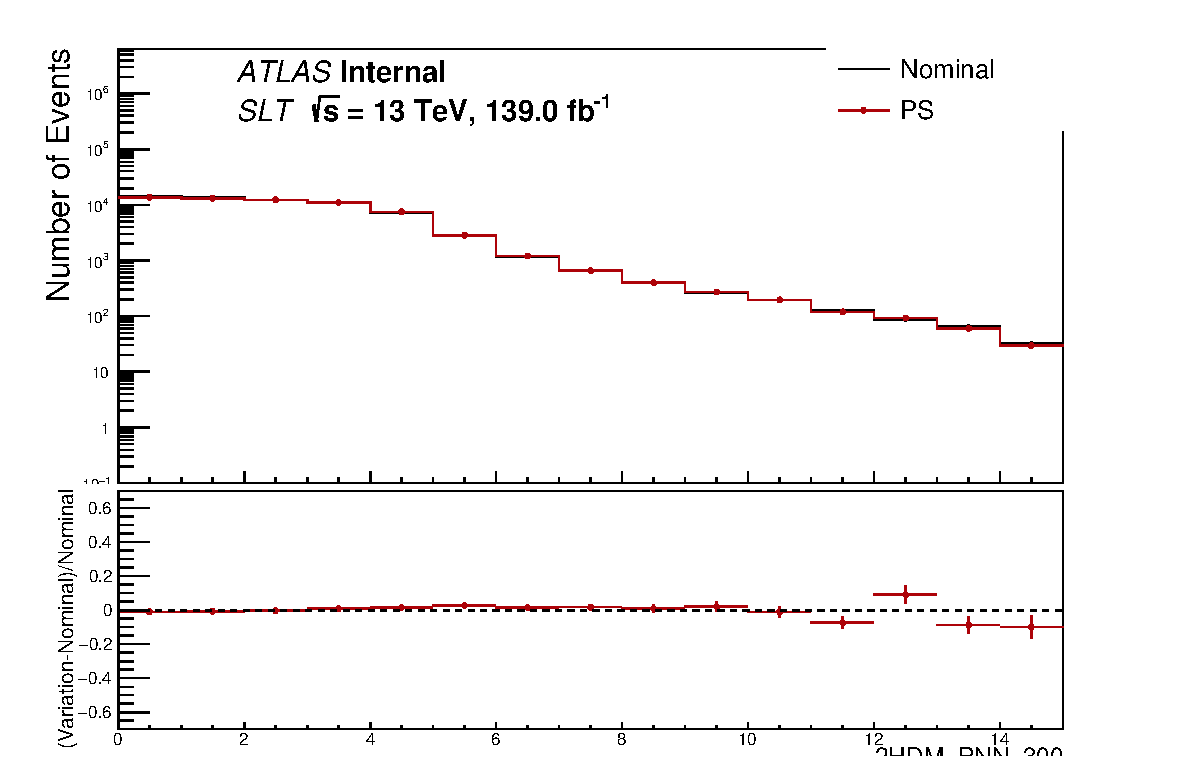
\includegraphics[width=.41\textwidth]{figures/lephad_modelling_systs/SLT/PS/limit_binning_2HDM_PNN_300_Norm}
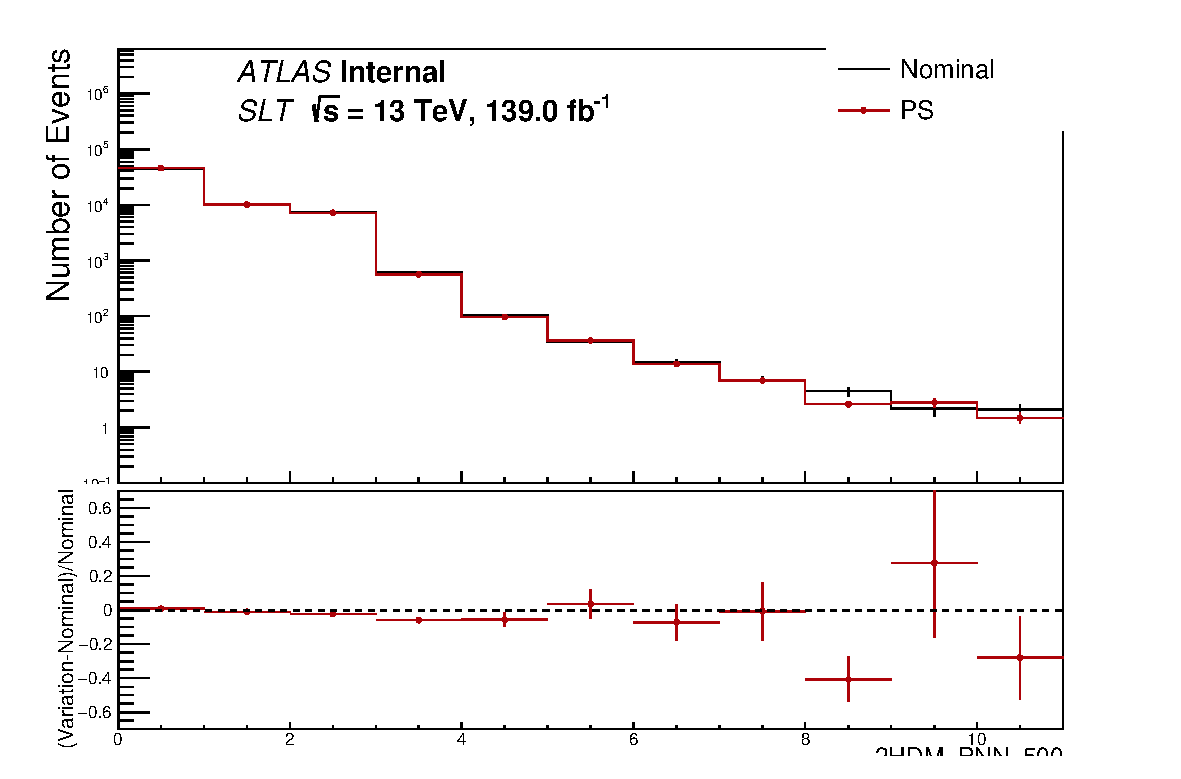
\includegraphics[width=.41\textwidth]{figures/lephad_modelling_systs/SLT/PS/limit_binning_2HDM_PNN_500_Norm}\\
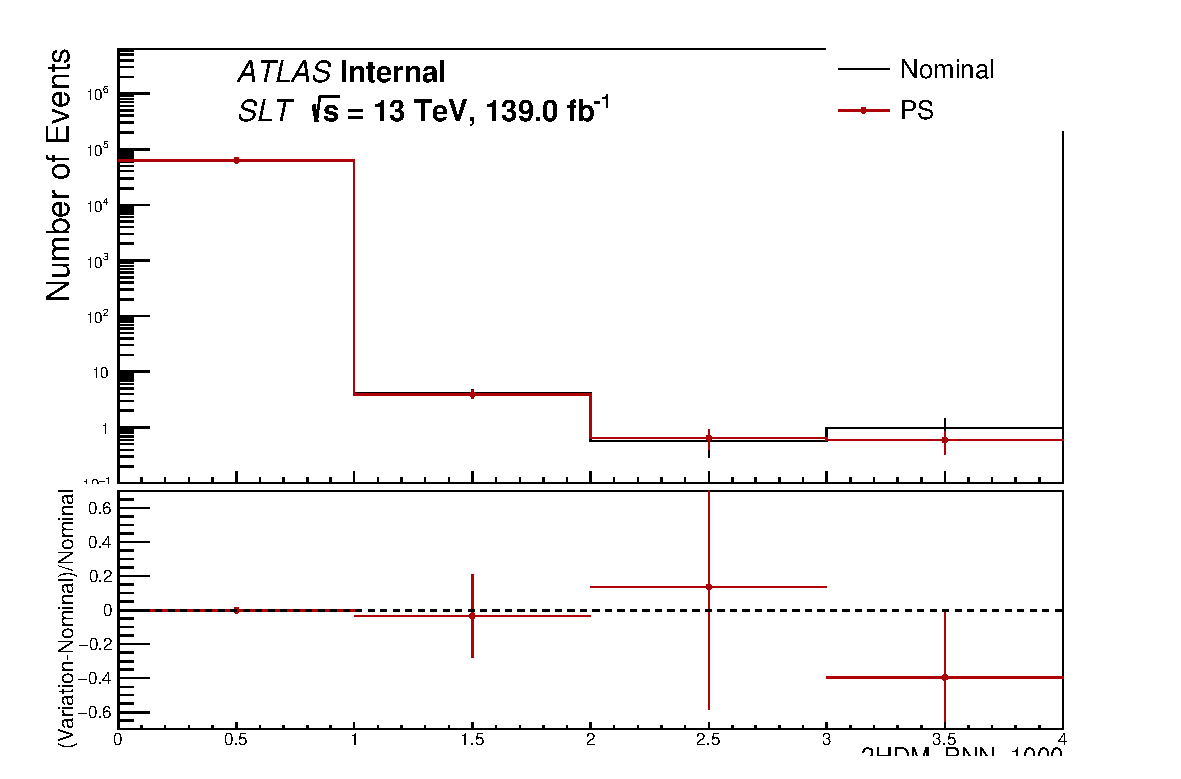
\includegraphics[width=.41\textwidth]{figures/lephad_modelling_systs/SLT/PS/limit_binning_2HDM_PNN_1000_Norm}
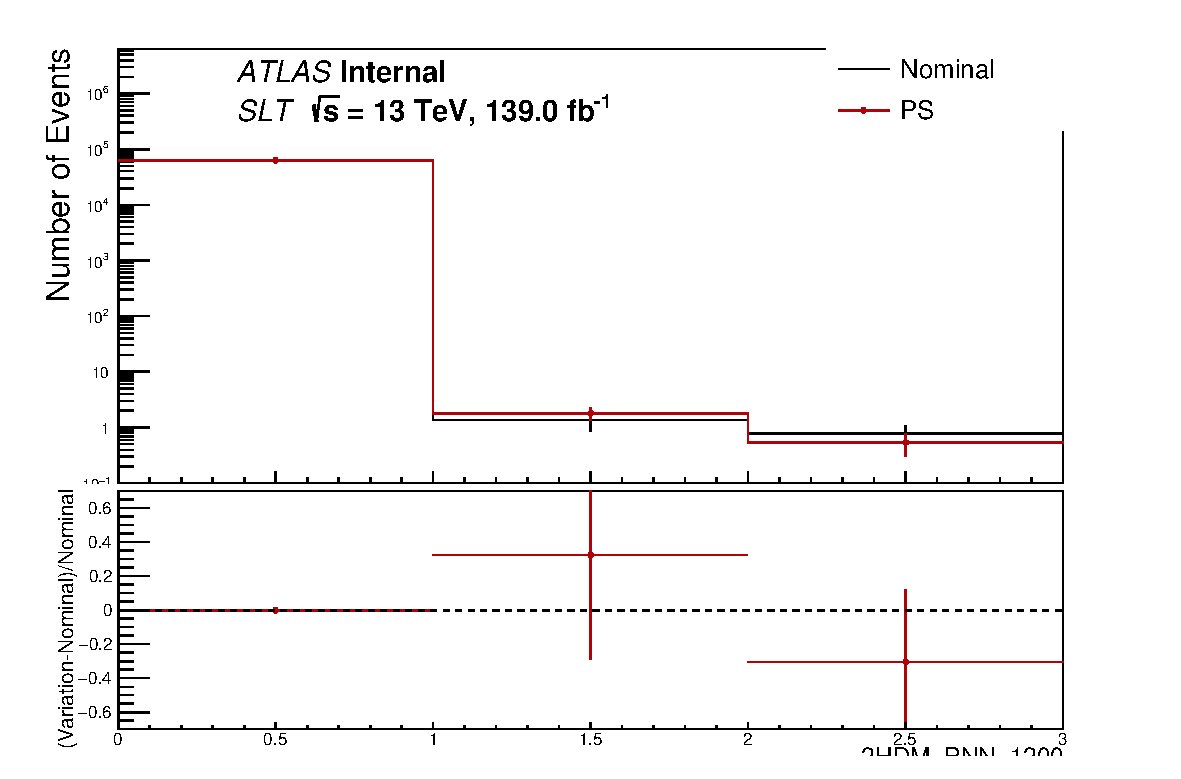
\includegraphics[width=.41\textwidth]{figures/lephad_modelling_systs/SLT/PS/limit_binning_2HDM_PNN_1200_Norm}
\caption{Shape-only ratio of the PS variation to the nominal in PNN score of various resonant mass.}
\label{fig:ttbarsyst_lephad_PS_SLT_PNN}
\end{figure}


\begin{figure}
\centering
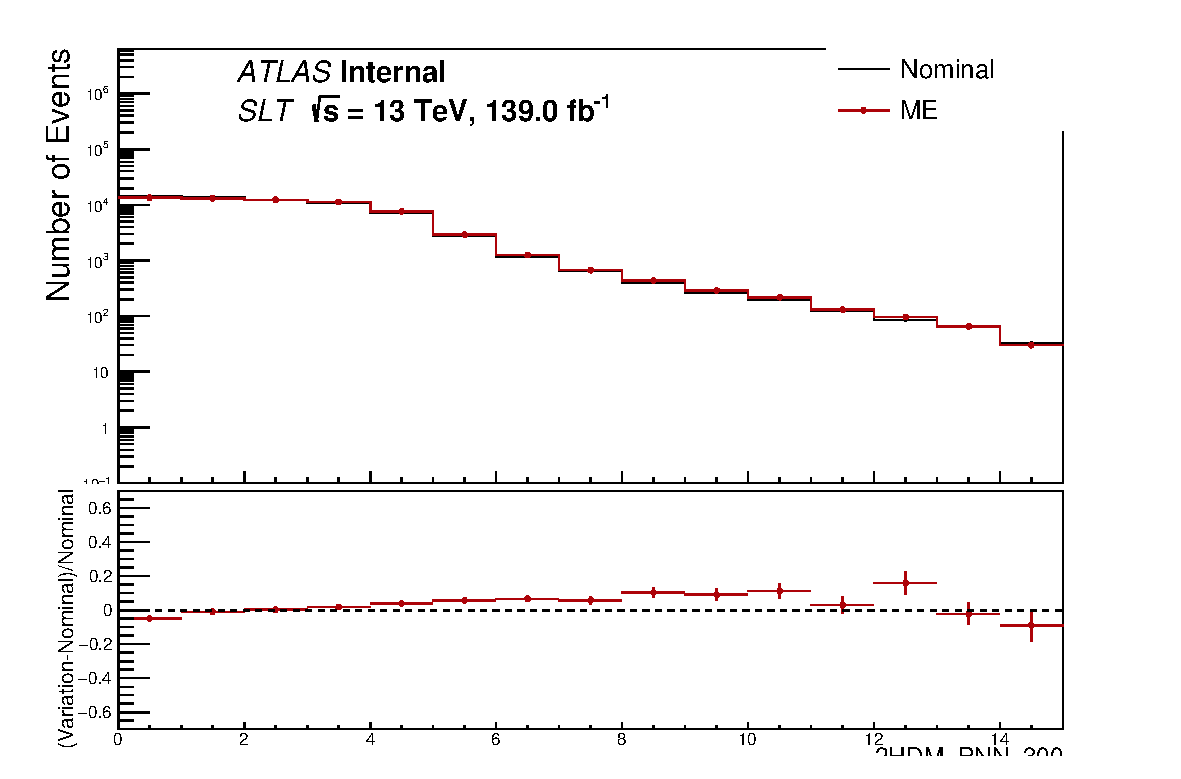
\includegraphics[width=.41\textwidth]{figures/lephad_modelling_systs/SLT/ME/limit_binning_2HDM_PNN_300_Norm}
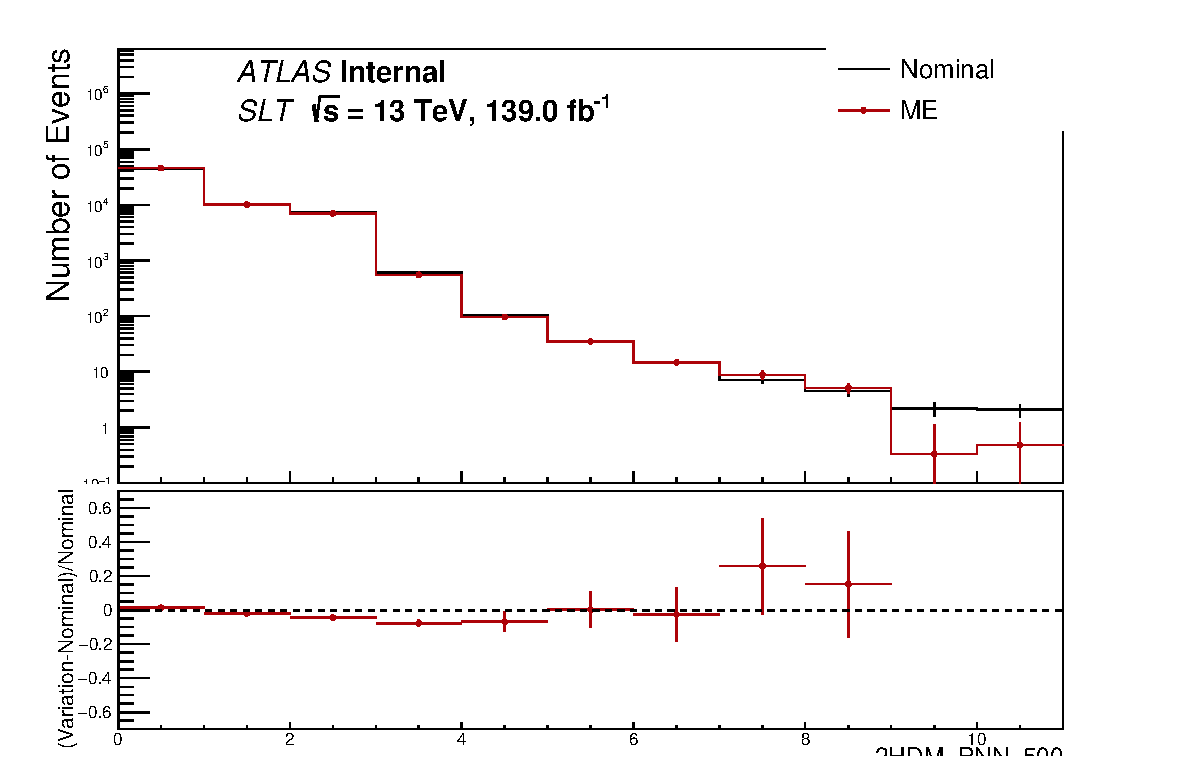
\includegraphics[width=.41\textwidth]{figures/lephad_modelling_systs/SLT/ME/limit_binning_2HDM_PNN_500_Norm}\\
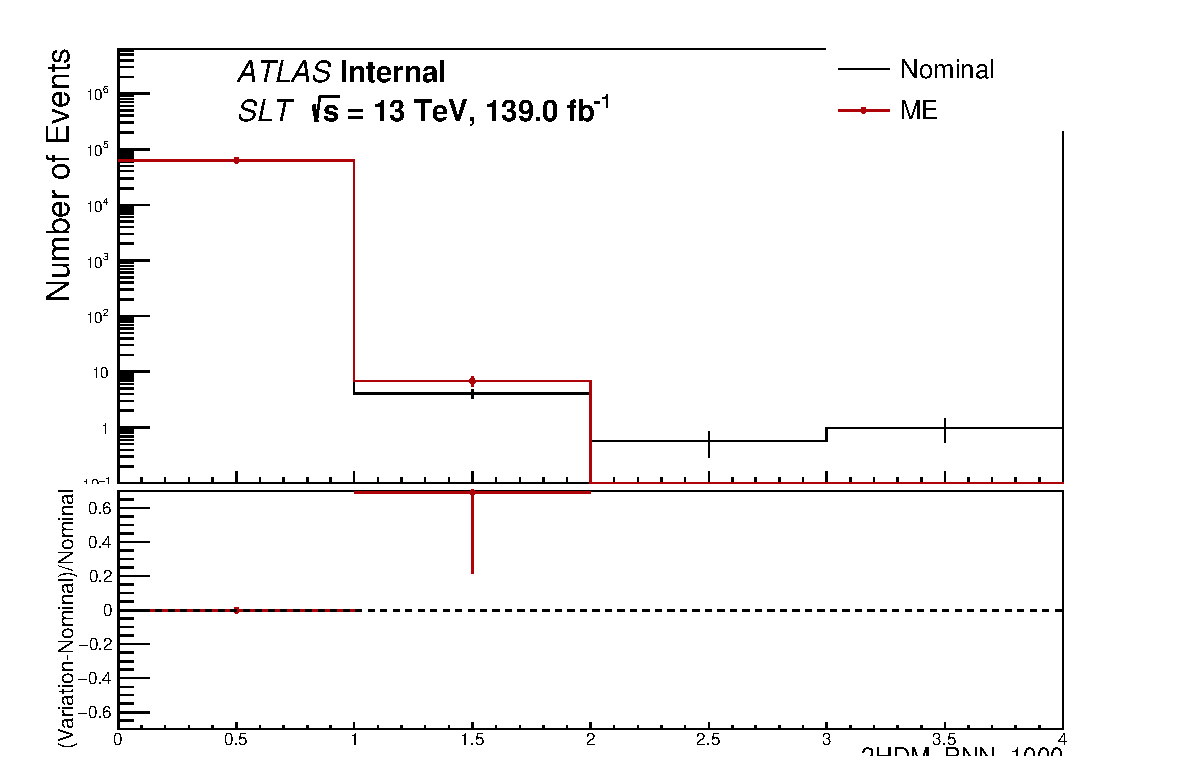
\includegraphics[width=.41\textwidth]{figures/lephad_modelling_systs/SLT/ME/limit_binning_2HDM_PNN_1000_Norm}
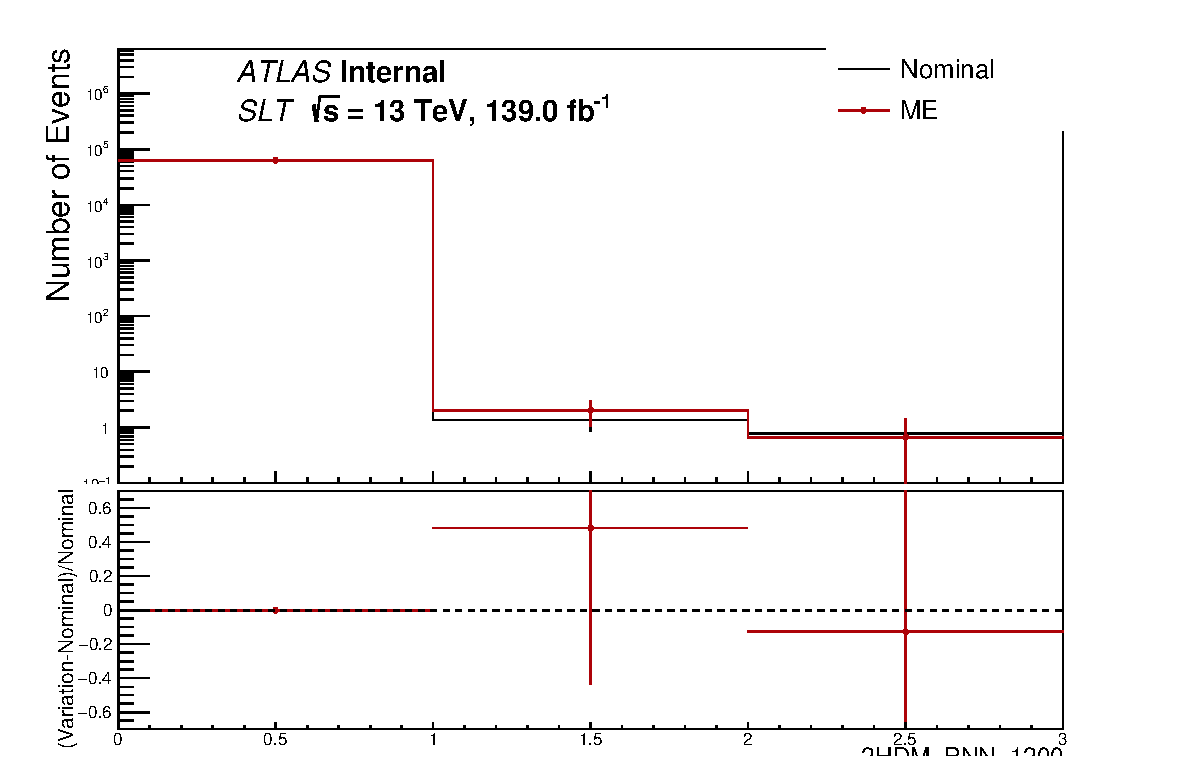
\includegraphics[width=.41\textwidth]{figures/lephad_modelling_systs/SLT/ME/limit_binning_2HDM_PNN_1200_Norm}
\caption{Shape-only ratio of the ME variation to the nominal in PNN score of various resonant mass.}
\label{fig:ttbarsyst_lephad_ME_SLT_PNN}
\end{figure}


\begin{figure}[htbp]
  \centering
  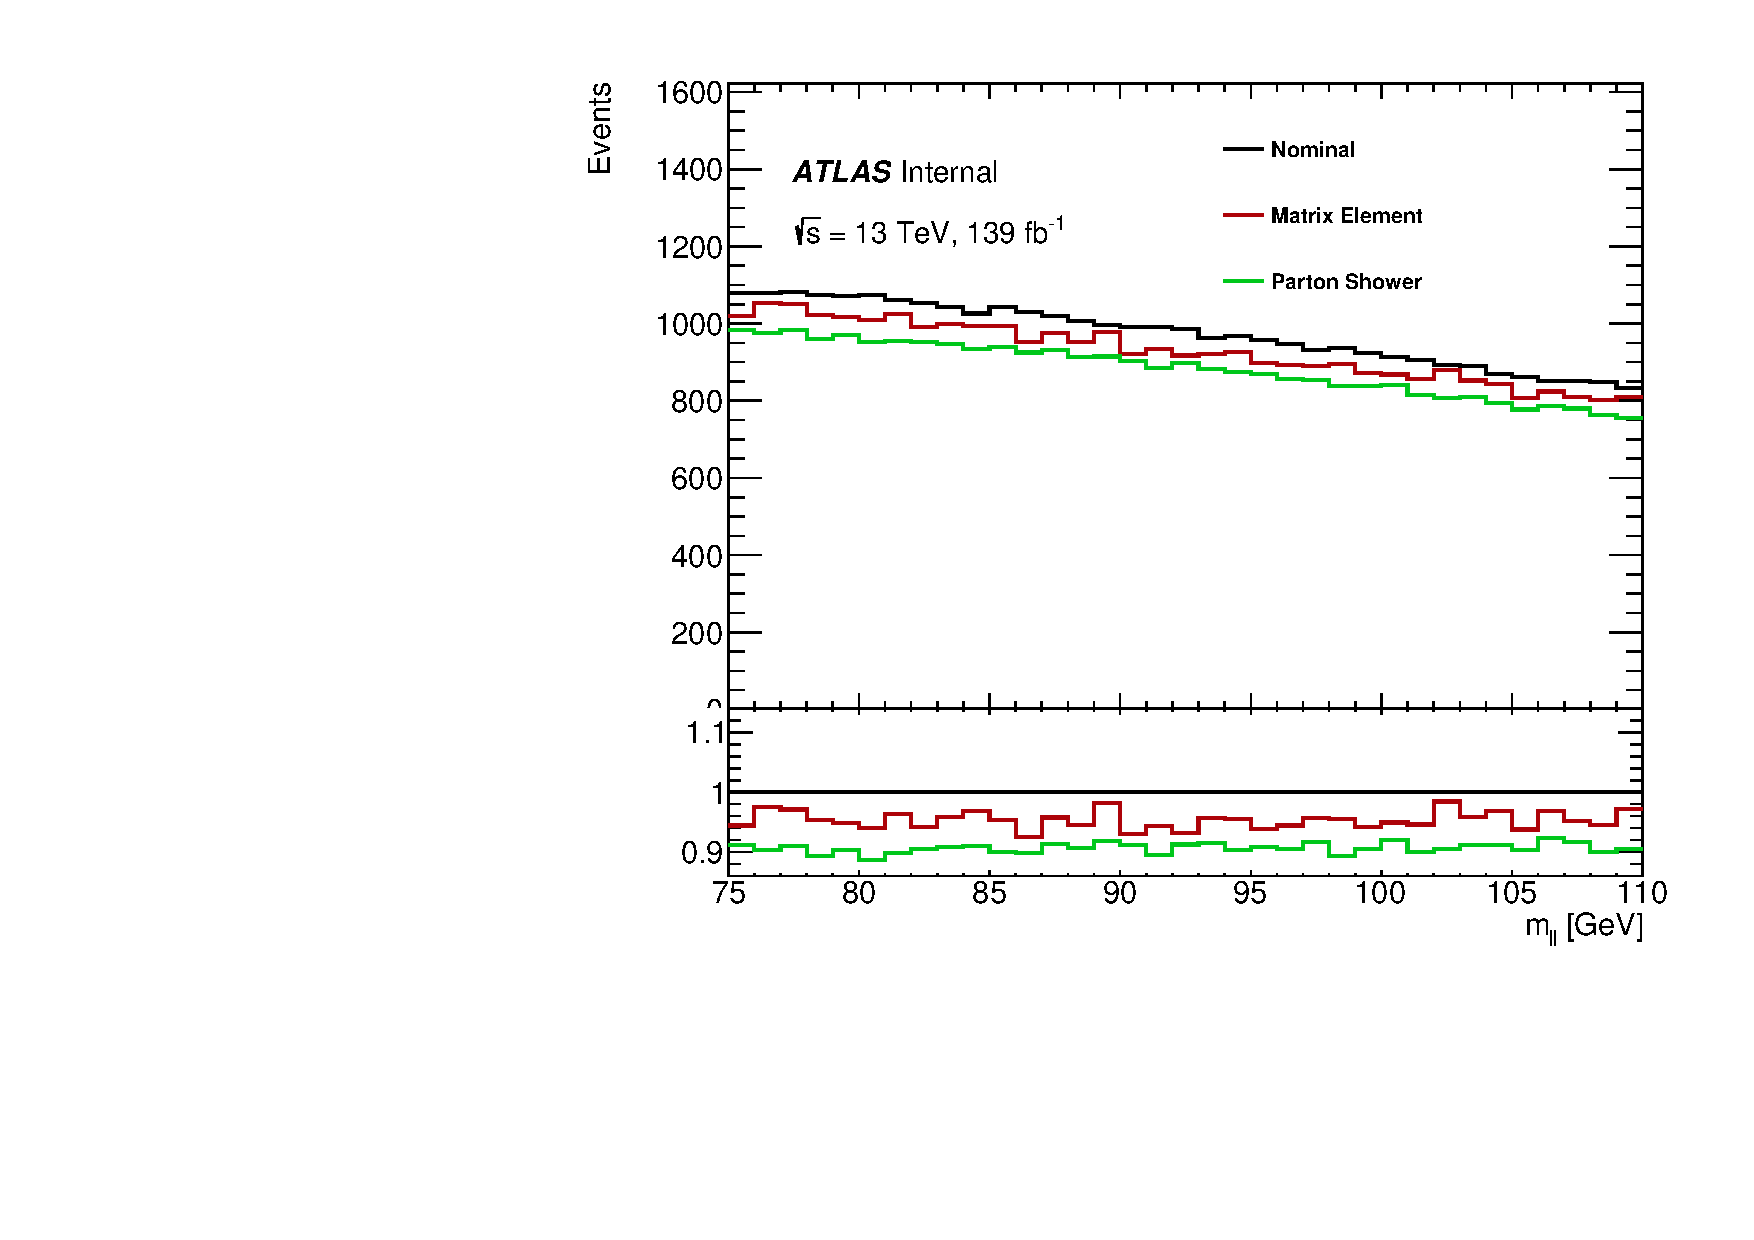
\includegraphics[width=0.45\textwidth]{figures/appendix/ZHFSys/ttbar_alter.pdf}
  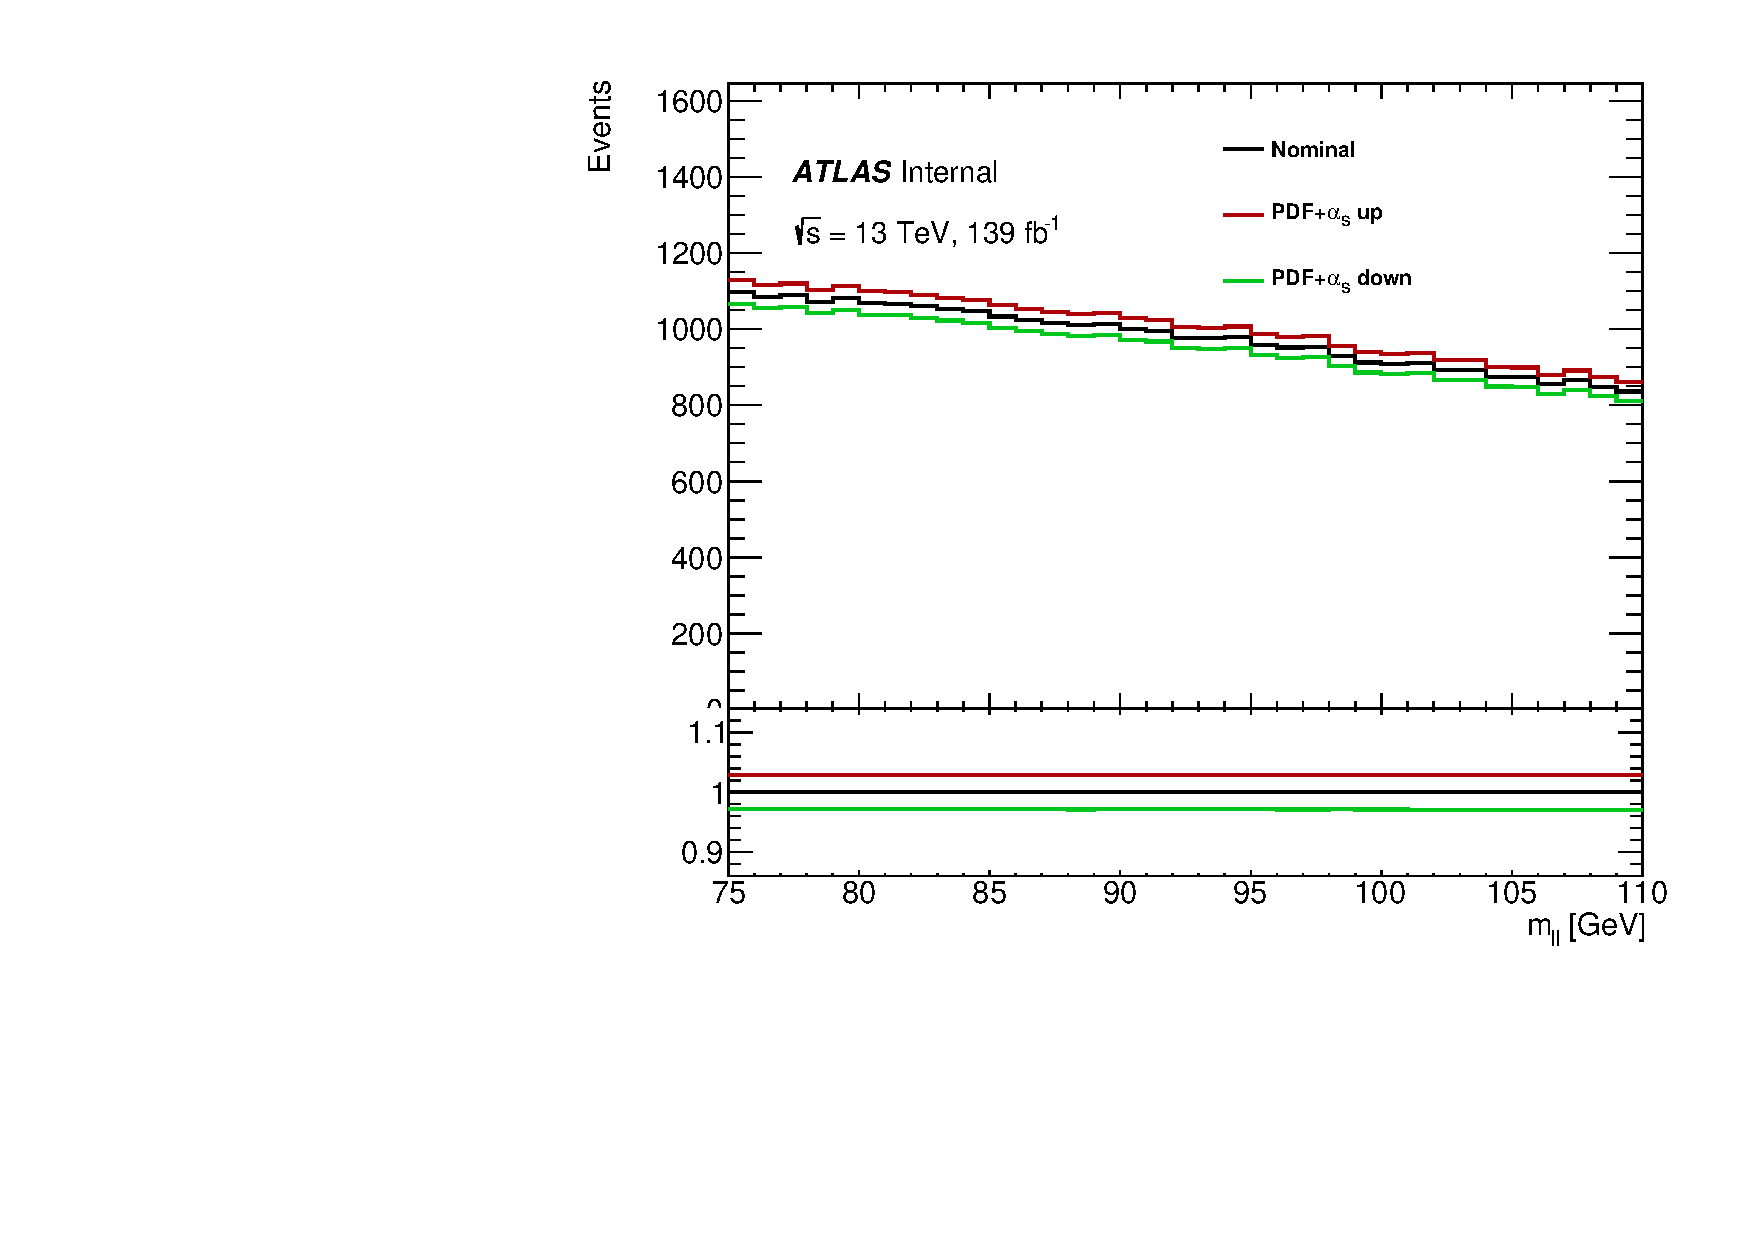
\includegraphics[width=0.45\textwidth]{figures/appendix/ZHFSys/ttbar_pdf.pdf} \\
  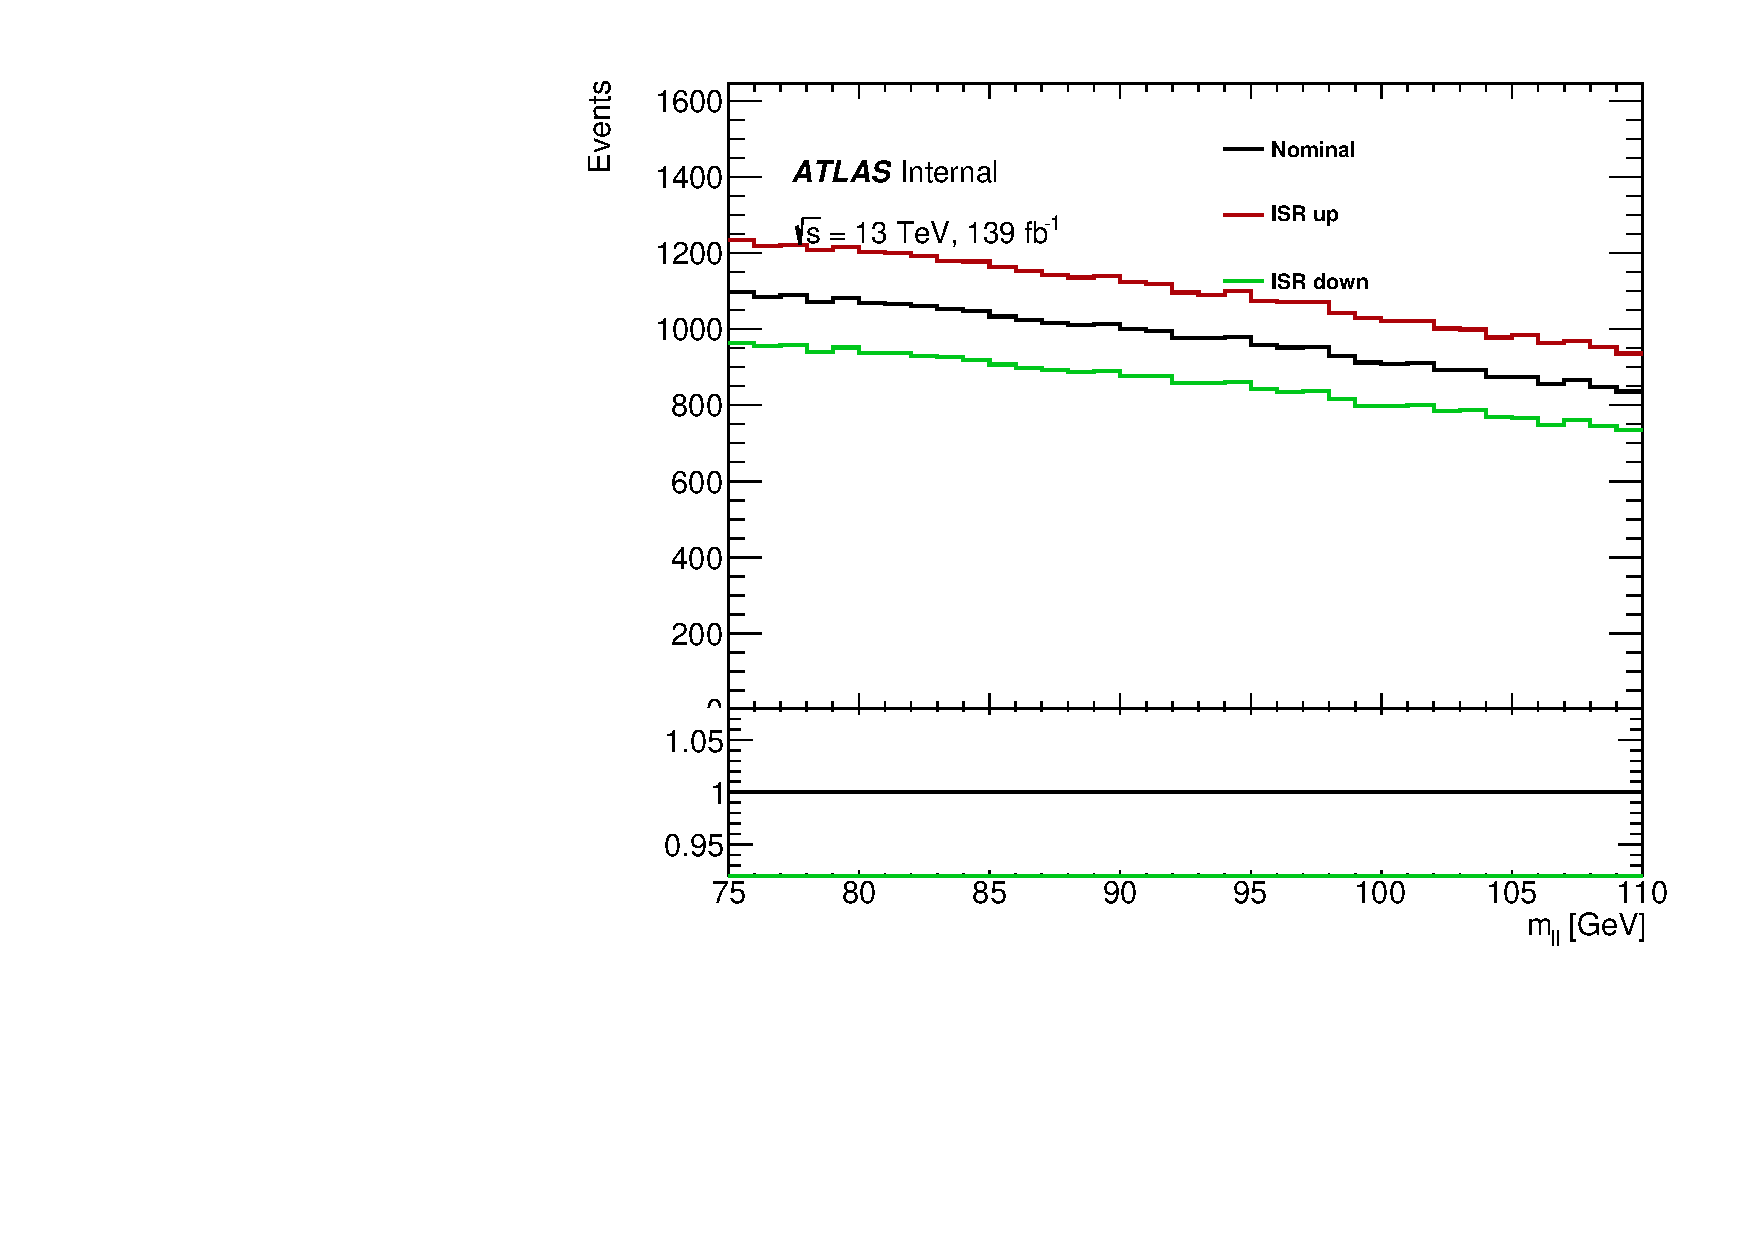
\includegraphics[width=0.45\textwidth]{figures/appendix/ZHFSys/ttbar_ISR.pdf}
  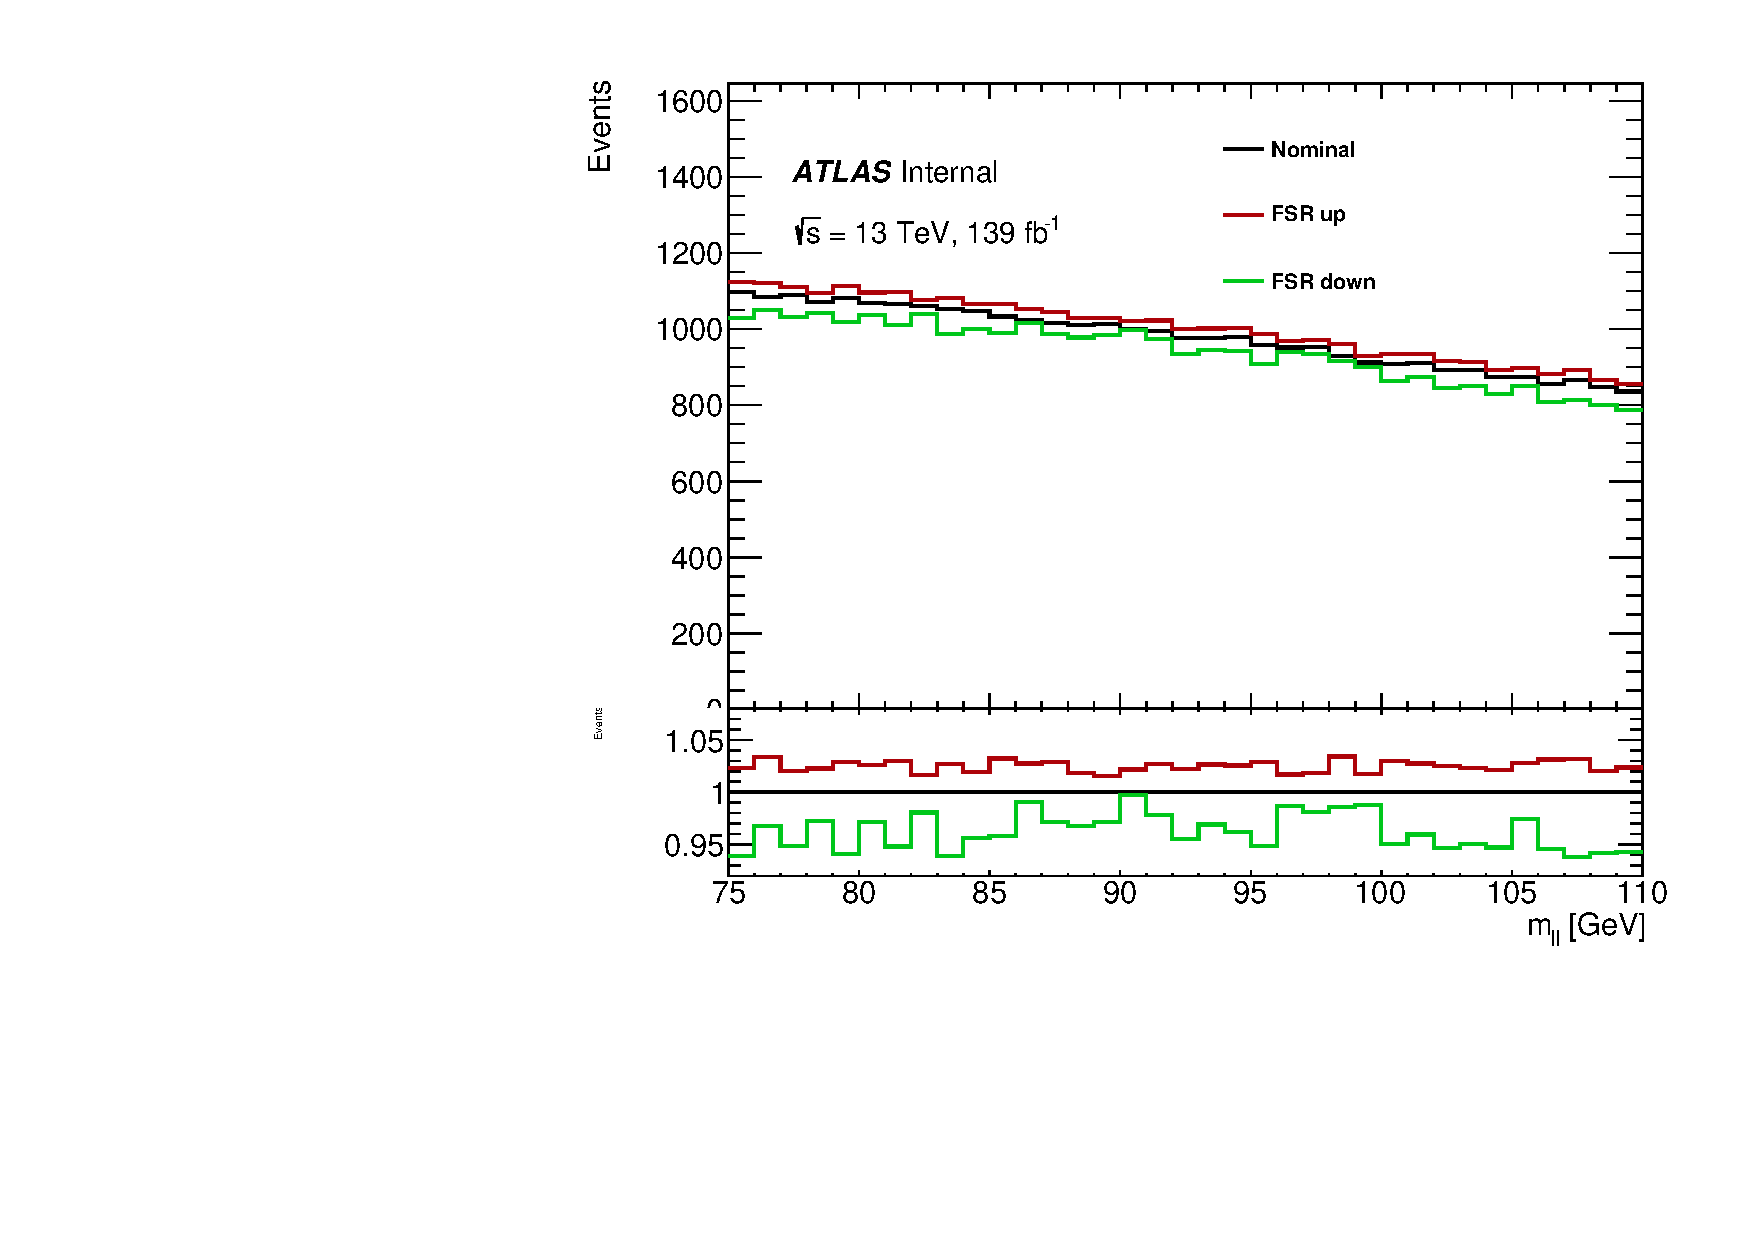
\includegraphics[width=0.45\textwidth]{figures/appendix/ZHFSys/ttbar_FSR.pdf} \\
  \caption{$m_{ll}$ spectra comparisons for nominal and systematics from matrix element and parton
  shower (top left), PDF+$\alpha_{S}$ (top right), ISR (bottom left) and FSR (bottom right).
  Images reproced from analysis internal notes. 
  }
  \label{fig:append:ZHFttbar}
\end{figure}



 



\begin{figure}
   \centering
   \subfloat[]
      {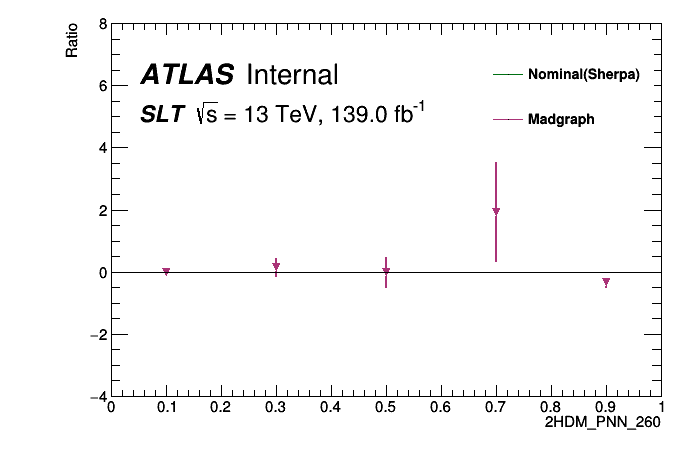
\includegraphics[width=.41\textwidth]{figures/lephad_modelling_systs/SLT/ZHF_Madgraph_SLT/Ratio_2HDM_PNN_260_Norm.png}} \quad
   \subfloat[]
      {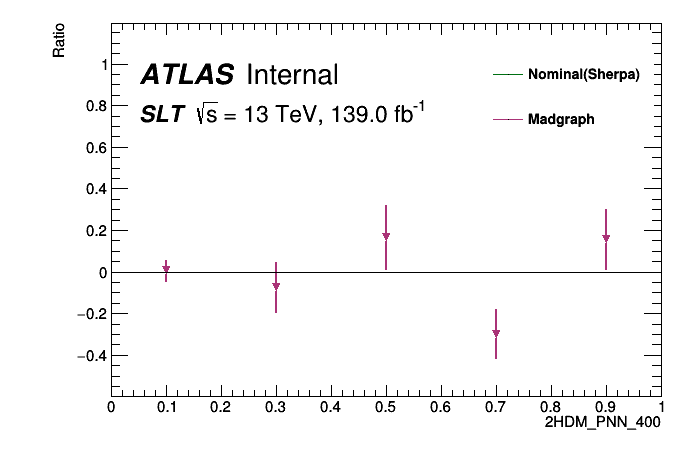
\includegraphics[width=.41\textwidth]{figures/lephad_modelling_systs/SLT/ZHF_Madgraph_SLT/Ratio_2HDM_PNN_400_Norm.png}} \quad
   \subfloat[]
      {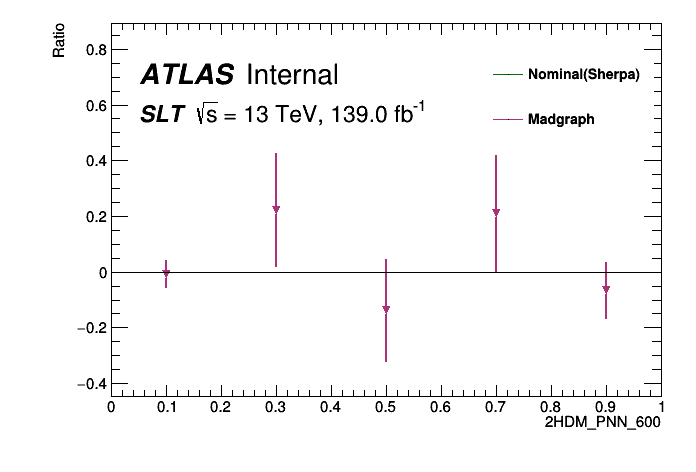
\includegraphics[width=.41\textwidth]{figures/lephad_modelling_systs/SLT/ZHF_Madgraph_SLT/Ratio_2HDM_PNN_600_Norm.png}} \quad
   \subfloat[]
      {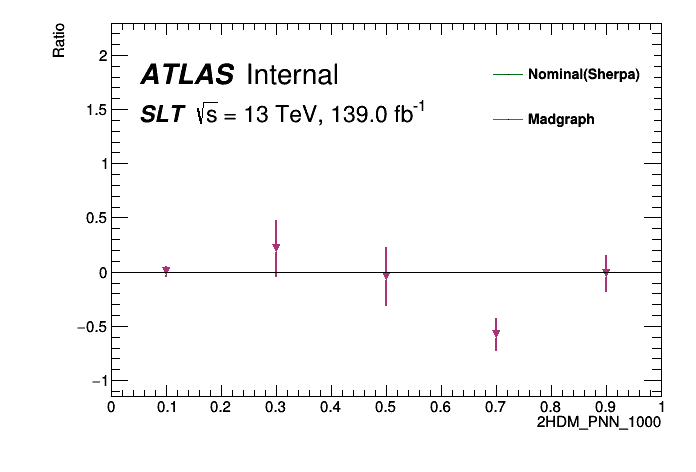
\includegraphics[width=.41\textwidth]{figures/lephad_modelling_systs/SLT/ZHF_Madgraph_SLT/Ratio_2HDM_PNN_1000_Norm.png}} \quad
   \caption{SLT channel: comparision of the nominal Sherpa sample verse the variation Madgraph in the PNN score distribtuion.}
   \label{fig:lephad_ZHF_Madgraph_SLT_PNN}
   \end{figure}
   
\begin{figure}
   \centering
   \subfloat[]
      {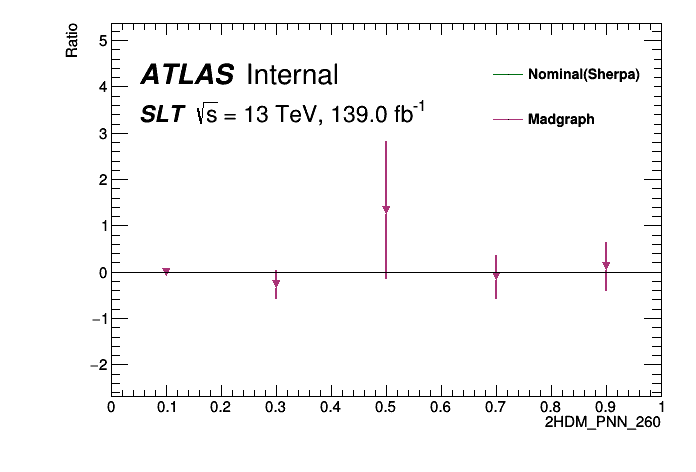
\includegraphics[width=.41\textwidth]{figures/lephad_modelling_systs/LTT/ZHF_Madgraph_LTT/Ratio_2HDM_PNN_260_Norm.png}} \quad
   \subfloat[]
      {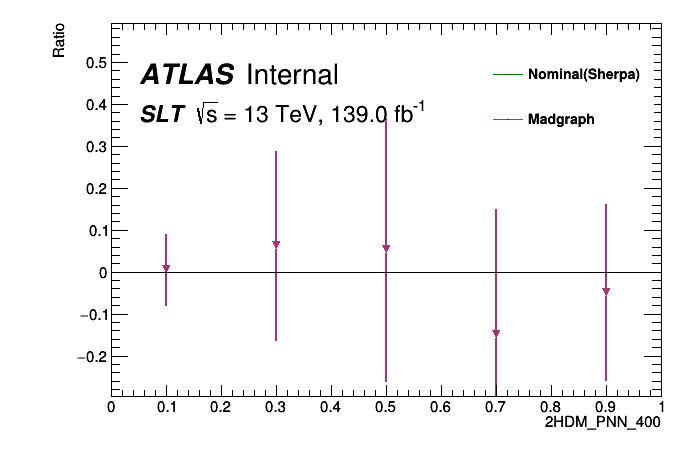
\includegraphics[width=.41\textwidth]{figures/lephad_modelling_systs/LTT/ZHF_Madgraph_LTT/Ratio_2HDM_PNN_400_Norm.png}} \quad
   \subfloat[]
      {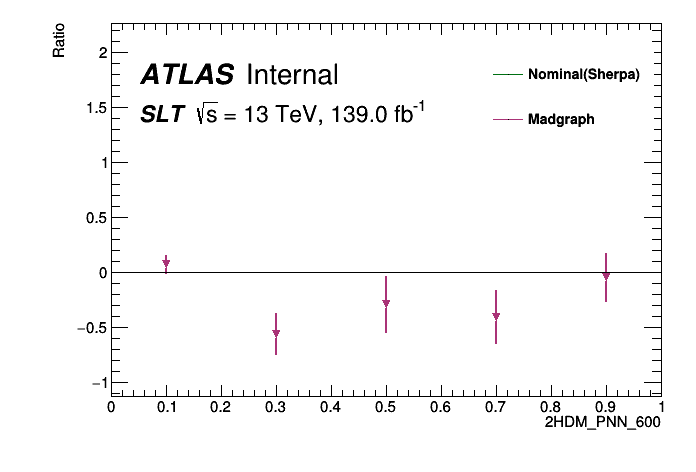
\includegraphics[width=.41\textwidth]{figures/lephad_modelling_systs/LTT/ZHF_Madgraph_LTT/Ratio_2HDM_PNN_600_Norm.png}} \quad
   \subfloat[]
      {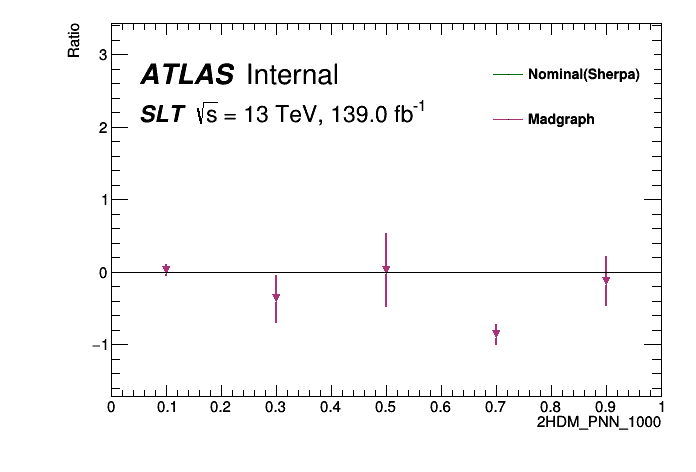
\includegraphics[width=.41\textwidth]{figures/lephad_modelling_systs/LTT/ZHF_Madgraph_LTT/Ratio_2HDM_PNN_1000_Norm.png}} \quad
   \caption{LTT channel: comparision of the nominal Sherpa sample verse the variation Madgraph in the PNN score distribtuion.}
   \label{fig:lephad_ZHF_Madgraph_LTT_PNN}
   \end{figure}
      





\begin{figure}
\centering
\subfloat[]
   {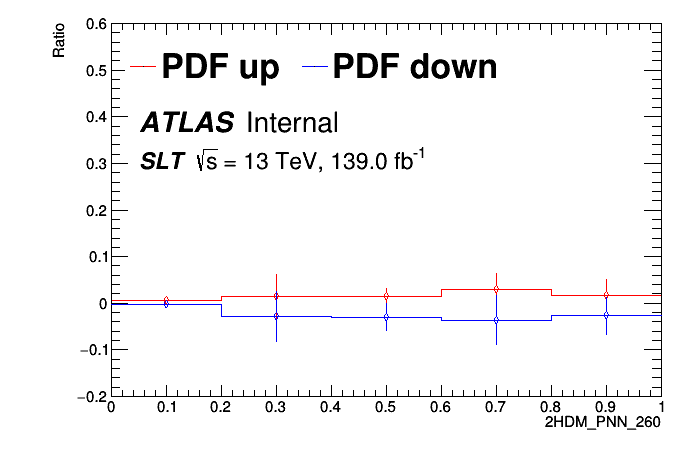
\includegraphics[width=.41\textwidth]{figures/lephad_modelling_systs/SLT/ZHF_PDF/Ratio_2HDM_PNN_260_Norm.png}} \quad
\subfloat[]
   {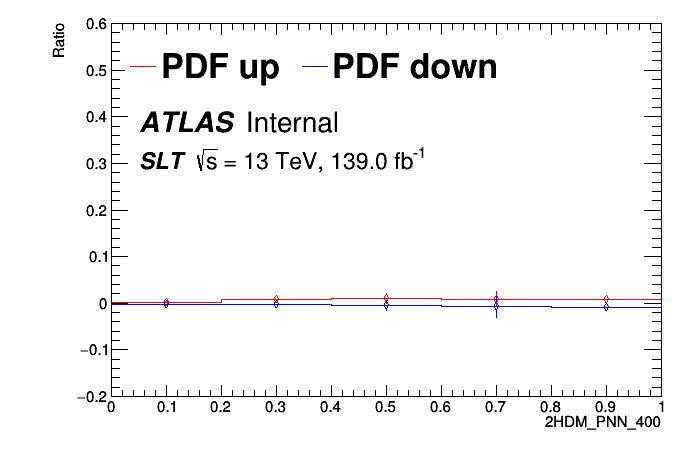
\includegraphics[width=.41\textwidth]{figures/lephad_modelling_systs/SLT/ZHF_PDF/Ratio_2HDM_PNN_400_Norm.png}} \quad
\subfloat[]
   {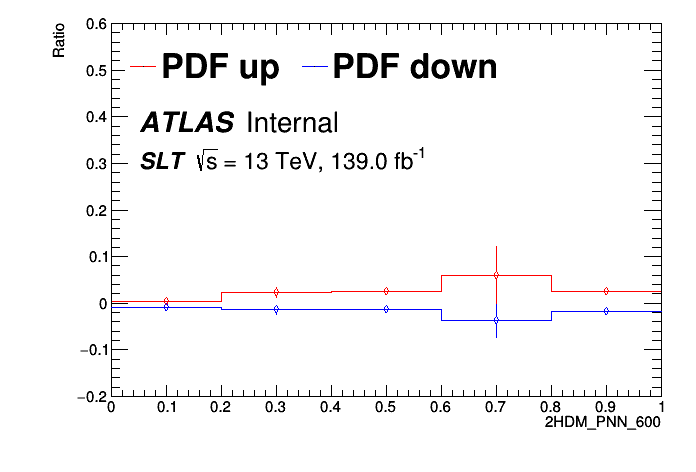
\includegraphics[width=.41\textwidth]{figures/lephad_modelling_systs/SLT/ZHF_PDF/Ratio_2HDM_PNN_600_Norm.png}} \quad
\subfloat[]
   {\includegraphics[width=.41\textwidth]{figures/lephad_modelling_systs/SLT/ZHF_PDF/Ratio_2HDM_PNN_800_Norm.png}} \quad
\caption{SLT channel: Z+HF intra-PDF variation in PNN score of various resonant mass.}
\label{fig:lephad_ZHF_PDF_SLT_PNN}
\end{figure}




\begin{figure}
\centering
\subfloat[]
   {\includegraphics[width=.41\textwidth]{figures/lephad_modelling_systs/LTT/ZHF_PDF/Ratio_2HDM_PNN_260_Norm.png}} \quad
\subfloat[]
   {\includegraphics[width=.41\textwidth]{figures/lephad_modelling_systs/LTT/ZHF_PDF/Ratio_2HDM_PNN_400_Norm.png}} \quad
\subfloat[]
   {\includegraphics[width=.41\textwidth]{figures/lephad_modelling_systs/LTT/ZHF_PDF/Ratio_2HDM_PNN_600_Norm.png}} \quad
\subfloat[]
   {\includegraphics[width=.41\textwidth]{figures/lephad_modelling_systs/LTT/ZHF_PDF/Ratio_2HDM_PNN_800_Norm.png}} \quad
\caption{LTT channel: Z+HF intra-PDF variation in the PNN score of various resonant masses.}
\label{fig:lephad_ZHF_PDF_LTT_PNN}
\end{figure}





\begin{figure}
\centering
\subfloat[]
   {\includegraphics[width=.41\textwidth]{figures/lephad_modelling_systs/SLT/ZHF_nnlo/Ratio_2HDM_PNN_260_Norm.png}} \quad
\subfloat[]
   {\includegraphics[width=.41\textwidth]{figures/lephad_modelling_systs/SLT/ZHF_nnlo/Ratio_2HDM_PNN_400_Norm.png}} \quad
\subfloat[]
   {\includegraphics[width=.41\textwidth]{figures/lephad_modelling_systs/SLT/ZHF_nnlo/Ratio_2HDM_PNN_600_Norm.png}} \quad
\subfloat[]
   {\includegraphics[width=.41\textwidth]{figures/lephad_modelling_systs/SLT/ZHF_nnlo/Ratio_2HDM_PNN_800_Norm.png}} \quad
\caption{SLT channel: Z+HF inter-PDF variations and $\alpha_s$ variations in PNN score of various resonant mass.}
\label{fig:lephad_ZHF_nnlo_SLT_PNN}
\end{figure}




\begin{figure}
\centering
\subfloat[]
   {\includegraphics[width=.41\textwidth]{figures/lephad_modelling_systs/LTT/ZHF_nnlo/Ratio_2HDM_PNN_260_Norm.png}} \quad
\subfloat[]
   {\includegraphics[width=.41\textwidth]{figures/lephad_modelling_systs/LTT/ZHF_nnlo/Ratio_2HDM_PNN_400_Norm.png}} \quad
\subfloat[]
   {\includegraphics[width=.41\textwidth]{figures/lephad_modelling_systs/LTT/ZHF_nnlo/Ratio_2HDM_PNN_600_Norm.png}} \quad
\subfloat[]
   {\includegraphics[width=.41\textwidth]{figures/lephad_modelling_systs/LTT/ZHF_nnlo/Ratio_2HDM_PNN_800_Norm.png}} \quad
\caption{LTT channel: Z+HF inter-PDF variations and $\alpha_s$ variations in the PNN score of various resonant masses.}
\label{fig:lephad_ZHF_nnlo_LTT_PNN}
\end{figure}




\begin{figure}
\centering
\subfloat[]
   {\includegraphics[width=.41\textwidth]{figures/lephad_modelling_systs/SLT/ZHF_ckkw/Ratio_2HDM_PNN_260_Norm.png}} \quad
\subfloat[]
   {\includegraphics[width=.41\textwidth]{figures/lephad_modelling_systs/SLT/ZHF_ckkw/Ratio_2HDM_PNN_400_Norm.png}} \quad
\subfloat[]
   {\includegraphics[width=.41\textwidth]{figures/lephad_modelling_systs/SLT/ZHF_ckkw/Ratio_2HDM_PNN_600_Norm.png}} \quad
\subfloat[]
   {\includegraphics[width=.41\textwidth]{figures/lephad_modelling_systs/SLT/ZHF_ckkw/Ratio_2HDM_PNN_800_Norm.png}} \quad
\caption{SLT channel: Z+HF ckkw and qsf variations in PNN score of various resonant mass.}
\label{fig:lephad_ZHF_ckkw_SLT_PNN}
\end{figure}




\begin{figure}
\centering
\subfloat[]
   {\includegraphics[width=.41\textwidth]{figures/lephad_modelling_systs/LTT/ZHF_ckkw/Ratio_2HDM_PNN_260_Norm.png}} \quad
\subfloat[]
   {\includegraphics[width=.41\textwidth]{figures/lephad_modelling_systs/LTT/ZHF_ckkw/Ratio_2HDM_PNN_400_Norm.png}} \quad
\subfloat[]
   {\includegraphics[width=.41\textwidth]{figures/lephad_modelling_systs/LTT/ZHF_ckkw/Ratio_2HDM_PNN_600_Norm.png}} \quad
\subfloat[]
   {\includegraphics[width=.41\textwidth]{figures/lephad_modelling_systs/LTT/ZHF_ckkw/Ratio_2HDM_PNN_800_Norm.png}} \quad
\caption{LTT channel:Z+HF ckkw and qsf variations in the PNN score of various resonant masses.}
\label{fig:lephad_ZHF_ckkw_LTT_PNN}
\end{figure}



\begin{figure}
\centering
\includegraphics[width=0.32\textwidth]{figures/appendix/ZHFSys/Zmm_scale.pdf} 
\includegraphics[width=0.32\textwidth]{figures/appendix/ZHFSys/Zmm_ckkw.pdf}
\includegraphics[width=0.32\textwidth]{figures/appendix/ZHFSys/Zmm_qsf.pdf} \\
\includegraphics[width=0.32\textwidth]{figures/appendix/ZHFSys/Zee_scale.pdf} 
\includegraphics[width=0.32\textwidth]{figures/appendix/ZHFSys/Zee_ckkw.pdf}
\includegraphics[width=0.32\textwidth]{figures/appendix/ZHFSys/Zee_qsf.pdf} \\ 
\includegraphics[width=0.32\textwidth]{figures/appendix/ZHFSys/Zee_pdf.pdf}
\includegraphics[width=0.32\textwidth]{figures/appendix/ZHFSys/Zee_alt_pdf.pdf}
\includegraphics[width=0.3\textwidth]{figures/appendix/ZHFSys/Zhf_MGvsSherpa.pdf} 
\caption{Top row: the $m_{ll}$ spectra comparisons for nominal
 and systematics from scale variations
(left), ckkw (middle) and qsf (right) on Z($\rightarrow \mu \mu$) 
+ HF (first row) and $Z(\rightarrow \ell\ell)$+HF (second row) processes.
Bottom row: the $m_{ll}$ spectra comparisons for nominal and 
systematics from PDF+$\alpha_{S}$ (left)
and alternative PDF (middle) variations for $Z(\rightarrow ee)$+HF 
process and on the right for the nominal Sherpa generator and alternative MadGraph 
generator for $Z(\rightarrow \ell\ell)$+HF process.
Images reproduced from analysis internal notes. 
}
\label{fig:append:ZHF}
\end{figure}



\begin{figure}
\centering
\includegraphics[width=.45\textwidth]{figures/lephad_modelling_systs/SLT/singletop/Herwig/Hist_and_ratio_SM_NN_Norm}         
\includegraphics[width=.45\textwidth]{figures/lephad_modelling_systs/SLT/singletop/Herwig/Hist_and_ratio_2HDM_PNN_260_Norm}   \\
\includegraphics[width=.45\textwidth]{figures/lephad_modelling_systs/SLT/singletop/Herwig/Hist_and_ratio_2HDM_PNN_400_Norm}    
\includegraphics[width=.45\textwidth]{figures/lephad_modelling_systs/SLT/singletop/Herwig/Hist_and_ratio_2HDM_PNN_600_Norm}   \\
\includegraphics[width=.45\textwidth]{figures/lephad_modelling_systs/SLT/singletop/Herwig/Hist_and_ratio_2HDM_PNN_800_Norm}   

\caption{SLT channel: shape-only PS uncertainty in the NN and PNN score of various resonant masses.}
\label{fig:singletopsyst_lephad_herwig_PNN_SLT}
\end{figure}

\begin{figure}
\centering
\includegraphics[width=.45\textwidth]{figures/lephad_modelling_systs/LTT/singletop/Herwig/Hist_and_ratio_SM_NN_Norm}    
\includegraphics[width=.45\textwidth]{figures/lephad_modelling_systs/LTT/singletop/Herwig/Hist_and_ratio_2HDM_PNN_260_Norm}   \\
\includegraphics[width=.45\textwidth]{figures/lephad_modelling_systs/LTT/singletop/Herwig/Hist_and_ratio_2HDM_PNN_400_Norm}    
\includegraphics[width=.45\textwidth]{figures/lephad_modelling_systs/LTT/singletop/Herwig/Hist_and_ratio_2HDM_PNN_600_Norm}   \\
\includegraphics[width=.45\textwidth]{figures/lephad_modelling_systs/LTT/singletop/Herwig/Hist_and_ratio_2HDM_PNN_800_Norm}    
\caption{LTT channel: shape-only PS uncertainty in the NN and PNN score of various resonant masses.}
\label{fig:singletopsyst_lephad_herwig_PNN_LTT}
\end{figure}


\begin{figure}
\centering
\includegraphics[width=.45\textwidth]{figures/lephad_modelling_systs/SLT/singletop/aMC/Hist_and_ratio_SM_NN_Norm}         
\includegraphics[width=.45\textwidth]{figures/lephad_modelling_systs/SLT/singletop/aMC/Hist_and_ratio_2HDM_PNN_260_Norm}   \\
\includegraphics[width=.45\textwidth]{figures/lephad_modelling_systs/SLT/singletop/aMC/Hist_and_ratio_2HDM_PNN_400_Norm}    
\includegraphics[width=.45\textwidth]{figures/lephad_modelling_systs/SLT/singletop/aMC/Hist_and_ratio_2HDM_PNN_600_Norm}   \\
\includegraphics[width=.45\textwidth]{figures/lephad_modelling_systs/SLT/singletop/aMC/Hist_and_ratio_2HDM_PNN_800_Norm}   

\caption{SLT channel: shape-only ME uncertainty in the NN and PNN score of various resonant masses.}
\label{fig:singletopsyst_lephad_aMC_PNN_SLT}
\end{figure}

\begin{figure}
   \centering
\includegraphics[width=.45\textwidth]{figures/lephad_modelling_systs/LTT/singletop/aMC/Hist_and_ratio_SM_NN_Norm}    
\includegraphics[width=.45\textwidth]{figures/lephad_modelling_systs/LTT/singletop/aMC/Hist_and_ratio_2HDM_PNN_260_Norm}   \\
\includegraphics[width=.45\textwidth]{figures/lephad_modelling_systs/LTT/singletop/aMC/Hist_and_ratio_2HDM_PNN_400_Norm}    
\includegraphics[width=.45\textwidth]{figures/lephad_modelling_systs/LTT/singletop/aMC/Hist_and_ratio_2HDM_PNN_600_Norm}   \\
\includegraphics[width=.45\textwidth]{figures/lephad_modelling_systs/LTT/singletop/aMC/Hist_and_ratio_2HDM_PNN_800_Norm}    
\caption{LTT channel: shape-only ME uncertainty in the NN and PNN score of various resonant masses.}
\label{fig:singletopsyst_lephad_aMC_PNN_LTT}
\end{figure}



\begin{figure}
\centering       
\includegraphics[width=.45\textwidth]{figures/lephad_modelling_systs/SLT/singletop/interference/Hist_and_ratio_2HDM_PNN_260_Norm}   
\includegraphics[width=.45\textwidth]{figures/lephad_modelling_systs/SLT/singletop/interference/Hist_and_ratio_2HDM_PNN_400_Norm}   \\ 
\includegraphics[width=.45\textwidth]{figures/lephad_modelling_systs/SLT/singletop/interference/Hist_and_ratio_2HDM_PNN_600_Norm}   
\includegraphics[width=.45\textwidth]{figures/lephad_modelling_systs/SLT/singletop/interference/Hist_and_ratio_2HDM_PNN_800_Norm}   \\

\caption{SLT channel: shape-only interference uncertainty in the PNN score of various resonant masses.}
\label{fig:singletopsyst_lephad_interference_PNN_SLT}
\end{figure}

\begin{figure}
      \centering
\includegraphics[width=.45\textwidth]{figures/lephad_modelling_systs/LTT/singletop/interference/Hist_and_ratio_2HDM_PNN_260_Norm}   
\includegraphics[width=.45\textwidth]{figures/lephad_modelling_systs/LTT/singletop/interference/Hist_and_ratio_2HDM_PNN_400_Norm}   \\ 
\includegraphics[width=.45\textwidth]{figures/lephad_modelling_systs/LTT/singletop/interference/Hist_and_ratio_2HDM_PNN_600_Norm}   
\includegraphics[width=.45\textwidth]{figures/lephad_modelling_systs/LTT/singletop/interference/Hist_and_ratio_2HDM_PNN_800_Norm}  \\  
\caption{LTT channel: shape-only interference uncertainty in the PNN score of various resonant masses.}
\label{fig:singletopsyst_lephad_interference_PNN_LTT}
\end{figure}



The resonant signal PS uncertainties are parametrised by linear functions. 
The function used in the SLT SR is:
\begin{itemize}
\item Down variation = 1.82 - 0.95 * PNN Score.
\item Up variation = 0.18 + 0.95 * PNN Score;
\end{itemize}
The function used in the LTT SR is:
\begin{itemize}
\item Down variation = 1.84 - 1.01 * PNN Score;
\item Up variation = 0.16 + 1.01 * PNN Score.
\end{itemize}
\begin{figure}
\centering
\includegraphics[width=.49\textwidth]{figures/systs/LepHad_Signal_SLT_500_psSysts_PNN_Fit_Logy.pdf}
\includegraphics[width=.49\textwidth]{figures/systs/LepHad_Signal_SLT_1000_psSysts_PNN_Fit_Logy.pdf}
\caption{Comparison of the SLT signal PNN distributions obtained from 
the nominal (black) and alternative (blue) signal samples for the PS variations for 
the  $m_X= 500$ GeV (left) and the $m_X=1000$ GeV (right) mass points. 
A linear fit to the ratio of the two distributions is performed 
and shown in the lower panel of the figures (red line). 
The variations obtained from the linear function obtained from the $m_X= 500$ 
GeV fit are also shown in the figures (green and magenta).
Image reproduced from analysis internal notes.}
\label{fig:LepHadSLTSignalSysts}
\end{figure}

\begin{figure}
\centering
\includegraphics[width=.49\textwidth]{figures/systs/LepHad_Signal_LTT_500_psSysts_PNN_Fit_Logy.pdf}
\includegraphics[width=.49\textwidth]{figures/systs/LepHad_Signal_LTT_1000_psSysts_PNN_Fit_Logy.pdf}
\caption{Comparison of the LTT signal PNN distributions 
obtained from the nominal (black) and alternative (blue) 
signal samples for the PS variations for the  $m_X= 500$ GeV (left) 
and the $m_X=1000$ GeV (right) mass points. 
A linear fit to the ratio of the two distributions is performed and 
shown in the lower panel of the figures (red line). 
The variations obtained from the linear function obtained from the $m_X= 500$ 
GeV fit are also shown in the figures (green and magenta).
Image reproduced from analysis internal notes.}
\label{fig:LepHadLTTSignalSysts}
\end{figure}



%%% lephad plots to be replaced with the proper binning. Also only SLT shown here. %%%

\begin{figure}[tbh!]
   \subfloat[$\kappa_\lambda=0$]{
       \includegraphics[width=0.45\linewidth]{DiHiggs/plots/kl_scan/bbtautauSubchannels/lephad_VBF_rw_kl0_NN_SLT.png}
   }
   \subfloat[$\kappa_\lambda=2$]{
       \includegraphics[width=0.45\linewidth]{DiHiggs/plots/kl_scan/bbtautauSubchannels/lephad_VBF_rw_kl2_NN_SLT.png}
   }\
   \caption{Closure plots for the linear combination of VBF samples for 
   two different bases in the $\tau_{\text{lep}}\tau_{\text{had}}$ channel. 
   NN score distributions for the MC $\kappa_\lambda = 0, 2$ samples (orange) and the 
   reweighted ones (blue) are shown together with their ratio. 
   The largest difference between the two distributions is of 2.2\% (SLT) and 
   stems from the linear combination of VBF samples $(\kappa_\lambda = 1, 10, 0)$ to  $\kappa_\lambda=2$.
   Figure reproduced from analysis internal notes.}
   \label{fig:bbtautau_lephad_VBFclosure}
\end{figure}


















The data driven fakes estimated with $t\bar{t}$ variation 
samples are shown in Fig.\ref{fig:ttbarsyst_lephad_Fakes_SLT_PNN} 
for the SLT channel and Fig.\ref{fig:ttbarsyst_lephad_Fakes_LTT_PNN} for the LTT channel. 
In Fig.\ref{fig:ttbarsyst_lephad_Fakes_SLT_PNN_ratio} 
and Fig.\ref{fig:ttbarsyst_lephad_Fakes_LTT_PNN_ratio}, the y-axis shows the rate 
of differences between the fakes estimated with $t\bar{t}$ variation samples and 
the nominal $t\bar{t}$ sample, to the nominal $t\bar{t}$ sample. 
The nominal $t\bar{t}$ sample is fast simulation sample and it's compared 
to the fast simulation variation $t\bar{t}$ samples. 
These variation samples includes the uncertainties from the matrix elements, 
parton shower selection and the initial state radiation. 
The final state radiation radiation on the other hand 
is estimated with the full simulation $t\bar{t}$ sample internal weights, 
as shown in Fig.\ref{fig:ttbarsyst_lephad_Fakes_SLT_PNN_fullsim} 
for the SLT channel and Fig.\ref{fig:ttbarsyst_lephad_Fakes_LTT_PNN_fullsim} 
for the LTT channel. Similarly the ratios are 
shwon in Fig.\ref{fig:ttbarsyst_lephad_Fakes_SLT_PNN_ratio_fullsim} 
for the SLT channel and Fig.\ref{fig:ttbarsyst_lephad_Fakes_LTT_PNN_ratio_fullsim} 
for the LTT channel. 







\begin{figure}[htbp] 
\centering
\subfloat[]
   {\includegraphics[width=.41\textwidth]{figures/lephad_modelling_systs/SLT/data_fakes/purehist2HDM_PNN_260}} \quad
\subfloat[]
   {\includegraphics[width=.41\textwidth]{figures/lephad_modelling_systs/SLT/data_fakes/purehist2HDM_PNN_400}} \quad
\subfloat[]
   {\includegraphics[width=.41\textwidth]{figures/lephad_modelling_systs/SLT/data_fakes/purehist2HDM_PNN_600}} \quad
\subfloat[]
   {\includegraphics[width=.41\textwidth]{figures/lephad_modelling_systs/SLT/data_fakes/purehist2HDM_PNN_800}} \quad
\caption{SLT channel: data driven fakes estimated with the nominal $t\bar{t}$ sample and the variation $t\bar{t}$ sample.}
\label{fig:ttbarsyst_lephad_Fakes_SLT_PNN}
\end{figure}




\begin{figure}[htbp]
\centering
\subfloat[]
   {\includegraphics[width=.41\textwidth]{figures/lephad_modelling_systs/LTT/data_fakes/purehist2HDM_PNN_260}} \quad
\subfloat[]
   {\includegraphics[width=.41\textwidth]{figures/lephad_modelling_systs/LTT/data_fakes/purehist2HDM_PNN_400}} \quad
\subfloat[]
   {\includegraphics[width=.41\textwidth]{figures/lephad_modelling_systs/LTT/data_fakes/purehist2HDM_PNN_600}} \quad
\subfloat[]
   {\includegraphics[width=.41\textwidth]{figures/lephad_modelling_systs/LTT/data_fakes/purehist2HDM_PNN_800}} \quad
\caption{LTT channel: data driven fakes estimated with the nominal $t\bar{t}$ sample and the variation $t\bar{t}$ sample.}
\label{fig:ttbarsyst_lephad_Fakes_LTT_PNN}
\end{figure}





\begin{figure}[htbp]
\centering
\subfloat[]
   {\includegraphics[width=.41\textwidth]{figures/lephad_modelling_systs/SLT/data_fakes/2HDM_PNN_260}} \quad
\subfloat[]
   {\includegraphics[width=.41\textwidth]{figures/lephad_modelling_systs/SLT/data_fakes/2HDM_PNN_400}} \quad
\subfloat[]
   {\includegraphics[width=.41\textwidth]{figures/lephad_modelling_systs/SLT/data_fakes/2HDM_PNN_600}} \quad
\subfloat[]
   {\includegraphics[width=.41\textwidth]{figures/lephad_modelling_systs/SLT/data_fakes/2HDM_PNN_800}} \quad
\caption{SLT channel: data driven fakes estimated with the nominal $t\bar{t}$ sample and the variation $t\bar{t}$ sample.}
\label{fig:ttbarsyst_lephad_Fakes_SLT_PNN_ratio}
\end{figure}




\begin{figure}[htbp]
\centering
\subfloat[]
   {\includegraphics[width=.41\textwidth]{figures/lephad_modelling_systs/LTT/data_fakes/2HDM_PNN_260}} \quad
\subfloat[]
   {\includegraphics[width=.41\textwidth]{figures/lephad_modelling_systs/LTT/data_fakes/2HDM_PNN_400}} \quad
\subfloat[]
   {\includegraphics[width=.41\textwidth]{figures/lephad_modelling_systs/LTT/data_fakes/2HDM_PNN_600}} \quad
\subfloat[]
   {\includegraphics[width=.41\textwidth]{figures/lephad_modelling_systs/LTT/data_fakes/2HDM_PNN_800}} \quad
\caption{LTT channel: data driven fakes estimated with the nominal $t\bar{t}$ sample and the variation $t\bar{t}$ sample.}
\label{fig:ttbarsyst_lephad_Fakes_LTT_PNN_ratio}
\end{figure}





\begin{figure}[htbp]
\centering
\subfloat[]
   {\includegraphics[width=.41\textwidth]{figures/lephad_modelling_systs/SLT/FSR_down/purehist2HDM_PNN_260}} \quad
\subfloat[]
   {\includegraphics[width=.41\textwidth]{figures/lephad_modelling_systs/SLT/FSR_down/purehist2HDM_PNN_400}} \quad
\subfloat[]
   {\includegraphics[width=.41\textwidth]{figures/lephad_modelling_systs/SLT/FSR_down/purehist2HDM_PNN_600}} \quad
\subfloat[]
   {\includegraphics[width=.41\textwidth]{figures/lephad_modelling_systs/SLT/FSR_down/purehist2HDM_PNN_800}} \quad
\caption{SLT channel: data driven fakes estimated with the nominal $t\bar{t}$ sample and the variation $t\bar{t}$ sample.}
\label{fig:ttbarsyst_lephad_Fakes_SLT_PNN_fullsim}
\end{figure}




\begin{figure}[htbp]
\centering
\subfloat[]
   {\includegraphics[width=.41\textwidth]{figures/lephad_modelling_systs/LTT/FSR_down/purehist2HDM_PNN_260}} \quad
\subfloat[]
   {\includegraphics[width=.41\textwidth]{figures/lephad_modelling_systs/LTT/FSR_down/purehist2HDM_PNN_400}} \quad
\subfloat[]
   {\includegraphics[width=.41\textwidth]{figures/lephad_modelling_systs/LTT/FSR_down/purehist2HDM_PNN_600}} \quad
\subfloat[]
   {\includegraphics[width=.41\textwidth]{figures/lephad_modelling_systs/LTT/FSR_down/purehist2HDM_PNN_800}} \quad
\caption{LTT channel: data driven fakes estimated with the nominal $t\bar{t}$ sample and the variation $t\bar{t}$ sample.}
\label{fig:ttbarsyst_lephad_Fakes_LTT_PNN_fullsim}
\end{figure}





\begin{figure}[htbp]
\centering
\subfloat[]
   {\includegraphics[width=.41\textwidth]{figures/lephad_modelling_systs/SLT/FSR_down/2HDM_PNN_260}} \quad
\subfloat[]
   {\includegraphics[width=.41\textwidth]{figures/lephad_modelling_systs/SLT/FSR_down/2HDM_PNN_400}} \quad
\subfloat[]
   {\includegraphics[width=.41\textwidth]{figures/lephad_modelling_systs/SLT/FSR_down/2HDM_PNN_600}} \quad
\subfloat[]
   {\includegraphics[width=.41\textwidth]{figures/lephad_modelling_systs/SLT/FSR_down/2HDM_PNN_800}} \quad
\caption{SLT channel: data driven fakes estimated with the nominal $t\bar{t}$ sample and the variation $t\bar{t}$ sample.}
\label{fig:ttbarsyst_lephad_Fakes_SLT_PNN_ratio_fullsim}
\end{figure}




\begin{figure}[htbp]
\centering
\subfloat[]
   {\includegraphics[width=.41\textwidth]{figures/lephad_modelling_systs/LTT/FSR_down/2HDM_PNN_260}} \quad
\subfloat[]
   {\includegraphics[width=.41\textwidth]{figures/lephad_modelling_systs/LTT/FSR_down/2HDM_PNN_400}} \quad
\subfloat[]
   {\includegraphics[width=.41\textwidth]{figures/lephad_modelling_systs/LTT/FSR_down/2HDM_PNN_600}} \quad
\subfloat[]
   {\includegraphics[width=.41\textwidth]{figures/lephad_modelling_systs/LTT/FSR_down/2HDM_PNN_800}} \quad
\caption{LTT channel: data driven fakes estimated with the nominal $t\bar{t}$ sample and the variation $t\bar{t}$ sample.}
\label{fig:ttbarsyst_lephad_Fakes_LTT_PNN_ratio_fullsim}
\end{figure}


\section{Additional material for results}

\label{sec:appendix:result}
\begin{figure}
   \centering
   \includegraphics[width=.32\textwidth]{figures/results/HH/LepHad/Region_BMin0_incJet1_dist300_J2_D2HDMPNN_T1_SpcTauLH_Y2015_LTT0_L1_GlobalFit_conditionnal_mu0log.pdf}
   \includegraphics[width=.32\textwidth]{figures/results/HH/LepHad/Region_BMin0_incJet1_dist500_J2_D2HDMPNN_T1_SpcTauLH_Y2015_LTT0_L1_GlobalFit_conditionnal_mu0log.pdf}
   \includegraphics[width=.32\textwidth]{figures/results/HH/LepHad/Region_BMin0_incJet1_dist1000_J2_D2HDMPNN_T1_SpcTauLH_Y2015_LTT0_L1_GlobalFit_conditionnal_mu0log.pdf} \\
   \includegraphics[width=.32\textwidth]{figures/results/HH/LepHad/Region_BMin0_incJet1_dist1600_J2_D2HDMPNN_T1_SpcTauLH_Y2015_LTT0_L1_GlobalFit_conditionnal_mu0log.pdf}
   \includegraphics[width=.32\textwidth]{figures/results/HH/LepHad/Region_BMin0_incJet1_distNN_J2_DSM_T1_SpcTauLH_Y2015_LTT0_L1_GlobalFit_conditionnal_mu0log.pdf} \\
   \includegraphics[width=.32\textwidth]{figures/results/HH/LepHad/Region_BMin0_incJet1_dist300_J2_D2HDMPNN_T1_SpcTauLH_Y2015_LTT1_L1_GlobalFit_conditionnal_mu0log.pdf}
   \includegraphics[width=.32\textwidth]{figures/results/HH/LepHad/Region_BMin0_incJet1_dist500_J2_D2HDMPNN_T1_SpcTauLH_Y2015_LTT1_L1_GlobalFit_conditionnal_mu0log.pdf}
   \includegraphics[width=.32\textwidth]{figures/results/HH/LepHad/Region_BMin0_incJet1_dist1000_J2_D2HDMPNN_T1_SpcTauLH_Y2015_LTT1_L1_GlobalFit_conditionnal_mu0log.pdf} \\
   \includegraphics[width=.32\textwidth]{figures/results/HH/LepHad/Region_BMin0_incJet1_dist1600_J2_D2HDMPNN_T1_SpcTauLH_Y2015_LTT1_L1_GlobalFit_conditionnal_mu0log.pdf}
   \includegraphics[width=.32\textwidth]{figures/results/HH/LepHad/Region_BMin0_incJet1_distNN_J2_DSM_T1_SpcTauLH_Y2015_LTT1_L1_GlobalFit_conditionnal_mu0log.pdf}
   \caption{Post-fit PNN score distributions for the $300, 500, 1000, 1600$ GeV mass points 
   and non-resonant NN in the di-Higgs $bb\lephad$ SLT (top two rows) and LTT (bottom two rows) 1 b-tag validation regions.}
   \label{fig:lephadmvaCRoutputpostfit}
   \end{figure}

Figures~\ref{fig:LepHadPostfitNPRankings2HDM300SLT}-~\ref{fig:LepHadPostfitNPRankingsSMSLT} show the NP rankings for the \lephad SLT fit to data.
Figures~\ref{fig:LepHadPostfitNPRankings2HDM300LTT}-~\ref{fig:LepHadPostfitNPRankingsSMLTT} show the NP rankings for the \lephad LTT fit to data.
Figures~\ref{fig:LepHadPostfitNPRankings2HDM300}-~\ref{fig:LepHadPostfitNPRankingsSM} show the NP rankings for the \lephad fit to data.

Figures \ref{fig:LepHadPostfitNPPulls2HDM300SLT}-~\ref{fig:LepHadPostfitNPPullsSMSLT} show the NPs for
the \lephad SLT channel.
Figures \ref{fig:LepHadPostfitNPPulls2HDM300LTT}-~\ref{fig:LepHadPostfitNPPullsSMLTT} show the NPs for
the \lephad LTT channel.



Figures \ref{fig:LepHadPostfitNPPulls2HDM300}-~\ref{fig:LepHadPostfitNPPullsSM} show the equivalent NP pulls for the combined \lephad channel.

\begin{figure}
   \centering
   \includegraphics[width=.8\textwidth]{figures/results/HH/LepHad/pulls_SigXsecOverSM_300_SLT.pdf}
   \caption{NP rankings for the di-Higgs \lephad SLT fit to data for the 300 GeV resonant fit.}
   \label{fig:LepHadPostfitNPRankings2HDM300SLT}
   \end{figure}
   
   \begin{figure}
   \centering
   \includegraphics[width=.8\textwidth]{figures/results/HH/LepHad/pulls_SigXsecOverSM_500_SLT.pdf}
   \caption{NP rankings for the di-Higgs \lephad SLT fit to data for the 500 GeV resonant fit.}
   \label{fig:LepHadPostfitNPRankings2HDM500SLT}
   \end{figure}
   
   \begin{figure}
   \centering
   \includegraphics[width=.8\textwidth]{figures/results/HH/LepHad/pulls_SigXsecOverSM_1000_SLT.pdf}
   \caption{NP rankings for the di-Higgs \lephad SLT fit to data for the 1000 GeV resonant fit.}
   \label{fig:LepHadPostfitNPRankings2HDM1000SLT}
   \end{figure}
   
   \begin{figure}
   \centering
   \includegraphics[width=.8\textwidth]{figures/results/HH/LepHad/pulls_SigXsecOverSM_1600_SLT.pdf}
   \caption{NP rankings for the di-Higgs \lephad SLT fit to data for the 1600 GeV resonant fit.}
   \label{fig:LepHadPostfitNPRankings2HDM1600SLT}
   \end{figure}
   
   \begin{figure}
   \centering
   \includegraphics[width=.8\textwidth]{figures/results/HH/LepHad/pulls_SigXsecOverSM_125_SLT.pdf}
   \caption{NP rankings for the di-Higgs \lephad SLT fit to data for the SM fit.}
   \label{fig:LepHadPostfitNPRankingsSMSLT}
   \end{figure}
   
   \begin{figure}
   \centering
   \includegraphics[width=.8\textwidth]{figures/results/HH/LepHad/pulls_SigXsecOverSM_300_LTT.pdf}
   \caption{NP rankings for the di-Higgs \lephad LTT fit to data for the 300 GeV resonant fit.}
   \label{fig:LepHadPostfitNPRankings2HDM300LTT}
   \end{figure}
   
   \begin{figure}
   \centering
   \includegraphics[width=.8\textwidth]{figures/results/HH/LepHad/pulls_SigXsecOverSM_500_LTT.pdf}
   \caption{NP rankings for the di-Higgs \lephad LTT fit to data for the 500 GeV resonant fit.}
   \label{fig:LepHadPostfitNPRankings2HDM500LTT}
   \end{figure}
   
   \begin{figure}
   \centering
   \includegraphics[width=.8\textwidth]{figures/results/HH/LepHad/pulls_SigXsecOverSM_1000_LTT.pdf}
   \caption{NP rankings for the di-Higgs \lephad LTT fit to data for the 1000 GeV resonant fit.}
   \label{fig:LepHadPostfitNPRankings2HDM1000LTT}
   \end{figure}
   
   \begin{figure}
   \centering
   \includegraphics[width=.8\textwidth]{figures/results/HH/LepHad/pulls_SigXsecOverSM_1600_LTT.pdf}
   \caption{NP rankings for the di-Higgs \lephad LTT fit to data for the 1600 GeV resonant fit.}
   \label{fig:LepHadPostfitNPRankings2HDM1600LTT}
   \end{figure}
   
   \begin{figure}
   \centering
   \includegraphics[width=.8\textwidth]{figures/results/HH/LepHad/pulls_SigXsecOverSM_125_LTT.pdf}
   \caption{NP rankings for the di-Higgs \lephad LTT fit to data for the SM fit.}
   \label{fig:LepHadPostfitNPRankingsSMLTT}
   \end{figure}
   
   \begin{figure}
   \centering
   \includegraphics[width=.8\textwidth]{figures/results/HH/LepHad/pulls_SigXsecOverSM_300.pdf}
   \caption{NP rankings for the di-Higgs \lephad fit to data for the 300 GeV resonant fit.}
   \label{fig:LepHadPostfitNPRankings2HDM300}
   \end{figure}
   
   \begin{figure}
   \centering
   \includegraphics[width=.8\textwidth]{figures/results/HH/LepHad/pulls_SigXsecOverSM_500.pdf}
   \caption{NP rankings for the di-Higgs \lephad fit to data for the 500 GeV resonant fit.}
   \label{fig:LepHadPostfitNPRankings2HDM500}
   \end{figure}
   
   \begin{figure}
   \centering
   \includegraphics[width=.8\textwidth]{figures/results/HH/LepHad/pulls_SigXsecOverSM_1000.pdf}
   \caption{NP rankings for the di-Higgs \lephad fit to data for the 1000 GeV resonant fit.}
   \label{fig:LepHadPostfitNPRankings2HDM1000}
   \end{figure}
   
   \begin{figure}
   \centering
   \includegraphics[width=.8\textwidth]{figures/results/HH/LepHad/pulls_SigXsecOverSM_1600.pdf}
   \caption{NP rankings for the di-Higgs \lephad fit to data for the 1600 GeV resonant fit.}
   \label{fig:LepHadPostfitNPRankings2HDM1600}
   \end{figure}
   
   \begin{figure}
   \centering
   \includegraphics[width=.8\textwidth]{figures/results/HH/LepHad/pulls_SigXsecOverSM_125.pdf}
   \caption{NP rankings for the di-Higgs \lephad fit to data for the SM fit.}
   \label{fig:LepHadPostfitNPRankingsSM}
   \end{figure}

\begin{figure}
\centering
\includegraphics[angle=270]{figures/results/HH/LepHad/NP_allExceptGammas_2HDM300_SLT.pdf}
\caption{NP pulls for the di-Higgs \lephad SLT fit for the fit to the Asimov dataset built with $\mu=0$ (red) and for the fit to data (black) for the 300 GeV resonant fit.}
\label{fig:LepHadPostfitNPPulls2HDM300SLT}
\end{figure}

\begin{figure}
\centering
\includegraphics[angle=270]{figures/results/HH/LepHad/NP_allExceptGammas_2HDM500_SLT.pdf}
\caption{NP pulls for the di-Higgs \lephad SLT fit for the fit to the Asimov dataset built with $\mu=0$ (red) and for the fit to data (black) for the 500 GeV  resonant fit.}
\label{fig:LepHadPostfitNPPulls2HDM500SLT}
\end{figure}

\begin{figure}
\centering
\includegraphics[angle=270]{figures/results/HH/LepHad/NP_allExceptGammas_2HDM1000_SLT.pdf}
\caption{NP pulls for the di-Higgs \lephad SLT fit for the fit to the Asimov dataset built with $\mu=0$ (red) and for the fit to data (black) for the 1000 GeV resonant fit.}
\label{fig:LepHadPostfitNPPulls2HDM1000SLT}
\end{figure}

\begin{figure}
\centering
\includegraphics[angle=270]{figures/results/HH/LepHad/NP_allExceptGammas_2HDM1600_SLT.pdf}
\caption{NP pulls for the di-Higgs \lephad SLT fit for the fit to the Asimov dataset built with $\mu=0$ (red) and for the fit to data (black) for the 1600 GeV resonant fit.}
\label{fig:LepHadPostfitNPPulls2HDM1600SLT}
\end{figure}

\begin{figure}
\centering
\includegraphics[angle=270]{figures/results/HH/LepHad/NP_allExceptGammas_SM_SLT.pdf}
\caption{NP pulls for the di-Higgs \lephad SLT fit for the fit to the Asimov dataset built with $\mu=0$ (red) and for the fit to data (black) for the SM fit.}
\label{fig:LepHadPostfitNPPullsSMSLT}
\end{figure}

\begin{figure}
\centering
\includegraphics[angle=270]{figures/results/HH/LepHad/NP_allExceptGammas_2HDM300_LTT.pdf}
\caption{NP pulls for the di-Higgs \lephad LTT fit for the fit to the Asimov dataset built with $\mu=0$ (red) and for the fit to data (black) for the 300 GeV resonant fit.}
\label{fig:LepHadPostfitNPPulls2HDM300LTT}
\end{figure}

\begin{figure}
\centering
\includegraphics[angle=270]{figures/results/HH/LepHad/NP_allExceptGammas_2HDM500_LTT.pdf}
\caption{NP pulls for the di-Higgs \lephad LTT fit for the fit to the Asimov dataset built with $\mu=0$ (red) and for the fit to data (black) for the 500 GeV resonant fit.}
\label{fig:LepHadPostfitNPPulls2HDM500LTT}
\end{figure}

\begin{figure}
\centering
\includegraphics[angle=270]{figures/results/HH/LepHad/NP_allExceptGammas_2HDM1000_LTT.pdf}
\caption{NP pulls for the di-Higgs \lephad LTT fit for the fit to the Asimov dataset built with $\mu=0$ (red) and for the fit to data (black) for the 1000 GeV resonant fit.}
\label{fig:LepHadPostfitNPPulls2HDM1000LTT}
\end{figure}

\begin{figure}
\centering
\includegraphics[angle=270]{figures/results/HH/LepHad/NP_allExceptGammas_2HDM1600_LTT.pdf}
\caption{NP pulls for the di-Higgs \lephad LTT fit for the fit to the Asimov dataset built with $\mu=0$ (red) and for the fit to data (black) for the 1600 GeV resonant fit.}
\label{fig:LepHadPostfitNPPulls2HDM1600LTT}
\end{figure}

\begin{figure}
\centering
\includegraphics[angle=270]{figures/results/HH/LepHad/NP_allExceptGammas_SM_LTT.pdf}
\caption{NP pulls for the di-Higgs \lephad LTT fit for the fit to the Asimov dataset built with $\mu=0$ (red) and for the fit to data (black) for the SM fit.}
\label{fig:LepHadPostfitNPPullsSMLTT}
\end{figure}

\begin{figure}
\centering
\includegraphics[angle=270]{figures/results/HH/LepHad/NP_allExceptGammas_2HDM300.pdf}
\caption{NP pulls for the di-Higgs \lephad fit for the fit to the Asimov dataset built with $\mu=0$ (red) and for the fit to data (black) for the 300 GeV resonant fit.}
\label{fig:LepHadPostfitNPPulls2HDM300}
\end{figure}

\begin{figure}
\centering
\includegraphics[angle=270]{figures/results/HH/LepHad/NP_allExceptGammas_2HDM500.pdf}
\caption{NP pulls for the di-Higgs \lephad fit for the fit to the Asimov dataset built with $\mu=0$ (red) and for the fit to data (black) for the 500 GeV  resonant fit.}
\label{fig:LepHadPostfitNPPulls2HDM500}
\end{figure}

\begin{figure}
\centering
\includegraphics[angle=270]{figures/results/HH/LepHad/NP_allExceptGammas_2HDM1000.pdf}
\caption{NP pulls for the di-Higgs \lephad fit for the fit to the Asimov dataset built with $\mu=0$ (red) and for the fit to data (black) for the 1000 GeV resonant fit.}
\label{fig:LepHadPostfitNPPulls2HDM1000}
\end{figure}

\begin{figure}
\centering
\includegraphics[angle=270]{figures/results/HH/LepHad/NP_allExceptGammas_2HDM1600.pdf}
\caption{NP pulls for the di-Higgs \lephad fit for the fit to the Asimov dataset built with $\mu=0$ (red) and for the fit to data (black) for the 1600 GeV resonant fit.}
\label{fig:LepHadPostfitNPPulls2HDM1600}
\end{figure}

\begin{figure}
\centering
\includegraphics[angle=270]{figures/results/HH/LepHad/NP_allExceptGammas_SM.pdf}
\caption{NP pulls for the di-Higgs \lephad fit for the fit to the Asimov dataset built with $\mu=0$ (red) and for the fit to data (black) for the SM fit.}
\label{fig:LepHadPostfitNPPullsSM}
\end{figure}


% \begin{figure}
%    \centering
%    \subfloat[]
%       {\includegraphics[width=.45\textwidth]{figures/results/HH/LepHad/NP_Top_300.pdf}}\qquad
%    \subfloat[]
%       {\includegraphics[width=.45\textwidth]{figures/results/HH/LepHad/NP_Top_500.pdf}}\qquad
%    \subfloat[]
%       {\includegraphics[width=.45\textwidth]{figures/results/HH/LepHad/NP_Top_1000.pdf}}\qquad
%    \subfloat[]
%       {\includegraphics[width=.45\textwidth]{figures/results/HH/LepHad/NP_Top_1600.pdf}}\qquad
%    \subfloat[]
%       {\includegraphics[width=.45\textwidth]{figures/results/HH/LepHad/NP_Top_SM.pdf}}\qquad
%    \caption{ttbar modeling related NP pulls for the $300, 500, 1000, 1600$ GeV mass points and SM case in the di-Higgs \lephad fit to data.} 
%    \label{fig:LepHadPostfitNPPullsTop}
%    \end{figure}